
%Futuring Study material template- This template is designed for the soft copy
%This template is for the subject PHYSICS ONLY
%----------------------------------------------------------------------------------------
%	PACKAGES AND OTHER DOCUMENT CONFIGURATIONS
%----------------------------------------------------------------------------------------

\documentclass[11pt,fleqn,twoside]{book} % Default font size and left-justified equations

%%%
%----------------------------------------------------------------------------------------
%	VARIOUS REQUIRED PACKAGES AND CONFIGURATIONS
%----------------------------------------------------------------------------------------
\usepackage{eucal}
\usepackage{setspace}
\usepackage{bigints}
\usepackage{etoolbox}
\usepackage{dirtytalk}
\usepackage{epigraph}
\usepackage{physics}
\usepackage{amssymb}
\usepackage{chemfig}
\usepackage{stackrel}
\usepackage{scalerel}
\usepackage{longtable}
\usepackage{tabularx}
\usepackage{caption}
\usepackage{multirow}
\usepackage{environ}
\usepackage{subfigure}
\usepackage{graphicx} % Required for including pictures
\graphicspath{{Pictures/}{Pictures/sketching/}{Pictures/single and complex/}{Pictures/Coordinate system/}{Pictures/vector/}{Pictures/jamfigure/}{Pictures/conicsection/}{Pictures/conicsection/}{Pictures/electrostatics/}{Pictures/LCR/} {Pictures/BHU/}{Pictures/HCU/}{Pictures/Jest/}{Pictures/magnetostatics/}{Pictures/p-coulombs law/}{Pictures/p-vector/}{Pictures/quantum/}{Pictures/}{Pictures/BHU/}{Pictures/HCU/}{Pictures/JEST/} {Pictures/STR/}{Pictures/nuclear/} {Pictures/quantum/} {Pictures/Particle/} {Pictures/Newtons law/} {Pictures/work and energy/} {Pictures/Kinematics/}{Pictures/math prelim/} {Pictures/semiconductors/}{Pictures/Fluid mechanics/}{Pictures/Bipolar junction transistor/}{Pictures/Solid state/}{Pictures/digital/}{Pictures/Waves/}{Pictures/OPAMP/}{Pictures/Optics/}{Pictures/Wave Optics/}{Pictures/Net/}{Pictures/NET/}{Pictures/Gate/}{pictures/Newtons law/}{pictures/Kinematics/}{pictures/work and energy/}{pictures/jamfigure/}{Pictures/Problems/} {Pictures/Dirac delta function/}{Pictures/Differential equations/}{Pictures/Assignment/}{Pictures/Assignments/}
{Pictures/Electronics-CSIR/} {Pictures/CM/} {Pictures/Statistical Physics/}{Pictures/Digital Electronics/}{Pictures/Relativity and Electromagnetism/}{Pictures/Net 2019/}}
 % Specifies the directory where pictures are stored
\usepackage{float}
\usepackage{lipsum} % Inserts dummy text
\usepackage{wrapfig}
\usepackage{tikz} % Required for drawing custom shapes
\usepackage{amsmath}
 % English language/hyphenation

\usepackage{enumitem}
\newlist{questions}{enumerate}{3}
\setlist[questions]{wide=0pt, leftmargin=15pt, labelwidth=15pt, labelsep=0pt, align=left,label=\color{futuringtheme}\bfseries\large\arabic*.}
\newcommand{\question}{\item}


%\AtBeginEnvironment{enumerate}{\linespread{6.84}\selectfont}

 
 
\NewEnviron{abox}{%
	\begin{center}
\begin{tikzpicture}
\node[align=center,anchor=base,draw,rectangle,text width=\textwidth,line width=2pt,rounded corners=15pt,draw=ocre,fill=white,fill opacity=0.9,inner sep=10pt] 
{\centering \textbf{ \huge \color{futuringtheme}\BODY}};
\end{tikzpicture}

	\end{center}
	
	
}
\newcommand{\exyear}[1]{\newline \llap{}\hfill \color{futuringtheme}{\textbf{[#1]}}}
\usepackage{booktabs} % Required for nicer horizontal rules in tables
\usepackage{tasks}
\usepackage{xcolor} % Required for specifying colors by name
\definecolor{ocre}{RGB}{243,102,25} % Define the orange color used for highlighting throughout the book
\definecolor{futuringtheme}{RGB}{0,142,212}
%----------------------------------------------------------------------------------------
%..............................Added packages
\usepackage{import}
\usepackage{array}
\usepackage{colortbl}
\usepackage{cutwin}

\usepackage[printwatermark]{xwatermark}

\newsavebox\mylogobox
\savebox\mylogobox{\tikz[opacity=0.2]\node[inner sep=0pt] (russell) at (0,0)
	{
\includegraphics[width=3cm]{../Config/Pictures/logotra2.png}};}
\newwatermark*[
allpages,
angle=0,
scale=5,
xpos=0,
ypos=0
]{\usebox\mylogobox}



%.........................
%	MARGINS
%----------------------------------------------------------------------------------------
\usepackage{tasks}
\usepackage{geometry} % ccbyRequired for adjusting page dimensions and margins

\geometry{
	paper=a4paper, % Paper size, change to letterpaper for US letter size
	top=2cm, % Top margin
	bottom=2cm, % Bottom margin
	left=2cm, % Left margin
	right=2cm, % Right margin
	headheight=14pt, % Header height
	footskip=1.4cm, % Space from the bottom margin to the baseline of the footer
	headsep=10pt, % Space from the top margin to the baseline of the header
	%showframe, % Uncomment to show how the type block is set on the page
}

\allowdisplaybreaks
\makeatletter
\def\SetTotalwidth{\advance\linewidth by \@totalleftmargin
	\@totalleftmargin=0pt}
\makeatother

%----------------------------------------------------------------------------------------
%y

\usepackage{avant} % Use the Avantgarde font for headings
%\usepackage{times} % Use the Times font for headings
\usepackage{mathptmx} % Use the Adobe Times Roman as the default text font together with math symbols from the Sym­bol, Chancery and Com­puter Modern fonts

\usepackage{microtype} % Slightly tweak font spacing for aesthetics
\usepackage[utf8]{inputenc} % Required for including letters with accents
\usepackage[T1]{fontenc} % Use 8-bit encoding that has 256 glyphs

%----------------------------------------------------------------------------------------
%	BIBLIOGRAPHY AND INDEX
%----------------------------------------------------------------------------------------


%----------------------------------------------------------------------------------------
%	MAIN TABLE OF CONTENTS
%----------------------------------------------------------------------------------------

\usepackage{titletoc} % Required for manipulating the table of contents

\contentsmargin{0cm} % Removes the default margin

% Part text styling (this is mostly taken care of in the PART HEADINGS section of this file)
\titlecontents{part}
	[0cm] % Left indentation
	{\addvspace{20pt}\bfseries} % Spacing and font options for parts
	{}
	{}
	{}

% Chapter text styling
\titlecontents{chapter}
	[1.25cm] % Left indentation
	{\addvspace{12pt}\large\sffamily\bfseries} % Spacing and font options for chapters
	{\color{ocre!60}\contentslabel[\Large\thecontentslabel]{1.25cm}\color{ocre}} % Formatting of numbered sections of this type
	{\color{ocre}} % Formatting of numberless sections of this type
	{\color{ocre!60}\normalsize\;\titlerule*[.5pc]{.}\;\thecontentspage} % Formatting of the filler to the right of the heading and the page number

% Section text styling
\titlecontents{section}
	[1.25cm] % Left indentation
	{\addvspace{3pt}\sffamily\bfseries} % Spacing and font options for sections
	{\contentslabel[\thecontentslabel]{1.25cm}} % Formatting of numbered sections of this type
	{} % Formatting of numberless sections of this type
	{\hfill\color{black}\thecontentspage} % Formatting of the filler to the right of the heading and the page number

% Subsection text styling
\titlecontents{subsection}
	[1.25cm] % Left indentation
	{\addvspace{1pt}\sffamily\small} % Spacing and font options for subsections
	{\contentslabel[\thecontentslabel]{1.25cm}} % Formatting of numbered sections of this type
	{} % Formatting of numberless sections of this type
	{\ \titlerule*[.5pc]{.}\;\thecontentspage} % Formatting of the filler to the right of the heading and the page number

% Figure text styling
\titlecontents{figure}
	[1.25cm] % Left indentation
	{\addvspace{1pt}\sffamily\small} % Spacing and font options for figures
	{\thecontentslabel\hspace*{1em}} % Formatting of numbered sections of this type
	{} % Formatting of numberless sections of this type
	{\ \titlerule*[.5pc]{.}\;\thecontentspage} % Formatting of the filler to the right of the heading and the page number

% Table text styling
\titlecontents{table}
	[1.25cm] % Left indentation
	{\addvspace{1pt}\sffamily\small} % Spacing and font options for tables
	{\thecontentslabel\hspace*{1em}} % Formatting of numbered sections of this type
	{} % Formatting of numberless sections of this type
	{\ \titlerule*[.5pc]{.}\;\thecontentspage} % Formatting of the filler to the right of the heading and the page number

%----------------------------------------------------------------------------------------
%	MINI TABLE OF CONTENTS IN PART HEADS
%----------------------------------------------------------------------------------------

% Chapter text styling
\titlecontents{lchapter}
	[0em] % Left indentation
	{\addvspace{15pt}\large\sffamily\bfseries} % Spacing and font options for chapters
	{\color{ocre}\contentslabel[\Large\thecontentslabel]{1.25cm}\color{ocre}} % Chapter number
	{}  
	{\color{ocre}\normalsize\sffamily\bfseries\;\titlerule*[.5pc]{.}\;\thecontentspage} % Page number

% Section text styling
\titlecontents{lsection}
	[0em] % Left indentation
	{\sffamily\small} % Spacing and font options for sections
	{\contentslabel[\thecontentslabel]{1.25cm}} % Section number
	{}
	{}

% Subsection text styling (note these aren't shown by default, display them by searchings this file for tocdepth and reading the commented text)
\titlecontents{lsubsection}
	[.5em] % Left indentation
	{\sffamily\footnotesize} % Spacing and font options for subsections
	{\contentslabel[\thecontentslabel]{1.25cm}}
	{}
	{}

%----------------------------------------------------------------------------------------
%	HEADERS AND FOOTERS
%----------------------------------------------------------------------------------------

\usepackage{fancyhdr} % Required for header and footer configuration

\pagestyle{fancy} % Enable the custom headers and footers

\renewcommand{\chaptermark}[1]{\markboth{\sffamily\normalsize\bfseries\chaptername\ \thechapter.\ #1}{}} % Styling for the current chapter in the header
\renewcommand{\sectionmark}[1]{\markright{\sffamily\normalsize\thesection\hspace{5pt}#1}{}} % Styling for the current section in the header

\fancyhf{} % Clear default headers and footers
\fancyhead[LE,RO]{\sffamily\normalsize\thepage} % Styling for the page number in the header
\fancyhead[LO]{\rightmark} % Print the nearest section name on the left side of odd pages
\fancyhead[RE]{\leftmark} % Print the current chapter name on the right side of even pages
\renewcommand{\headrulewidth}{0.5pt} % Thickness of the rule under the header


% Removes the header from odd empty pages at the end of chapters
\makeatletter
\renewcommand{\cleardoublepage}{
\clearpage\ifodd\c@page\else
\hbox{}
\vspace*{\fill}
\thispagestyle{empty}
\newpage
\fi}


\fancypagestyle{plain}{% Redefine plain pages tyle
	\fancyhf{}% Clear header/footer
	
	\fancyhead[LE,RO]{\sffamily\normalsize\thepage}
	 % Print the nearest section name on the left side of odd pages
	\fancyhead[RE]{\leftmark}
}

%----------------------------------------------------------------------------------------

%Box Styles
\usepackage{tcolorbox}
\newtcolorbox{myboxthree}{colback=futuringtheme!5!white,colframe=ocre!75}






















%	THEOREM STYLES
%----------------------------------------------------------------------------------------

\usepackage{amsmath,amsfonts,amssymb,amsthm} % For math equations, theorems, symbols, etc

\newcommand{\intoo}[2]{\mathopen{]}#1\,;#2\mathclose{[}}
\newcommand{\ud}{\mathop{\mathrm{{}d}}\mathopen{}}
\newcommand{\intff}[2]{\mathopen{[}#1\,;#2\mathclose{]}}
\renewcommand{\qedsymbol}{$\blacksquare$}
\newtheorem{notation}{Notation}[chapter]

% Boxed/framed environments
\newtheoremstyle{ocrenumbox}% Theorem style name
{0pt}% Space above
{0pt}% Space below
{\normalfont}% Body font
{}% Indent amount
{\small\bf\sffamily\color{ocre}}% Theorem head font
{\;}% Punctuation after theorem head
{0.25em}% Space after theorem head
{\small\sffamily\color{ocre}\thmname{#1}\nobreakspace\thmnumber{\@ifnotempty{#1}{}\@upn{#2}}% Theorem text (e.g. Theorem 2.1)
\thmnote{\nobreakspace\the\thm@notefont\sffamily\bfseries\color{black}---\nobreakspace#3.}} % Optional theorem note

\newtheoremstyle{blacknumex}% Theorem style name
{5pt}% Space above
{5pt}% Space below
{\normalfont}% Body font
{} % Indent amount
{\small\bf\sffamily}% Theorem head font
{\;}% Punctuation after theorem head
{0.25em}% Space after theorem head
{\small\sffamily{\tiny\ensuremath{\blacksquare}}\nobreakspace\thmname{#1}\nobreakspace\thmnumber{\@ifnotempty{#1}{}\@upn{#2}}% Theorem text (e.g. Theorem 2.1)
\thmnote{\nobreakspace\the\thm@notefont\sffamily\bfseries---\nobreakspace#3.}}% Optional theorem note

\newtheoremstyle{blacknumbox} % Theorem style name
{0pt}% Space above
{0pt}% Space below
{\normalfont}% Body font
{}% Indent amount
{\small\bf\sffamily}% Theorem head font
{\;}% Punctuation after theorem head
{0.25em}% Space after theorem head
{\small\sffamily\thmname{#1}\nobreakspace\thmnumber{\@ifnotempty{#1}{}\@upn{#2}}% Theorem text (e.g. Theorem 2.1)
\thmnote{\nobreakspace\the\thm@notefont\sffamily\bfseries---\nobreakspace#3.}}% Optional theorem note

% Non-boxed/non-framed environments
\newtheoremstyle{ocrenum}% Theorem style name
{5pt}% Space above
{5pt}% Space below
{\normalfont}% Body font
{}% Indent amount
{\small\bf\sffamily\color{ocre}}% Theorem head font
{\;}% Punctuation after theorem head
{0.25em}% Space after theorem head
{\small\sffamily\color{ocre}\thmname{#1}\nobreakspace\thmnumber{\@ifnotempty{#1}{}\@upn{#2}}% Theorem text (e.g. Theorem 2.1)
\thmnote{\nobreakspace\the\thm@notefont\sffamily\bfseries\color{black}---\nobreakspace#3.}} % Optional theorem note
\makeatother

%Box style for Solution environment
\newtheoremstyle{solbox}% Theorem style name
{0pt}% Space above
{0pt}% Space below
{\normalfont}% Body font
{}% Indent amount
{\small\bf\sffamily\color{ocre}}% Theorem head font
{\;}% Punctuation after theorem head
{0.25em}% Space after theorem head
{\small\sffamily\color{ocre}Solution:}


% Defines the theorem text style for each type of theorem to one of the three styles above
\newcounter{dummy} 
\numberwithin{dummy}{section}
\theoremstyle{ocrenumbox}
\newtheorem{theoremeT}[dummy]{Theorem}
\newtheorem{problem}{Problem}[chapter]
\newtheorem{exerciseT}{Exercise}[chapter]
\theoremstyle{blacknumex}
\newtheorem{exampleT}{Example}[chapter]
\theoremstyle{blacknumbox}
\newtheorem{vocabulary}{Vocabulary}[chapter]
\newtheorem{definitionT}{Definition}[section]
\newtheorem{corollaryT}[dummy]{Corollary}
\theoremstyle{ocrenum}
\newtheorem{proposition}[dummy]{Proposition}
\theoremstyle{solbox}
\newtheorem{answerT}[dummy]{Solution}

%----------------------------------------------------------------------------------------
%	DEFINITION OF COLORED BOXES
%----------------------------------------------------------------------------------------

\RequirePackage[framemethod=default]{mdframed} % Required for creating the theorem, definition, exercise and corollary boxes

% Theorem box
\newmdenv[skipabove=7pt,
skipbelow=7pt,
backgroundcolor=white,
linecolor=ocre,
innerleftmargin=5pt,
innerrightmargin=5pt,
innertopmargin=10pt,
leftmargin=0cm,
rightmargin=0cm,
innerbottommargin=5pt]{tBox}

% Exercise box	  
\newmdenv[skipabove=7pt,
skipbelow=7pt,
rightline=false,
leftline=true,
topline=false,
bottomline=false,
backgroundcolor=ocre!10,
linecolor=ocre,
innerleftmargin=5pt,
innerrightmargin=5pt,
innertopmargin=5pt,
innerbottommargin=5pt,
leftmargin=0cm,
rightmargin=0cm,
linewidth=4pt]{eBox}	

% Definition box
\newmdenv[skipabove=7pt,
skipbelow=7pt,
rightline=false,
leftline=true,
topline=false,
bottomline=false,
linecolor=ocre,
innerleftmargin=5pt,
innerrightmargin=5pt,
innertopmargin=0pt,
leftmargin=0cm,
rightmargin=0cm,
linewidth=4pt,
innerbottommargin=0pt]{dBox}	

% Corollary box
\newmdenv[skipabove=7pt,
skipbelow=7pt,
rightline=false,
leftline=true,
topline=false,
bottomline=false,
linecolor=gray,
backgroundcolor=black!5,
innerleftmargin=5pt,
innerrightmargin=5pt,
innertopmargin=5pt,
leftmargin=0cm,
rightmargin=0cm,
linewidth=4pt,
innerbottommargin=5pt]{cBox}

% Creates an environment for each type of theorem and assigns it a theorem text style from the "Theorem Styles" section above and a colored box from above
\newenvironment{theorem}{\begin{tBox}\begin{theoremeT}}{\end{theoremeT}\end{tBox}}
\newenvironment{exercise}{\begin{eBox}\begin{exerciseT}}{\hfill{\color{ocre}\tiny\ensuremath{\blacksquare}}\end{exerciseT}\end{eBox}}				  
\newenvironment{definition}{\begin{dBox}\begin{definitionT}}{\end{definitionT}\end{dBox}}	
\newenvironment{example}{\begin{exampleT}}{\hfill{\tiny\ensuremath{\blacksquare}}\end{exampleT}}		
\newenvironment{corollary}{\begin{cBox}\begin{corollaryT}}{\end{corollaryT}\end{cBox}}	
\newenvironment{answer}{\begin{tBox}\begin{answerT}}{\end{answerT}\end{tBox}}	

%----------------------------------------------------------------------------------------
%	REMARK ENVIRONMENT
%----------------------------------------------------------------------------------------

\newenvironment{remark}{\par\vspace{10pt}\normlasize % Vertical white space above the remark and smaller font size
\begin{list}{}{
\leftmargin=35pt % Indentation on the left
\rightmargin=25pt}\item\ignorespaces % Indentation on the right
\makebox[-2.5pt]{\begin{tikzpicture}[overlay]
\node[draw=ocre!60,line width=1pt,circle,fill=ocre!25,font=\sffamily\bfseries,inner sep=2pt,outer sep=0pt] at (-15pt,0pt){\textcolor{ocre}{R}};\end{tikzpicture}} % Orange R in a circle
\advance\baselineskip -1pt}{\end{list}\vskip5pt} % Tighter line spacing and white space after remark

\newenvironment{note}{\par\vspace{10pt}\normalsize % Vertical white space above the remark and smaller font size
	\begin{list}{}{
			\leftmargin=35pt % Indentation on the left
			\rightmargin=25pt}\item\ignorespaces % Indentation on the right
		\makebox[-2.5pt]{\begin{tikzpicture}[overlay]
			\node[draw=ocre!60,line width=1pt,rectangle,fill=ocre!25,font=\sffamily\bfseries,inner sep=2pt,outer sep=0pt] at (-15pt,0pt){\textcolor{ocre}{Note}};\end{tikzpicture}} % Orange R in a circle
		\advance\baselineskip -5pt}{\end{list}\vskip5pt} % Tighter line spacing and white space after remark

%----------------------------------------------------------------------------------------
%	SECTION NUMBERING IN THE MARGIN
%----------------------------------------------------------------------------------------

\makeatletter
\renewcommand{\@seccntformat}[1]{\llap{\textcolor{ocre}{\csname the#1\endcsname}\hspace{1em}}}                    
\renewcommand{\section}{\@startsection{section}{1}{\z@}
{-4ex \@plus -1ex \@minus -.4ex}
{1ex \@plus.2ex }
{\normalfont\large\sffamily\bfseries}}
\renewcommand{\subsection}{\@startsection {subsection}{2}{\z@}
{-3ex \@plus -0.1ex \@minus -.4ex}
{0.5ex \@plus.2ex }
{\normalfont\sffamily\bfseries}}
\renewcommand{\subsubsection}{\@startsection {subsubsection}{3}{\z@}
{-2ex \@plus -0.1ex \@minus -.2ex}
{.2ex \@plus.2ex }
{\normalfont\small\sffamily\bfseries}}                        
\renewcommand\paragraph{\@startsection{paragraph}{4}{\z@}
{-2ex \@plus-.2ex \@minus .2ex}
{.1ex}
{\normalfont\small\sffamily\bfseries}}

%----------------------------------------------------------------------------------------
%	PART HEADINGS
%----------------------------------------------------------------------------------------

% Numbered part in the table of contents
\newcommand{\@mypartnumtocformat}[2]{%
	\setlength\fboxsep{0pt}%
	\noindent\colorbox{ocre!20}{\strut\parbox[c][.7cm]{\ecart}{\color{ocre!70}\Large\sffamily\bfseries\centering#1}}\hskip\esp\colorbox{ocre!40}{\strut\parbox[c][.7cm]{\linewidth-\ecart-\esp}{\Large\sffamily\centering#2}}%
}

% Unnumbered part in the table of contents
\newcommand{\@myparttocformat}[1]{%
	\setlength\fboxsep{0pt}%
	\noindent\colorbox{ocre!40}{\strut\parbox[c][.7cm]{\linewidth}{\Large\sffamily\centering#1}}%
}

\newlength\esp
\setlength\esp{4pt}
\newlength\ecart
\setlength\ecart{1.2cm-\esp}
\newcommand{\thepartimage}{}%
\newcommand{\partimage}[1]{\renewcommand{\thepartimage}{#1}}%
\def\@part[#1]#2{%
\ifnum \c@secnumdepth >-2\relax%
\refstepcounter{part}%
\addcontentsline{toc}{part}{\texorpdfstring{\protect\@mypartnumtocformat{\thepart}{#1}}{\partname~\thepart\ ---\ #1}}
\else%
\addcontentsline{toc}{part}{\texorpdfstring{\protect\@myparttocformat{#1}}{#1}}%
\fi%
\startcontents%
\markboth{}{}%
{\thispagestyle{empty}%
\begin{tikzpicture}[remember picture,overlay]%
\node at (current page.north west){\begin{tikzpicture}[remember picture,overlay]%	
\fill[ocre!20](0cm,0cm) rectangle (\paperwidth,-\paperheight);
\node[anchor=north] at (4cm,-3.25cm){\color{ocre!40}\fontsize{220}{100}\sffamily\bfseries\thepart}; 
\node[anchor=south east] at (\paperwidth-1cm,-\paperheight+1cm){\parbox[t][][t]{8.5cm}{
\printcontents{l}{0}{\setcounter{tocdepth}{1}}% The depth to which the Part mini table of contents displays headings; 0 for chapters only, 1 for chapters and sections and 2 for chapters, sections and subsections
}};
\node[anchor=north east] at (\paperwidth-1.5cm,-3.25cm){\parbox[t][][t]{15cm}{\strut\raggedleft\color{white}\fontsize{30}{30}\sffamily\bfseries#2}};
\end{tikzpicture}};
\end{tikzpicture}}%
\@endpart}
\def\@spart#1{%
\startcontents%
\phantomsection
{\thispagestyle{empty}%
\begin{tikzpicture}[remember picture,overlay]%
\node at (current page.north west){\begin{tikzpicture}[remember picture,overlay]%	
\fill[ocre!20](0cm,0cm) rectangle (\paperwidth,-\paperheight);
\node[anchor=north east] at (\paperwidth-1.5cm,-3.25cm){\parbox[t][][t]{15cm}{\strut\raggedleft\color{white}\fontsize{30}{30}\sffamily\bfseries#1}};
\end{tikzpicture}};
\end{tikzpicture}}
\addcontentsline{toc}{part}{\texorpdfstring{%
\setlength\fboxsep{0pt}%
\noindent\protect\colorbox{ocre!40}{\strut\protect\parbox[c][.7cm]{\linewidth}{\Large\sffamily\protect\centering #1\quad\mbox{}}}}{#1}}%
\@endpart}
\def\@endpart{\vfil\newpage
\if@twoside
\if@openright
\null
\thispagestyle{empty}%
\newpage
\fi
\fi
\if@tempswa
\twocolumn
\fi}

%----------------------------------------------------------------------------------------
%	CHAPTER HEADINGS
%----------------------------------------------------------------------------------------

% A switch to conditionally include a picture, implemented by Christian Hupfer
\newif\ifusechapterimage
\usechapterimagetrue
\newcommand{\thechapterimage}{}%
\newcommand{\chapterimage}[1]{\ifusechapterimage\renewcommand{\thechapterimage}{#1}\fi}%
\newcommand{\autodot}{.}
\def\@makechapterhead#1{%
{\parindent \z@ \raggedright \normalfont
\ifnum \c@secnumdepth >\m@ne
\if@mainmatter
\begin{tikzpicture}[remember picture,overlay]
\node at (current page.north west)
{\begin{tikzpicture}[remember picture,overlay]
\node[anchor=north west,inner sep=0pt] at (0,0) {\ifusechapterimage\includegraphics[width=\paperwidth]{\thechapterimage}\fi};
\draw[anchor=west] (\Gm@lmargin,-9cm) node [line width=2pt,rounded corners=15pt,draw=ocre,fill=white,fill opacity=0.5,inner sep=15pt]{\strut\makebox[22cm]{}};
\draw[anchor=west] (\Gm@lmargin+.3cm,-9cm) node {\huge\sffamily\bfseries\color{black}\thechapter\autodot~#1\strut};
\end{tikzpicture}};
\end{tikzpicture}
\else
\begin{tikzpicture}[remember picture,overlay]
\node at (current page.north west)
{\begin{tikzpicture}[remember picture,overlay]
\node[anchor=north west,inner sep=0pt] at (0,0) {\ifusechapterimage\includegraphics[width=\paperwidth]{\thechapterimage}\fi};
\draw[anchor=west] (\Gm@lmargin,-9cm) node [line width=2pt,rounded corners=15pt,draw=ocre,fill=white,fill opacity=0.5,inner sep=15pt]{\strut\makebox[22cm]{}};
\draw[anchor=west] (\Gm@lmargin+.3cm,-9cm) node {\huge\sffamily\bfseries\color{black}#1\strut};
\end{tikzpicture}};
\end{tikzpicture}
\fi\fi\par\vspace*{270\p@}}}

%-------------------------------------------

\def\@makeschapterhead#1{%
\begin{tikzpicture}[remember picture,overlay]
\node at (current page.north west)
{\begin{tikzpicture}[remember picture,overlay]
\node[anchor=north west,inner sep=0pt] at (0,0) {\ifusechapterimage\includegraphics[width=\paperwidth]{\thechapterimage}\fi};
\draw[anchor=west] (\Gm@lmargin,-9cm) node [line width=2pt,rounded corners=15pt,draw=ocre,fill=white,fill opacity=0.5,inner sep=15pt]{\strut\makebox[22cm]{}};
\draw[anchor=west] (\Gm@lmargin+.3cm,-9cm) node {\huge\sffamily\bfseries\color{black}#1\strut};
\end{tikzpicture}};
\end{tikzpicture}
\par\vspace*{270\p@}}
\makeatother

%----------------------------------------------------------------------------------------
%	LINKS
%----------------------------------------------------------------------------------------

\usepackage{hyperref}
\hypersetup{hidelinks,backref=true,pagebackref=true,hyperindex=true,colorlinks=false,breaklinks=true,urlcolor=ocre,bookmarks=true,bookmarksopen=false}

\usepackage{bookmark}
\bookmarksetup{
open,
numbered,
addtohook={%
\ifnum\bookmarkget{level}=0 % chapter
\bookmarksetup{bold}%
\fi
\ifnum\bookmarkget{level}=-1 % part
\bookmarksetup{color=ocre,bold}%
\fi
}
}
 % Insert the commands.tex file which contains the majority of the structure behind the template

\hypersetup{pdftitle={Title},pdfauthor={Futuring}} % Uncomment and fill out to include PDF metadata for the author and title of the book

%----------------------------------------------------------------------------------------

\begin{document}
\chapterimage{../../Config/Pictures/output.pdf}
%----------------------------------------------------------------------------------------
%	TITLE PAGE
%----------------------------------------------------------------------------------------

%Place the content from the snippet file titlepage and fill out the details -- Titlepage details
%----------------------------------------------------------------------------------------
%	COPYRIGHT PAGE
%----------------------------------------------------------------------------------------

%Place the content from the snippet file copyrightpage and fill out the details -- copyright details

%----------------------------------------------------------------------------------------
%	TABLE OF CONTENTS
%----------------------------------------------------------------------------------------



%----------------------------------------------------------------------------------------
%	CHAPTER 1
%----------------------------------------------------------------------------------------




%\chapter{Power series Solution and Special functions}
\section{Series Solution Method}
Series expansion is a  method of obtaining one solution of the linear, second-order, homogeneous ODE. The method, will always work, provided the point of expansion is no worse than a regular singular point.In physics this very gentle condition is almost always satisfied. 
A linear, second-order, homogeneous ODE can be written in the form
\begin{equation}
\frac{d^{2} y}{d x^{2}}+P(x) \frac{d y}{d x}+Q(x) y=0 \label{DE002}
\end{equation}
The most general solution of the equation \ref{DE002} may be written as,
\begin{equation}
y(x)=c_{1} y_{1}(x)+c_{2} y_{2}(x)
\end{equation}
But a physical problem may lead to a nonhomogeneous, linear, second-order ODE
\begin{equation}
\frac{d^{2} y}{d x^{2}}+P(x) \frac{d y}{d x}+Q(x) y=F(x)\label{DE003}
\end{equation}
Hence the most general solution to the equation \label{DE003} will be of the form,
\begin{equation}
y(x)=c_{1} y_{1}(x)+c_{2} y_{2}(x)+y_{p}(x)
\end{equation}
The constants $c_{1}$ and $c_{2}$ will eventually be fixed by boundary conditions.\\\\
There are two series solution method  for differential equation,
\begin{enumerate}
	\item \textbf{Simple series expansion method}
	\item \textbf{Frobenious Method}
\end{enumerate}
\subsection{Simple Power Series Expansion Method}
The simple series expansion method works for differential equations whose solutions are well-behaved at the expansion point $x = 0$.
This method can be illustrated by Linear classical oscillator problem
\subsection{Classical Linear Oscillator}
\begin{align}
\frac{d^{2} y}{d x^{2}}+\omega^{2} y&=0 \label{DE003}\\
\text{with known solutions} \ y&=\sin \omega x, \cos \omega x\\
\text{We try}\ y(x) &=x^{k}\left(a_{0}+a_{1} x+a_{2} x^{2}+a_{3} x^{3}+\cdots\right) \\
&=\sum_{\lambda=0}^{\infty} a_{\lambda} x^{k+\lambda}, \quad a_{0} \neq 0 \label{DE004}\\
\intertext{with the exponent $k$ and all the coefficients $a_{\lambda}$ still undetermined. Note that $k$ need not be an integer. By differentiating twice, we obtain}
\frac{d y}{d x} &=\sum_{\lambda=0}^{\infty} a_{\lambda}(k+\lambda) x^{k+\lambda-1} \\
\frac{d^{2} y}{d x^{2}} &=\sum_{\lambda=0}^{\infty} a_{\lambda}(k+\lambda)(k+\lambda-1) x^{k+\lambda-2}
\intertext{By substituting into equation.\ref{DE003}, we have}
\sum_{\lambda=0}^{\infty} a_{\lambda}(k+\lambda)(k+\lambda-1) x^{k+\lambda-2}+\omega^{2} \sum_{\lambda=0}^{\infty} a_{\lambda} x^{k+\lambda}&=0 \label{DE005}
\intertext{The coefficients of each power of $x$ on the left-hand side of equation.\ref{DE005} must vanish individually.The lowest power of $x$ appearing in equation.\ref{DE005} is $x^{k-2}$, for $\lambda=0$ in the first summation. The requirement that the coefficient vanish  yields,}
a_{0} k(k-1)&=0
\intertext{We had chosen $a_{0}$ as the coefficient of the lowest nonvanishing terms of the series \ref{DE004}, hence, by definition, $a_{0} \neq 0$. Therefore we have,}
k(k-1)&=0 \label{DE006}
\end{align}
\textbf{This equation, coming from the coefficient of the lowest power of $x$, we call the {indicial equation}.} The indicial equation and its roots are of critical importance to our analysis.
\\From equation.\ref{DE006}, \qquad $k=0 $ or $k=1$\\
The only way a power series can be zero is, it's coefficients must be equal to zero. But here the power of $x$ in the equation do not match up. The Coefficent of $x$ in the first term is,${k+\lambda-2} $ and for the second term it is,$k+\lambda$, to make them equal, we can replace $\lambda$ by $\lambda+2$ in the first term. Then we get,
\begin{align}
\sum_{\lambda=2}^{\infty} a_{\lambda+2}(k+\lambda+2)(k+\lambda+1) x^{k+\lambda}+\omega^{2} \sum_{\lambda=0}^{\infty} a_{\lambda} x^{k+\lambda}&=0\\
\sum_{\lambda=2}^{\infty} a_{\lambda+2}(k+\lambda+2)(k+\lambda+1) +\omega^{2} \sum_{\lambda=0}^{\infty} a_{\lambda} &=0
\intertext{Here the coefficients  are independent summations and $\lambda $ is a dummy index. Then we get,}
a_{\lambda+2}(k+\lambda+2)(k+\lambda+1) +\omega^{2} a_{\lambda} &=0\\
a_{\lambda+2}&=-a_{\lambda} \frac{\omega^{2}}{(k+\lambda+2)(k+\lambda+1)}\label{DE007}
\end{align}
For this example, if we start with $a_{0}$, Equation.\ref{DE007} leads to the even coefficients $a_{2}, a_{4}$, and so on, and ignores $a_{1}, a_{3}, a_{5}$, and so on. Since $a_{1}$ is arbitrary if $k=0$ and necessarily zero if $k=1$, 
$$
a_{3}=a_{5}=a_{7}=\cdots=0
$$
and all the odd-numbered coefficients vanish. The odd powers of $x$ will actually reappear when the second root of the indicial equation is used.
\begin{align}
a_{\lambda+2}&=-a_{\lambda} \frac{\omega^{2}}{(\lambda+2)(\lambda+1)}
\intertext{which leads to}
a_{2}&=-a_{0} \frac{\omega^{2}}{1 \cdot 2}=-\frac{\omega^{2}}{2 !} a_{0} \\
a_{4}&=-a_{2} \frac{\omega^{2}}{3 \cdot 4}=+\frac{\omega^{4}}{4 !} a_{0} \\
a_{6}&=-a_{4} \frac{\omega^{2}}{5 \cdot 6}=-\frac{\omega^{6}}{6 !} a_{0}, \quad \text { and so on. }
\intertext{By inspection (and mathematical induction),}
a_{2 n}&=(-1)^{n} \frac{\omega^{2 n}}{(2 n) !} a_{0}
\intertext{and our solution is}
y(x)_{k=0}&=a_{0}\left[1-\frac{(\omega x)^{2}}{2 !}+\frac{(\omega x)^{4}}{4 !}-\frac{(\omega x)^{6}}{6 !}+\cdots\right]\\&=a_{0} \cos \omega x\\
\intertext{If we choose the indicial equation root $k=1$ Equation.\ref{DE007}, the recurrence relation becomes}
a_{j+2}&=-a_{j} \frac{\omega^{2}}{(j+3)(j+2)}\\
\intertext{Substituting in $j=0,2,4$, successively, we obtain}
a_{2}=-a_{0} \frac{\omega^{2}}{2 \cdot 3}&=-\frac{\omega^{2}}{3 !} a_{0} \\
a_{4}=-a_{2} \frac{\omega^{2}}{4 \cdot 5}&=+\frac{\omega^{4}}{5 !} a_{0} \\
a_{6}=-a_{4} \frac{\omega^{2}}{6 \cdot 7}&=-\frac{\omega^{6}}{7 !} a_{0}, \quad \text { and so on. }
\intertext{Again, by inspection and mathematical induction,}
a_{2 n}&=(-1)^{n} \frac{\omega^{2 n}}{(2 n+1) !} a_{0}\\
\intertext{For this choice, $k=1$, we obtain}
y(x)_{k=1} &=a_{0} x\left[1-\frac{(\omega x)^{2}}{3 !}+\frac{(\omega x)^{4}}{5 !}-\frac{(\omega x)^{6}}{7 !}+\cdots\right] \\
&=\frac{a_{0}}{\omega}\left[(\omega x)-\frac{(\omega x)^{3}}{3 !}+\frac{(\omega x)^{5}}{5 !}-\frac{(\omega x)^{7}}{7 !}+\cdots\right] \\
&=\frac{a_{0}}{\omega} \sin \omega x
\end{align}
\subsubsection{Power Series Solution (About an Ordinary Point)}
Find the power series solution of $\left(1-x^{2}\right) y^{\prime \prime}-2 x y^{\prime}+2 y=0$ about $x=0$\\\\
Since $x=0$ is an ordinary point of the given differential equation, the solution can be written as
\begin{align*}
y&=\sum_{k=0}^{\infty} a_{k} x^{k} \\ \frac{d y}{d x}&=\sum_{k=0}^{\infty} k a_{k} x^{k-1} \\ \frac{d^{2} y}{d x^{2}}&=\sum_{k=0}^{\infty} a_{k} k(k-1) x^{k-2}
\intertext{Substituting these values in the given equation we get,}
\left(1-x^{2}\right) \sum_{k} a_{k} k(k-1) x^{k-2}&-2 x \sum_{k} a_{k}(k) x^{k-1}+2 \sum_{k} a_{k} x^{k}=0 \\
\sum_{k=2} a_{k} k(k-1) x^{k-2}&-\sum\left(k^{2}+k-2\right) a_{k} x^{k}=0
\intertext{now equating the coefficient of $x^{k}$ then}
(k+2)(k+1) a_{k+2}-\left(k^{2}+k-2\right) a_{k}&=0 \\a_{k+2}&=\frac{k-1}{(k+1)} a_{k}\\
\text{For} \ k&=0 \Rightarrow a_{2}=-a_{0} \\ k&=1 \Rightarrow a_{3}=0 \\
k&=2 \Rightarrow a_{4}=\frac{a_{2}}{3}=\frac{-a_{0}}{3}  \\ k&=3 \Rightarrow a_{5}=\frac{2}{4} a_{3}=0\\
\text{Therefore, solution}\ y&=a_{0}+a_{1} x+a_{2} x^{2}+\ldots \ldots\\&=a_{0}\left[1-x^{2}-\frac{x^{4}}{3} \ldots . .\right]+a_{1} x
\end{align*}
\subsection{Frobenious Method}
Even though the simple power series expansion method works for many functions there are some whose behaviour  precludes the simple series method like the Bessel's function. The need of Frobenious method  lies under the fact that, \textbf{any functions involving negative or fractional powers would not be amenable to power series solution method}. The Frobenious method extends the simple power series solution method to include negative and fractional powers, and it also allows a natural extension involving logarithm terms.\\
The basic idea of the Frobenius method is to look for solutions of the form
\begin{align*}
y(x) &=a_{0} x^{\lambda}+a_{1} x^{\lambda+1}+a_{2} x^{\lambda+2}+a_{3} x^{\lambda+3}+\ldots \\
&=x^{\lambda}\left(a_{0}+a_{1} x+a_{2} x^{2}+a_{3} x^{3}+\ldots\right) \\
&=x^{\lambda} \sum_{k=0}^{\infty} a_{k} x^{k} \\
&= \sum_{k=0}^{\infty} a_{k} x^{k+\lambda}
\end{align*}
The extension of the simple power series method is all in the factor $x^{\lambda}$. The power $c$ must now be determined, as well as the coefficients $a_{k}$. Since $\lambda$ may be negative, positive, and possibly non-integral, this extends considerably the range of functions which may be treated. Note that $a_{0}$ is the lowest non-zero coefficient, so by definition it cannot be zero.
\subsection{Bessel Function}
\newpage
\begin{abox}
	Problem Set -1
\end{abox}
\begin{enumerate}[label=\color{ocre}\textbf{\arabic*.}]
	\item  Let $p_{n}(x)$ (where $n=0,1,2, \ldots \ldots$ ) be a polynomial of degree $n$ with real coefficients, defined in the interval $2 \leq n \leq 4$. If $\int_{2}^{4} p_{n}(x) p_{m}(x) d x=\delta_{n m}$, then
	{\exyear{NET/JRF(JUNE-2011)}}
	\begin{tasks}(2)
		\task[\textbf{A.}] $p_{0}(x)=\frac{1}{\sqrt{2}}$ and $p_{1}(x)=\sqrt{\frac{3}{2}}(-3-x)$
		\task[\textbf{B.}]  $p_{0}(x)=\frac{1}{\sqrt{2}}$ and $p_{1}(x)=\sqrt{3}(3+x)$
		\task[\textbf{C.}] $p_{0}(x)=\frac{1}{2}$ and $p_{1}(x)=\sqrt{\frac{3}{2}}(3-x)$
		\task[\textbf{D.}] $p_{0}(x)=\frac{1}{\sqrt{2}}$ and $p_{1}(x)=\sqrt{\frac{3}{2}}(3-x)$
	\end{tasks}
	\item  The generating function $F(x, t)=\sum_{n=0}^{\infty} P_{n}(x) t^{n}$ for the Legendre polynomials $P_{n}(x)$ is $F(x, t)=\left(1-2 x t+t^{2}\right)^{-1 / 2}$. The value of $P_{3}(-1)$ is
	{\exyear{NET/JRF(DEC-2011)}}
	\begin{tasks}(4)
		\task[\textbf{A.}] $5 / 2$
		\task[\textbf{B.}] $3 / 2$
		\task[\textbf{C.}] $+1$
		\task[\textbf{D.}] $-1$
	\end{tasks}
	\item  The graph of the function $f(x)$ shown below is best described by
	{\exyear{NET/JRF(DEC-2012)}}
	\begin{figure}[H]
		\centering
		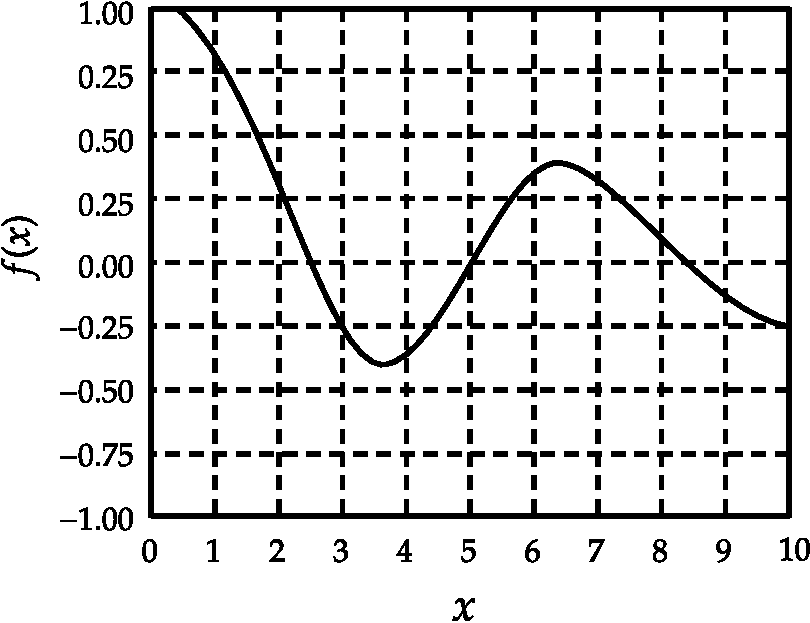
\includegraphics[height=6cm,width=8cm]{diagram-20211005(12)-crop}
	\end{figure}
	\begin{tasks}(2)
		\task[\textbf{A.}]  The Bessel function $J_{0}(x)$
		\task[\textbf{B.}] $\cos x$
		\task[\textbf{C.}] $e^{-x} \cos x$
		\task[\textbf{D.}] $\frac{1}{x} \cos x$
	\end{tasks}
	\item Given that $\sum_{n=0}^{\infty} H_{n}(x) \frac{t^{n}}{n !}=e^{-t^{2}+2 t x}$ the value of $H_{4}(0)$ is
	{\exyear{NET/JRF(JUNE-2013)}}
	\begin{tasks}(4)
		\task[\textbf{A.}] 12
		\task[\textbf{B.}] 6
		\task[\textbf{C.}] 24
		\task[\textbf{D.}] $-6$
	\end{tasks}
	\item   Given $\sum_{n=0}^{\infty} P_{n}(x) t^{n}=\left(1-2 x t+t^{2}\right)^{-1 / 2}$, for $|t|<1$, the value of $P_{5}(-1)$ is
	{\exyear{NET/JRF(JUNE-2014)}}
	\begin{tasks}(4)
		\task[\textbf{A.}] $0.26$
		\task[\textbf{B.}] 1
		\task[\textbf{C.}] $0.5$
		\task[\textbf{D.}] $-1$
	\end{tasks}
	\item The function $f(x)=\sum_{n=0}^{\infty} \frac{(-1)^{n}}{n !(n+1) !}\left(\frac{x}{2}\right)^{2 n+1}$, satisfies the differential equation
	{\exyear{NET/JRF(DEC-2014)}}
	\begin{tasks}(2)
		\task[\textbf{A.}]  $x^{2} \frac{d^{2} f}{d x^{2}}+x \frac{d f}{d x}+\left(x^{2}+1\right) f=0$
		\task[\textbf{B.}]  $x^{2} \frac{d^{2} f}{d x^{2}}+2 x \frac{d f}{d x}+\left(x^{2}-1\right) f=0$
		\task[\textbf{C.}] $x^{2} \frac{d^{2} f}{d x^{2}}+x \frac{d f}{d x}+\left(x^{2}-1\right) f=0$
		\task[\textbf{D.}] $x^{2} \frac{d^{2} f}{d x^{2}}-x \frac{d f}{d x}+\left(x^{2}-1\right) f=0$
	\end{tasks}
	\item
	 The Hermite polynomial $H_{n}(x)$, satisfies the differential equation
	$$
	\frac{d^{2} H_{n}}{d x^{2}}-2 x \frac{d H_{n}}{d x}+2 n H_{n}(x)=0
	$$
	The corresponding generating function $G(t, x)=\sum_{n=0}^{\infty} \frac{1}{n !} H_{n}(x) t^{n}$, satisfies the equation
	{\exyear{NET/JRF(DEC-2015)}}
	\begin{tasks}(2)
		\task[\textbf{A.}] $\frac{\partial^{2} G}{\partial x^{2}}-2 x \frac{\partial G}{\partial x}+2 t \frac{\partial G}{\partial t}=0$
		\task[\textbf{B.}] $\frac{\partial^{2} G}{\partial x^{2}}-2 x \frac{\partial G}{\partial x}-2 t^{2} \frac{\partial G}{\partial t}=0$
		\task[\textbf{C.}] $\frac{\partial^{2} G}{\partial x^{2}}-2 x \frac{\partial G}{\partial x}+2 \frac{\partial G}{\partial t}=0$
		\task[\textbf{D.}]  $\frac{\partial^{2} G}{\partial x^{2}}-2 x \frac{\partial G}{\partial x}+2 \frac{\partial^{2} G}{\partial x \partial t}=0$
	\end{tasks}
	\item A stable asymptotic solution of the equation $x_{n+1}=1+\frac{3}{1+x_{n}}$ is $x=2$. If we take $x_{n}=2+\epsilon_{n}$ and $x_{n+1}=2+\epsilon_{n+1}$, where $\epsilon_{n}$ and $\epsilon_{n+1}$ are both small, the ratio $\frac{\epsilon_{n+1}}{\epsilon_{n}}$ is approximately
	{\exyear{NET/JRF(DEC-2016)}}
	\begin{tasks}(4)
		\task[\textbf{A.}] $-\frac{1}{2}$
		\task[\textbf{B.}] $-\frac{1}{4}$
		\task[\textbf{C.}]  $-\frac{1}{3}$
		\task[\textbf{D.}] $-\frac{2}{3}$
	\end{tasks}
	\item  The Green's function satisfying
	$$
	\frac{d^{2}}{d x^{2}} g\left(x, x_{0}\right)=\delta\left(x-x_{0}\right)
	$$
	with the boundary conditions $g\left(-L, x_{0}\right)=0=g\left(L, x_{0}\right)$, is
	{\exyear{NET/JRF(JUNE-2017)}}
	\begin{tasks}(1)
		\task[\textbf{A.}] $\left\{\begin{array}{ll}\frac{1}{2 L}\left(x_{0}-L\right)(x+L), & -L \leq x<x_{0} \\ \frac{1}{2 L}\left(x_{0}+L\right)(x-L), & x_{0} \leq x \leq L\end{array}\right.$
		\task[\textbf{B.}]  $\left\{\begin{array}{ll}\frac{1}{2 L}\left(x_{0}+L\right)(x+L), & -L \leq x<x_{0} \\ \frac{1}{2 L}\left(x_{0}-L\right)(x-L), & x_{0} \leq x \leq L\end{array}\right.$
		\task[\textbf{C.}] $\left\{\begin{array}{ll}\frac{1}{2 L}\left(L-x_{0}\right)(x+L), & -L \leq x<x_{0} \\ \frac{1}{2 L}\left(x_{0}+L\right)(L-x), & x_{0} \leq x \leq L\end{array}\right.$
		\task[\textbf{D.}] $\frac{1}{2 L}(x-L)(x+L), \quad-L \leq x \leq L$
	\end{tasks}
	\item  The generating function $G(t, x)$ for the Legendre polynomials $P_{n}(t)$ is
	$$
	G(t, x)=\frac{1}{\sqrt{1-2 x t+x^{2}}}=\sum_{n=0}^{\infty} x^{n} P_{n}(t), \text { for }|x|<1
	$$
	If the function $f(x)$ is defined by the integral equation $\int_{0}^{x} f\left(x^{\prime}\right) d x^{\prime}=x G(1, x)$, it can be expressed as
	{\exyear{NET/JRF(DEC-2017)}}
	\begin{tasks}(2)
		\task[\textbf{A.}] $\sum_{n, m=0}^{\infty} x^{n+m} P_{n}(1) P_{m}\left(\frac{1}{2}\right)$
		\task[\textbf{B.}] $\sum_{n, m=0}^{\infty} x^{n+m} P_{n}(1) P_{m}(1)$
		\task[\textbf{C.}] $\sum_{n, m=0}^{\infty} x^{n-m} P_{n}(1) P_{m}(1)$
		\task[\textbf{D.}] $\sum_{n, m=0}^{\infty} x^{n-m} P_{n}(0) P_{m}(1)$
	\end{tasks}
	\item In the function $P_{n}(x) e^{-x^{2}}$ of a real variable $x, P_{n}(x)$ is polynomial of degree $n$. The maximum number of extrema that this function can have is
	{\exyear{NET/JRF(JUNE-2018)}}
	\begin{tasks}(4)
		\task[\textbf{A.}] $n+2$
		\task[\textbf{B.}]  $n-1$
		\task[\textbf{C.}] $n+1$
		\task[\textbf{D.}] $n$
	\end{tasks}
	\item  The Green's function $G\left(x, x^{\prime}\right)$ for the equation $\frac{d^{2} y(x)}{d x^{2}}+y(x)=f(x)$, with the boundary values $y(0)=y\left(\frac{\pi}{2}\right)=0$, is
	{\exyear{NET/JRF(JUNE-2018)}}
	\begin{tasks}(1)
		\task[\textbf{A.}] $G\left(x, x^{\prime}\right)=\left\{\begin{array}{ll}x\left(x^{\prime}-\frac{\pi}{2}\right), & 0<x<x^{\prime}<\frac{\pi}{2} \\ \left(x-\frac{\pi}{2}\right) x^{\prime}, & 0<x^{\prime}<x<\frac{\pi}{2}\end{array}\right.$
		\task[\textbf{B.}] $G\left(x, x^{\prime}\right)=\left\{\begin{array}{ll}-\cos x^{\prime} \sin x, & 0<x<x^{\prime}<\frac{\pi}{2} \\ -\sin x^{\prime} \cos x, & 0<x^{\prime}<x<\frac{\pi}{2}\end{array}\right.$
		\task[\textbf{C.}] $G\left(x, x^{\prime}\right)=\left\{\begin{array}{ll}\cos x^{\prime} \sin x, & 0<x<x^{\prime}<\frac{\pi}{2} \\ \sin x^{\prime} \cos x, & 0<x^{\prime}<x<\frac{\pi}{2}\end{array}\right.$
		\task[\textbf{D.}] $G\left(x, x^{\prime}\right)=\left\{\begin{array}{ll}x\left(\frac{\pi}{2}-x^{\prime}\right), & 0<x<x^{\prime}<\frac{\pi}{2} \\ x^{\prime}\left(\frac{\pi}{2}-x\right), & 0<x^{\prime}<x<\frac{\pi}{2}\end{array}\right.$
	\end{tasks}
	\item The polynomial $f(x)=1+5 x+3 x^{2}$ is written as linear combination of the Legendre polynomials
	$\left(P_{0}(x)=1, P_{1}(x), P_{2}(x)=\frac{1}{2}\left(3 x^{2}-1\right)\right)$ as $f(x)=\sum_{n} c_{n} P_{n}(x)$. The value of $c_{0}$ is
	{\exyear{NET/JRF(DEC-2018)}}
	\begin{tasks}(4)
		\task[\textbf{A.}] $\frac{1}{4}$
		\task[\textbf{B.}] $\frac{1}{2}$
		\task[\textbf{C.}]  2
		\task[\textbf{D.}]  4
	\end{tasks}
	\item The Green's function $G\left(x, x^{\prime}\right)$ for the equation $\frac{d^{2} y(x)}{d x^{2}}=f(x)$, with the boundary values $y(0)=0$ and $y(1)=0$, is
	{\exyear{NET/JRF(DEC-2018)}}
	\begin{tasks}(1)
		\task[\textbf{A.}] $G\left(x, x^{\prime}\right)=\left\{\begin{array}{ll}\frac{1}{2} x\left(1-x^{\prime}\right), & 0<x<x^{\prime}<1 \\ \frac{1}{2} x^{\prime}(1-x) & 0<x^{\prime}<x<1\end{array}\right.$
		\task[\textbf{B.}] $G\left(x, x^{\prime}\right)=\left\{\begin{array}{ll}x\left(x^{\prime}-1\right), & 0<x<x^{\prime}<1 \\ x^{\prime}(1-x) & 0<x^{\prime}<x<1\end{array}\right.$
		\task[\textbf{C.}] $G\left(x, x^{\prime}\right)=\left\{\begin{array}{ll}-\frac{1}{2} x\left(1-x^{\prime}\right), & 0<x<x^{\prime}<1 \\ \frac{1}{2} x^{\prime}(1-x) & 0<x^{\prime}<x<1\end{array}\right.$
		\task[\textbf{D.}]  $G\left(x, x^{\prime}\right)=\left\{\begin{array}{ll}x\left(x^{\prime}-1\right), & 0<x<x^{\prime}<1 \\ x^{\prime}(x-1) & 0<x^{\prime}<x<1\end{array}\right.$
	\end{tasks}
	\item  The Green's function for the differential equation $\frac{d^{2} x}{d t^{2}}+x=f(t)$, satisfying the initial conditions $x(0)=\frac{d x}{d t}(0)=0$ is\\
	$$G(t, \tau)=\left\{\begin{array}{ll}0 & \text { for } \quad 0<t<\tau \\ \sin (t-\tau) & \text { for } \quad t>\tau\end{array}\right.$$\\
	The solution of the differential equation when the source $f(t)=\theta(t)$ (the Heaviside step function) is
	{\exyear{NET/JRF(JUNE-2020)}}
	\begin{tasks}(4)
		\task[\textbf{A.}] $\sin t$
		\task[\textbf{B.}] $1-\sin t$
		\task[\textbf{C.}] $1-\cos t$
		\task[\textbf{D.}] $\cos ^{2} t-1$
	\end{tasks}
\end{enumerate}
 \colorlet{ocre1}{ocre!70!}
\colorlet{ocrel}{ocre!30!}
\setlength\arrayrulewidth{1pt}
\begin{table}[H]
	\centering
	\arrayrulecolor{ocre}
	\begin{tabular}{|p{1.5cm}|p{1.5cm}||p{1.5cm}|p{1.5cm}|}
		\hline
		\multicolumn{4}{|c|}{\textbf{Answer key}}\\\hline\hline
		\rowcolor{ocrel}Q.No.&Answer&Q.No.&Answer\\\hline
		1&\textbf{D} &2&\textbf{D}\\\hline 
		3&\textbf{A} &4&\textbf{A} \\\hline
		5&\textbf{D} &6&\textbf{C} \\\hline
		7&\textbf{A}&8&\textbf{C}\\\hline
		9&\textbf{A}&10&\textbf{B}\\\hline
		11&\textbf{C} &12&\textbf{B}\\\hline
		13&\textbf{C}&14&\textbf{D}\\\hline
		15&\textbf{C}& &\\\hline
		
	\end{tabular}
\end{table}
\begin{abox}
	Problem Set -3
\end{abox}
\begin{enumerate}[label=\color{ocre}\textbf{\arabic*.}]
	\item Green function for time dependent Schrödinger wave equation is defined as $G\left(\vec{r}, t: r^{\prime}, t^{\prime}\right)$. If $H$ is Hamiltonion of system then $G\left(\vec{r}, t: r^{\prime}, t^{\prime}\right)$ will satisfied the equation
	 \begin{tasks}(1)
		\task[\textbf{a.}]$\left(i \hbar \frac{\partial}{\partial t}-H\right) G\left(\vec{r}, t ; \vec{r}^{\prime}, t^{\prime}\right)=0$
		\task[\textbf{b.}]$\left(i \hbar \frac{\partial}{\partial t}-H\right) G\left(\vec{r}, t ; \vec{r}^{\prime}, t^{\prime}\right)=\delta\left(\vec{r}-\vec{r}^{\prime}\right)$
		\task[\textbf{c.}] $\left(i \hbar \frac{\partial}{\partial t}-H\right) G\left(\vec{r}, t ; \vec{r}^{\prime}, t^{\prime}\right)=\delta\left(t-t^{\prime}\right)$
		\task[\textbf{d.}]  $\left(i \hbar \frac{\partial}{\partial t}-H\right) G\left(\vec{r}, t ; \vec{r}^{\prime}, t^{\prime}\right)=\delta\left(\vec{r}-\vec{r}^{\prime}\right) \delta\left(t-t^{\prime}\right)$
	\end{tasks}
\begin{answer}
So the correct answer is \textbf{Option (d)}
\end{answer}
	\item $G\left(x, x_{0}\right)$ is the Green's function associated with the boundary value problem consisting of ordinary differential equation.
	$$
	\frac{d}{d x}\left(p(x) \frac{d u}{d x}\right)=f(x) \text { with } u(0)=0, u(L)=0
	$$
	The discontinuity condition on the derivative $\frac{d G\left(x, x_{0}\right)}{d x}$ at $x=x_{0}$ is
	 \begin{tasks}(4)
		\task[\textbf{a.}]0
		\task[\textbf{b.}]$p\left(x_{0}\right)$
		\task[\textbf{c.}]1
		\task[\textbf{d.}] $\frac{1}{p\left(x_{0}\right)}$
	\end{tasks}
\begin{answer}
	\begin{align*}
	\left.\frac{d G}{d x}\right|_{x=x_{0}^{+}}-\left.\frac{d G}{d x}\right|_{x=x_{i 1}^{-}}=\frac{1}{p\left(x_{0}\right)}
	\end{align*}
	So the correct answer is \textbf{Option (d)}
\end{answer}
\item Consider the steady state heat equation $\frac{d^{2} u}{d x^{2}}=f(x)$ with boundary condition,
$$
u(0)=0, u(L)=0
$$
The Green's function associated with the above equation
 \begin{tasks}(2)
	\task[\textbf{a.}]Constant
	\task[\textbf{b.}] Linear function
	\task[\textbf{c.}] Parabolic function
	\task[\textbf{d.}] Hyperbolic function
\end{tasks}
\begin{answer}
	\begin{align*}
	\intertext{The Green's function satisfies}
	\frac{d^{2} G\left(x, x_{0}\right)}{d x^{2}}&=\delta\left(x-x_{0}\right)\\
\text{	with }G\left(0, x_{0}\right)&=0\text{ and }G\left(L, x_{0}\right)=0
\intertext{Corresponding homogeneous equation is:}
\frac{d^{2} G}{d x^{2}}&=0\\
\text{Solution for }x \neq x_{0}&\text{ are, }G\left(x, x_{0}\right)= \begin{cases}a+b x_{2} & x<x_{1+} \\ c+d x, & x>x_{0}\end{cases}
	\end{align*}
		So the correct answer is \textbf{Option (b)}
\end{answer}
\item Consider the steady state heat equation $\frac{d^{2} u}{d x^{2}}=f(x)$ with boundary condition. $u(0)=0, u(L)=0$
The Green's function associated with the above equation is
 \begin{tasks}(1)
	\task[\textbf{a.}] $G\left(x, x_{0}\right)= \begin{cases}\frac{x}{L}\left(x_{0}-L\right), & 0 \leq x \leq x_{0} \\ \frac{x_{0}}{L}(x-L), & x_{0} \leq x \leq L\end{cases}$
	\task[\textbf{b.}] $G\left(x, x_{0}\right)= \begin{cases}\frac{x}{L}\left(L-x_{0}\right), & 0 \leq x \leq x_{0} \\ \frac{x_{0}}{L}(L-x), & x_{0} \leq x \leq L\end{cases}$
	\task[\textbf{c.}] $G\left(x, x_{0}\right)= \begin{cases}\sqrt{\frac{x}{L},} &\quad 0 \leq x \leq x_{0} \\ \sqrt{\frac{(x-L)}{L}}, & \quad x_{0} \leq x \leq L\end{cases}$
	\task[\textbf{d.}] $G\left(x, x_{0}\right)= \begin{cases}\sqrt{\frac{L-x}{L},}, & 0 \leq x \leq x_{0} \\ \sqrt{\frac{(x)}{L}}, & x_{0} \leq x \leq L\end{cases}$
\end{tasks}
\begin{answer}
	\begin{align*}
	\intertext{The Green's function satisfies}
	\frac{d^{2} G\left(x, x_{0}\right)}{d x^{2}}&=\delta\left(x-x_{0}\right)\\
	\text{with }G\left(0, x_{0}\right)&=0\text{ and }G\left(L, x_{0}\right)=0
	\intertext{Corresponding homogeneous equation is:}
	\frac{d^{2} G}{d x^{2}}&=0\\
	\text{Solution for }&x \neq x_{0}\text{ are}\\
	G\left(x, x_{0}\right)&= \begin{cases}a+b x, & x<x_{0} \\ c+d x, & x>x_{0}\end{cases}
	\intertext{From boundary conditions:}
	G\left(0, x_{0}\right)&=0 \Rightarrow a=0\\
	G\left(L, x_{0}\right)&=0 \Rightarrow c=-d L\\
	\therefore G\left(x, x_{0}\right)&= \begin{cases}b x, & x<x_{0} \\ d(x-L), & x>x_{0}\end{cases}\\
	\text{From continuity of }&\text{Green's function at }x=x_{0},\text{ we have}\\
	b x_{0}&=d\left(x_{0}-L\right)\\
	b&=\frac{d\left(x_{0}-L\right)}{x_{0}}\\
	\text{From discontinuity of }&\frac{\partial G}{\partial x}\text{ at }x=x_{0}\text{, we have}\\
	\left.\frac{\partial G}{\partial x}\right|&_{x=x_{0}^{+}}-\left.\frac{\partial G}{\partial x}\right|_{x=x_{0}^{-}}=1\\
	d-b&=1\\
	\Rightarrow d&=b+1 \Rightarrow d=\frac{d\left(x_{0}-L\right)}{x_{0}}+1 \Rightarrow d x_{0}=d x_{0}-d L+x_{0}\\
	\Rightarrow d&=\frac{x_{0}}{L}, b=d-1=\left(\frac{x_{0}}{L}-1\right)\\
	\therefore G\left(x, x_{0}\right)&= \begin{cases}\frac{x}{L}\left(x_{0}-L\right), & 0 \leq x \leq x_{0} \\ \frac{x_{0}}{L}(x-L), & x_{0} \leq x \leq L\end{cases}
	\end{align*}
		So the correct answer is \textbf{Option (a)}
\end{answer}
\item The differential equation defined as $\frac{d^{2} y}{d x^{2}}=f(x)$ With boundary conditions $\quad y(0)=0$ and $y^{\prime}(1)=0$
The green function $G\left(x, x_{0}\right)$ satisfy the
 \begin{tasks}(2)
	\task[\textbf{a.}]$G\left(x, x_{0}\right)= \begin{cases}x & \text { if } x<x_{0} \\ x_{0} & \text { if } x>x_{0}\end{cases}$
	\task[\textbf{b.}]$G\left(x, x_{0}\right)= \begin{cases}-x & \text { if } x<x_{0} \\ -x_{0} & \text { if } x>x_{0}\end{cases}$
	\task[\textbf{c.}]$G\left(x, x_{0}\right)= \begin{cases}x^{2} & \text { if } x<x_{0} \\ -x_{0} & \text { if } x>x_{0}\end{cases}$
	\task[\textbf{d.}] $G\left(x, x_{0}\right)= \begin{cases}-x^{2} & \text { if } x<x_{0} \\ -x_{0} & \text { if } x>x_{0}\end{cases}$
\end{tasks}
\begin{answer}
	\begin{align}
	\intertext{The corresponding non-homogenous differential equation for Green's function is}\notag\\
	\frac{\partial^{2}}{\partial x^{2}} G\left(x, x_{0}\right)&=\delta\left(x-x_{0}\right)\\
	\text{With }G\left(0, x_{0}\right)&=0\text{ and }G^{\prime}\left(1, x_{0}\right)=0\notag\notag\\
\text{	Let }&\frac{\partial^{2}}{\partial x^{2}} G\left(x, x_{0}\right)=0\notag\\
\Rightarrow G\left(x, x_{0}\right)&= \begin{cases}A x+B, & x<x_{0} \\ C x+D, & x>x_{0}\end{cases}\label{SF-01}
\intertext{Using booundary condition, we have}\notag\\
B&=0\text{ and }C=0\notag\\
\therefore&\text{ equation (\ref{SF-01}) becomes}\notag\\
G\left(x, x_{b}\right)&= \begin{cases}A x, & x<x_{0} \\ D, & x>x_{i 1}\end{cases}\notag\\
\text{From continuity of }&\left(f\left(x, x_{0}\right)\right.\text{ at }x=x_{0}\text{, we have}\notag\\
A x_{0}&=D
\intertext{From discontinuity of first derivative of Green's function i.c. $\frac{\partial G}{\partial x}$ at $x=x_{0}$ we have}
\left.\frac{\partial G}{\partial x}\right|_{x=x_{0}^{+}}-\left.\frac{\partial G}{\partial x}\right|&_{x=x_{0}^{-}}=1\notag\\
\Rightarrow 0-A&=1 \Rightarrow A=-1\notag\\
\text{and }D&=-x_{0}\notag\\
\therefore G\left(x, x_{0}\right)&= \begin{cases}-x & \text { if } x<x_{0} \notag\\ -x_{0} & \text { if } x>x_{0}\end{cases}
	\end{align}
	So the correct answer is \textbf{Option (b)}
\end{answer}
\item For real $n$ the cylindrical Bessel function of order $n$ is $J_{n}(x)$ then $J_{1 / 2}$ will converge to
 \begin{tasks}(4)
	\task[\textbf{a.}]0
	\task[\textbf{b.}]1
	\task[\textbf{c.}] $-1$
	\task[\textbf{d.}] $\frac{1}{2}$
\end{tasks}
\begin{answer}
	\begin{align*}
	{{\color{red}{Not completed}}}\\
	\end{align*}
	So the correct answer is \textbf{Option (a)}
\end{answer}
\item For real $n$ the cylindrical Bessel function is $J_{n}(x)$ of order $n$ then behavior $J_{1 / 2}$ will behave $x \approx 0$ as
 \begin{tasks}(4)
	\task[\textbf{a.}] 0
	\task[\textbf{b.}]$\sqrt{\frac{2 x}{\pi}}$
	\task[\textbf{c.}]$\sqrt{\frac{x}{\pi}}$
	\task[\textbf{d.}]  $\sqrt{\frac{x}{2 \pi}}$
\end{tasks}
\begin{answer}
	\begin{align*}
	{{\color{red}{Not completed}}}\\
	J_{n}(x)&=\sum_{0}^{\infty} \frac{(-1)^{r}}{[r \mid n+r}\left(\frac{x}{2}\right)^{n+2 r} \Rightarrow J_{1 / 2}(x)=\sum_{0}^{\infty} \frac{(-1)^{r}}{\left\lfloor\frac{1}{2}+r\right.}\left(\frac{x}{2}\right)^{\frac{1}{2}+2 r}\\
	\text{Put }r&=0 \frac{\sqrt{x / 2}}{\frac{1}{2}}=\sqrt{\frac{2 x}{\pi}} \text{where }\frac{1}{2}=\frac{\sqrt{\pi}}{2}
	\end{align*}
		So the correct answer is \textbf{Option (b)}
\end{answer}
\item For real $n$ the cylindrical Bessel function is $J_{n}(x)$ of order $n$ then behavior $J_{1 / 2}$ will equivalent to (it is given that $\underline{r} \cdot\left\lfloor r-\frac{1}{2}=\left[(2 r) 2^{-r} \sqrt{\pi}\right)\right.$
 \begin{tasks}(4)
	\task[\textbf{a.}] $\sqrt{\frac{2}{\pi}} \frac{\sin x}{\sqrt{x}}$
	\task[\textbf{b.}]$\sqrt{\frac{2}{\pi}} \frac{\sin x}{x}$
	\task[\textbf{c.}]$\sqrt{\frac{2}{\pi}} \frac{\cos x}{\sqrt{x}}$
	\task[\textbf{d.}] $\sqrt{\frac{2}{\pi}} \frac{\cos }{x}$
\end{tasks} 
\begin{answer}
	\begin{align*}
	{{\color{red}{Not completed}}}\\
	\end{align*}
\end{answer}
\item For real $n$ the cylindrical Bessel function is $J_{n}(x)$ of order $n$ then $J_{n}(x)$ will satisfied differential equation
 \begin{tasks}(1)
	\task[\textbf{a.}]$\frac{d^{2} J_{n}}{d x^{2}}+\frac{1}{x}\left(\frac{d J_{n}}{d x}\right)+\left(1+\frac{n^{2}}{x^{2}}\right) J_{n}=0$
	\task[\textbf{b.}] $\frac{d^{2} J_{n}}{d x^{2}}+\frac{1}{x}\left(\frac{d J_{n}}{d x}\right)+\left(1-\frac{n^{2}}{x^{2}}\right) J_{n}=0$
	\task[\textbf{c.}] $\frac{d^{2} J_{n}}{d x^{2}}+x\left(\frac{d J_{n}}{d x}\right)+\left(1+\frac{n^{2}}{x^{2}}\right) J_{n}=0$
	\task[\textbf{d.}] $\frac{d^{2} J_{n}}{d x^{2}}+x\left(\frac{d J_{n}}{d x}\right)+\left(1-\frac{n^{2}}{x^{2}}\right) J_{n}=0$
\end{tasks}
\begin{answer}
	\begin{align*}
\text{The Bessel function is given by }\frac{d^{2} J_{n}}{d x^{2}}+\frac{1}{x}\left(\frac{d J_{n}}{d x}\right)+\left(1-\frac{n^{2}}{x^{2}}\right) J_{n}=0
	\end{align*}
		So the correct answer is \textbf{Option (b)}
\end{answer}
\item For real $n$ the cylindrical Bessel function is $J_{n}(x)$ of order $n$ then value of $\frac{d J_{0}}{d x}$ is equivalent to 
 \begin{tasks}(4)
	\task[\textbf{a.}] $J_{1}$
	\task[\textbf{b.}]$-J_{1}$
	\task[\textbf{c.}]$2 J_{1}$
	\task[\textbf{d.}]$-2 J_{1}$
\end{tasks}
\begin{answer}
	\begin{align*}
J_{n+1}(x)=-J_{n}^{\prime}(x)+\frac{n}{x} J_{n}\text{. for }n=0, J_{1}=-J_{0}^{\prime}
	\end{align*}
		So the correct answer is \textbf{Option (b)}
\end{answer}
\item  The differential equation $x^{2} \frac{d^{2} y}{d x^{2}}+2 x \frac{d y}{d x}+\left[x^{2}-\lambda\right] y(x)=0$ is spherical Bessel's differential equation of order $n$ then value of $\lambda$ is given by
 \begin{tasks}(4)
	\task[\textbf{a.}]$n$
	\task[\textbf{b.}]$n(n+1)$
	\task[\textbf{c.}] $n(n-1)$
	\task[\textbf{d.}]  $n^{2}$
\end{tasks}
\begin{answer}
	\begin{align*}
\text{Spherical Bessel's differential equation }x^{2} \frac{d^{2} y}{d x^{2}}+2 x \frac{d y}{d x}+\left[x^{2}-n(n+1)\right] y(x)=0
	\end{align*}
		So the correct answer is \textbf{Option (b)}
\end{answer}
\item If $J_{n}(x)$ is spherical Bessel function of order $n$ if $N_{n}(x)$ is spherical Neumann function of order $n$ and $h_{n}^{\prime}$ is spherical Hankel function of type one of order $n$. Then $h_{0}^{1}$ is given by
 \begin{tasks}(4)
	\task[\textbf{a.}]$i \frac{e^{-i x}}{x}$
	\task[\textbf{b.}]$-i \frac{e^{-i x}}{x}$
	\task[\textbf{c.}] $i \frac{e^{i x}}{x}$
	\task[\textbf{d.}] $-i \frac{e^{i x}}{x}$
\end{tasks}
\begin{answer}
	\begin{align*}
		h_{n}^{1}&=J_{n}+i N_{n}\\
	J_{0}(x)&=\frac{\sin x}{x}, N_{0}(x)=-\frac{\cos x}{x} \Rightarrow h_{0}^{\prime^{\prime}}=J_{0}+i N_{0}=\frac{\sin x-i \cos x}{\because x}=-i \frac{e^{i x}}{x}
	\end{align*}
	So the correct answer is \textbf{Option (d)}
\end{answer}
\item If $J_{n}(x)$ is spherical Bessel function of order $n$ if $N_{n}(x)$ is spherical Neumann function of order $n$ and $h_{n}^{2}$ is spherical Hankel function of type two of order $n$. Then $h_{0}^{2}$ is given by
 \begin{tasks}(4)
	\task[\textbf{a.}] $i \frac{e^{-i x}}{x}$
	\task[\textbf{b.}] $-i \frac{e^{-i x}}{x}$
	\task[\textbf{c.}]$i \frac{e^{i x}}{x}$
	\task[\textbf{d.}] $-i \frac{e^{i x}}{x}$
\end{tasks}
\begin{answer}
	\begin{align*}
	h_{n}^{2}&=J_{n}-i N_{n}\\
	J_{0}(x)&=\frac{\sin x}{x},N_{0}(x)=-\frac{\cos x}{x} \Rightarrow h_{0}^{1}=J_{0}+i N_{0} \Rightarrow \frac{\sin x+i \cos x}{x}=i \frac{e^{-i x}}{x}
	\end{align*}
		So the correct answer is \textbf{Option (a)}
\end{answer}
\item If $J_{n}(x)$ is spherical Bessel function of order $n$ then $j_{0}^{\prime}(x)$ is equivalent to
 \begin{tasks}(4)
	\task[\textbf{a.}]$j_{1}(x)$
	\task[\textbf{b.}]$-j_{1}(x)$
	\task[\textbf{c.}]$\frac{j_{1}(x)}{2}$
	\task[\textbf{d.}]$-\frac{j_{1}(x)}{2}$
\end{tasks}
\begin{answer}
	\begin{align*}
	\frac{d}{d x}\left(j_{0}(x)\right)&=\frac{d}{d x}\left(\frac{\sin x}{x}\right)=\frac{\cos x}{x}-\frac{\sin x}{x^{2}}=-J_{1}(x)\\
	\text{Where }j_{1}(x)&=-\frac{\cos x}{x}+\frac{\sin x}{x^{2}}
	\end{align*}
	So the correct answer is \textbf{Option (b)}
\end{answer}
\item The solution of the differential equation $x^{2} \frac{d^{2} y}{d x^{2}}+2 x \frac{d y}{d x}+x^{2} y(x)=0$ subjected to the condition is given by $y(0)=1$.
 \begin{tasks}(4)
	\task[\textbf{a.}] $\frac{\sin x}{x}$
	\task[\textbf{b.}] $\frac{\cos x}{x}$
	\task[\textbf{c.}]$\frac{\exp (-i x)}{x}$
	\task[\textbf{d.}] $\frac{\exp i x}{x}$
\end{tasks}
\begin{answer}
	\begin{align*}
 \text{Spherical Bessel's differential equation }&x^{2} \frac{d^{2} y}{d x^{2}}+2 x \frac{d y}{d x}+\left[x^{2}-n(n+1)\right] y(x)=0\\
 \text{ then }x^{2} \frac{d^{2} y}{d x^{2}}+2 x \frac{d y}{d x}+x^{2} y(x)=0 &\text{ is spherical Bessel's differential equation for order}\\
 n&=0\\
	\text{then solution is }J_{0}(x)&=\frac{\sin x}{x}\text{ with boundary condition }y(0)=1.
	\end{align*}
	So the correct answer is \textbf{Option (a)}
\end{answer}
\item $H_{n}(x)$ is Hermite polynomials of order $n$ then $H_{n}(x)=(-1)^{n} f(x) \frac{d^{n}(W(x))}{d x^{n}}$, then $f(x)$ and $W(x)$ are respectively
 \begin{tasks}(1)
	\task[\textbf{a.}]$f(x)=\exp \left(x^{2}\right), W(x)=\exp \left(-x^{2}\right)$
	\task[\textbf{b.}]$f(x)=\exp \left(-x^{2}\right), W=\exp \left(x^{2}\right)$
	\task[\textbf{c.}] $f(x)=W(x)=\exp \left(x^{2}\right)$
	\task[\textbf{d.}] $f(x)=W(x)=\exp \left(-x^{2}\right)$
\end{tasks}
\begin{answer}
	\begin{align*}
	H_{n}(x)&=(-1)^{n} \exp \left(x^{2}\right) \frac{d^{n}\left(\exp \left(-x^{2}\right)\right)}{d x^{n}}\\
	\text{So after comparing }H_{n}(x)&=(-1)^{n} f(x) \frac{d^{n}(W(x))}{d x^{n}}\\
	f(x)&=\exp \left(x^{2}\right), W(x)=\exp \left(-x^{2}\right)
	\end{align*}
		So the correct answer is \textbf{Option (a)}
\end{answer}
\item The solution of differential equation $\frac{d^{2} y}{d x^{2}}-2 x \frac{d y}{d x}+\lambda y(x)=0$ is Hermilte polynomial of order $n$ then value of $\lambda$ is
 \begin{tasks}(4)
	\task[\textbf{a.}]$n$
	\task[\textbf{b.}] $-n$
	\task[\textbf{c.}]$2 n$
	\task[\textbf{d.}] $-2 n$
\end{tasks}
\begin{answer}
	\begin{align*}
	\frac{d^{2} y}{d x^{2}}-2 x \frac{d y}{d x}+2 n y(x)=0\text{ is Hermite differential equation}
	\end{align*}
		So the correct answer is \textbf{Option (c)}
\end{answer}
\item The Rodrigues formula for Laguerre polunomial is given by
 \begin{tasks}(2)
	\task[\textbf{a.}]$L_n(x)=\frac{e^{-x}}{n !}\left(\frac{d}{d x}\right)^{n}\left(x^{n} e^{-x}\right)$
	\task[\textbf{b.}]$L_{n}(x)=\frac{e^{x}}{n !}\left(\frac{d}{d x}\right)^{n}\left(x^{n} e^{x}\right)$
	\task[\textbf{c.}]$L_n(x)=\frac{e^{-x}}{n !}\left(\frac{d}{d x}\right)^{n}\left(x^{n} e^{x}\right)$
	\task[\textbf{d.}] $L_{n}(x)=\frac{e^{x}}{n !}\left(\frac{d}{d x}\right)^{n}\left(x^{n} e^{-x}\right)$
\end{tasks}
\begin{answer}
	\begin{align*}
	L_{n}(x)=\frac{e^{x}}{n !}\left(\frac{d}{d x}\right)^{n}\left(x^{n} e^{-x}\right)
	\end{align*}
		So the correct answer is \textbf{Option (d)}
\end{answer}
\item It is given that operator $x-\frac{d}{d x}=-\exp \left(\frac{x^{2}}{2}\right) \frac{d}{d x} \exp \left(-\frac{x^{2}}{2}\right)$
If then the normalized wave function for harmonic oscillation is $\psi(x)=\left(\pi^{1 / 2} 2^{n}\lfloor n)^{-1 / 2} \exp \left(-\frac{x^{2}}{2}\right) H_{n}(x)\right.$, then $\psi_n(x)$ is equivalent to 
 \begin{tasks}(1)
	\task[\textbf{a.}]$\psi_{n}(x)=\left(\pi^{1 / 2} 2^{n}\lfloor n)^{-1 / 2}\left(x-\frac{d}{d x}\right)^{n} \exp \left(-\frac{x^{2}}{2}\right)\right.$
	\task[\textbf{b.}] $\psi_{n}(x)=\left(\pi^{1 / 2} 2^{n}\lfloor n)^{-1 / 2}\left(x-\frac{d}{d x}\right)^{2 n} \exp \left(\frac{x^{2}}{2}\right)\right.$
	\task[\textbf{c.}] $\psi_{n}(x)=\left(\pi^{1 / 2} 2^{n}\lfloor n)^{-1 / 2}\left(x-\frac{d}{d x}\right)^{n} \exp \left(-x^{2}\right)\right.$
	\task[\textbf{d.}] $\psi_{n}(x)=\left(\pi^{k / 2} 2^{n}\lfloor n)^{-1 / 2}\left(x-\frac{d}{d x}\right)^{2 n} \operatorname{cxp}\left(-x^{2}\right)\right.$
\end{tasks}
\begin{answer}
	\begin{align*}
	H_{n}(x)&=(-1)^{n} \exp \left(x^{2}\right) \frac{d^{n}\left(\exp \left(-x^{2}\right)\right)}{d x^{n}}\\
	x-\frac{d}{d x} &=-\exp \left(\frac{x^{2}}{2}\right) \frac{d}{d x} \exp \left(-\frac{x^{2}}{2}\right) \Rightarrow\left(x-\frac{d}{d x}\right) \exp \left(-\frac{x^{2}}{2}\right) \\ &\left.=-\exp \left(\frac{x^{2}}{2}\right) \frac{d}{d x} \exp \left(-\frac{x^{2}}{2}\right)\right) \exp \left(-\frac{x^{2}}{2}\right)\\
	x \exp \left(-\frac{x^{2}}{2}\right)-\frac{d \exp \left(-\frac{x^{2}}{2}\right)}{d x}&=-\exp \left(\frac{x^{2}}{2}\right) \frac{d}{d x} \exp \left(-x^{2}\right)\\
	\Rightarrow\left(x-\frac{d}{d x}\right) \exp \left(-\frac{x^{2}}{2}\right)&=\exp \left(\frac{x^{2}}{2}\right)\left(-2 x \exp \left(-x^{2}\right)\right)=2 x \exp -\frac{x^{2}}{2}=H_{1}\left(\exp -\frac{x^{2}}{2}\right)\\
	\text{where }2 x&=H_{1}(x)\\
	\text{Similarly }\left(x-\frac{d}{d x}\right)^{n} \exp \left(-\frac{x^{2}}{2}\right)&=H_{n} \exp \left(-\frac{x^{2}}{2}\right)\\
	\psi_{n}(x)&=\left(\pi^{1 / 2} 2^{n}\lfloor n)^{-1 / 2}\left(x-\frac{d}{d x}\right)^{n} \exp \left(-\frac{x^{2}}{-2}\right)\right.
	\end{align*}
	So the correct answer is \textbf{Option (a)}
\end{answer}
\item The solution of differential equation $x \frac{d^{2} y}{d x^{2}}+(1-x) \frac{d y}{d x}+\lambda y(x)=0$ is Laguerre polynomials of order $n$ then value of $\lambda$ is
 \begin{tasks}(4)
	\task[\textbf{a.}]$n$
	\task[\textbf{b.}]$-n$
	\task[\textbf{c.}] $2 n$
	\task[\textbf{d.}] $-2 n$
\end{tasks}
\begin{answer}
	\begin{align*}
	x \frac{d^{2} y}{d x^{2}}+(1-x) \frac{d y}{d x}+n y(x)=0\text{ is Laguerre differential equation.}
	\end{align*}
	So the correct answer is \textbf{Option (a)}
\end{answer}
\item The generating function $F(x, t)=\sum_{n=0}^{\infty} P_{n}(x) t^{n}$ for the Legendre polynomials $P_{n}(x)$ is $F(x, t)=\left(1-2 x t+t^{2}\right)^{-1 / 2}$. The value of $P_{2}(-1)$ is
 \begin{tasks}(4)
	\task[\textbf{a.}]$5 / 2$
	\task[\textbf{b.}]$3 / 2$
	\task[\textbf{c.}] $+1$
	\task[\textbf{d.}] $-1$
\end{tasks}
\begin{answer}
	\begin{align*}
	\text{The generating function for Legendre polynomial is }F(x, t)&=\left(1-2 x t+t^{2}\right)^{-1 / 2}.\text{ Thus}\\P_{2}(x)=\frac{1}{2}\left(3 x^{2}-1\right) \Rightarrow P_{2}(-1)=\frac{1}{2}(3-1)=1
	\end{align*}
		So the correct answer is \textbf{Option (c)}
\end{answer}
\item If we observe plot of Bessel functions $J_{0}(x), J_{1}(x)$, and $J_{2}(x)$ we find their maxima at $x_{0}, x_{1}$ and $x_{2}$ respectively. Then which of the following is true
 \begin{tasks}(2)
	\task[\textbf{a.}]$x_{0}<x_{1}<x_{2}$
	\task[\textbf{b.}]$x_{0}>x_{1}>x_{2}$
	\task[\textbf{c.}]$x_{0}<x_{1}=x_{2}$
	\task[\textbf{d.}] $x_{0}=x_{1}<x_{2}$
\end{tasks}
\begin{answer}
	So the correct answer is \textbf{Option (a)}
\end{answer}
\item Which one of the following is correctly matched?\\
\begin{figure}[H]
	\centering
	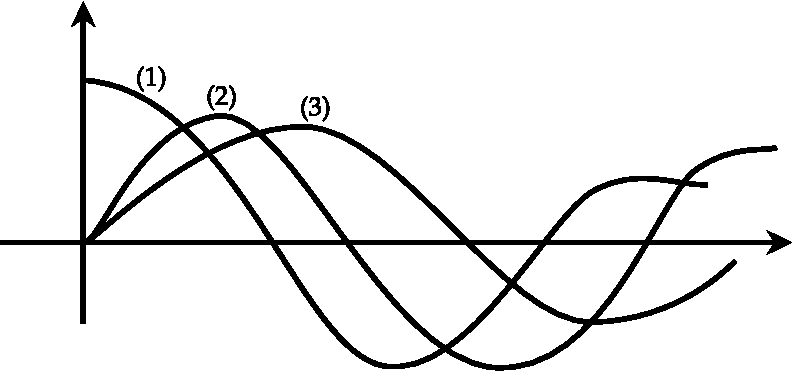
\includegraphics[height=3.5cm,width=6.5cm]{SF-01}
\end{figure}
 \begin{tasks}(2)
	\task[\textbf{a.}](1) $J_{0}$,
	(2) $J_{2}$, (3) $J_{1}$
	\task[\textbf{b.}]$(1) J_{0}$,
	(2) $J_{1}, \quad(3) J_{2}$
	\task[\textbf{c.}](1) $J_{2}$,
	(2) $J_{1}$,
	(3) $J_{0}$
	\task[\textbf{d.}] None of the above
\end{tasks}
\begin{answer}
	So the correct answer is \textbf{Option (b)}
\end{answer}
\item If the generating function of Legendre polynomial is $\frac{1}{\sqrt{1-6 t+t^{2}}}$, then coefficient of $t^{2}$ is
 \begin{tasks}(4)
	\task[\textbf{a.}] 11
	\task[\textbf{b.}]$-11$
	\task[\textbf{c.}]13
	\task[\textbf{d.}] $-13$
\end{tasks}
\begin{answer}
	\begin{align*}
	\intertext{The generating function for the polynomial solutions of the Legendre ODE is given by}
	g(x, t)&=\frac{1}{\sqrt{1-2 x t+t^{2}}}=\sum_{n=0}^{\infty} P_{n}(x) t^{n}\\
	\text{Thus }x&=3\text{ and }n=2.\\
	P_{2}(x)&=\frac{1}{2}\left(3 x^{2}-1\right) \Rightarrow P_{2}(3)=\frac{1}{2}\left(3 \times 3^{2}-1\right)=13
	\end{align*}
		So the correct answer is \textbf{Option (c)}
\end{answer}
\item Which of the following relation is true for Bessel's differential equation?
 \begin{tasks}(2)
	\task[\textbf{a.}]$J_{0}^{\prime}(x)=J_{1}(x)$
	\task[\textbf{b.}]$J_{0}^{\prime}(x)=-J_{2}(x)$
	\task[\textbf{c.}]$J_{0}^{\prime}(x)=J_{2}(x)$
	\task[\textbf{d.}] $J_{0}^{\prime}(x)=-J_{1}(x)$
\end{tasks}
\begin{answer}
	So the correct answer is \textbf{Option (d)}
\end{answer}
\item Given that $\sum_{n=0}^{\infty} H_{n}(x) \frac{t^{n}}{n !}=e^{-t^{2}+2 x x}$ the value of $H_{6}(0)$ is
 \begin{tasks}(4)
	\task[\textbf{a.}]$-120$
	\task[\textbf{b.}]$+120$
	\task[\textbf{c.}]12
	\task[\textbf{d.}]  $-12$
\end{tasks}
\begin{answer}
	\begin{align*}
	\sum_{n=0}^{\infty} I_{n}(x) \frac{t^{\prime \prime}}{n !}&=e^{-t^{2}+2 t x} \Rightarrow \sum_{n=0}^{\infty} H_{n}(0) \frac{t^{n}}{n !}=e^{-t^{2}}=1-t^{2}+\frac{t^{4}}{2 !}-\frac{t^{6}}{3 !}\\
	\Rightarrow \frac{H_{6}(0)}{6 !} t^{6}&=-\frac{1}{3 !} t^{6} \Rightarrow H_{6}(0)=-\frac{6 !}{3 !}=-120
	\end{align*}
	So the correct answer is \textbf{Option (a)}
\end{answer}
\item Given that $\sum_{n=0}^{\infty} H_{n}(x) \frac{t^{n}}{n !}=e^{-t^{2}+2 e x}$ the value of $H_{4}(0)$ is
 \begin{tasks}(4)
	\task[\textbf{a.}]12
	\task[\textbf{b.}] 6
	\task[\textbf{c.}]24
	\task[\textbf{d.}] $-6$
\end{tasks}
\begin{answer}
	\begin{align*}
	\sum_{n=0}^{\infty} H_{n}(x) \frac{t^{n}}{n !}&=e^{-t^{2}+2 t x} \Rightarrow \sum_{n=0}^{\infty} H_{n}(0) \frac{t^{n}}{n !}=e^{-t^{2}}=1-t^{2}+\frac{t^{4}}{2 !}-\frac{t^{6}}{3 !}\\
	\Rightarrow \frac{H_{4}(0)}{4 !} t^{4}&=\frac{t^{4}}{2 !} \Rightarrow H_{4}(0)=\frac{4 !}{2 !}=12
	\end{align*}
	So the correct answer is \textbf{Option (a)}
\end{answer}
\item If Hermite polynomial of order 2 is given by $H_{2}(x)=a x^{2}-2 ; a>0$, then the value of $a$ is
 \begin{tasks}(4)
	\task[\textbf{a.}]3
	\task[\textbf{b.}]4
	\task[\textbf{c.}]5
	\task[\textbf{d.}] 6
\end{tasks}
\begin{answer}
	\begin{align*}
	\intertext{Orthonormality condition,}
	\int_{-\infty}^{+\infty}\left[H_{n}(x)\right]^{2} e^{-x^{2}} d x&=2^{\prime \prime} n ! \sqrt{\pi}\\
	\text{For, }n&=2, \int_{-\infty}^{+\infty}\left(a x^{2}-2\right)^{2} e^{-x^{2}} d x=8 \sqrt{\pi}\\
\text{	Now}
	\int_{-\infty}^{+\infty}\left[H_{2}(x)\right]^{2} e^{-x^{2}} d x&=\int_{-\infty}^{+\infty}\left(a x^{2}-2\right)^{2} e^{-x^{2}} d x=\left\{a^{2} \times \frac{3}{4}+4-2 a\right\} \sqrt{\pi}
	\intertext{Thus, we have}
	\frac{3 a^{2}}{4}+4-2 a&=8 \Rightarrow 3 a^{2}-8 a-16=0 \Rightarrow 3 a^{2}-12 a+4 a-16=0\\
	\Rightarrow 3 a(a-4)+4(a-4)&=0 \Rightarrow(3 a+4)(a-4)=0\\
	\text{Thus, }a&=4
	\end{align*}
		So the correct answer is \textbf{Option (b)}
\end{answer}
\item The value of Legendre polynomial $p_{n}(x)$ for odd $n$ and $x=0$. i.e., $p_{n}(0)$ is
 \begin{tasks}(4)
	\task[\textbf{a.}]1
	\task[\textbf{b.}]0
	\task[\textbf{c.}]$-1$
	\task[\textbf{d.}]  $0.5$
\end{tasks}
\begin{answer}
	\begin{align*}
	\intertext{The generating function for Legendre polynomial is}
	\left(1-2 x t+t^{2}\right)^{-1 / 2}&=\sum_{n=0}^{\infty} p_{n}(x) t^{n}\\
	\text{Put, $x=0$, we get, }&\left(1+t^{2}\right)^{-1 / 2}=\sum p_{n}(\theta) t^{n}
	\end{align*}
		So the correct answer is \textbf{Option (b)}
\end{answer}
\item For the Legendre's polynomial $P_{n}(x)$, given below are two statements. Study these carefully and pick out the correct option.\\
Statement I: $\quad \int_{-1}^{1} x\left[P_{n}(x)\right]^{2} d x=0$\\
Statement I: $\lim _{n \rightarrow \infty}\left[\int_{-1}^{1} x P_{n}(x) P_{n+1}(x) d x\right]=0$
 \begin{tasks}(1)
	\task[\textbf{a.}]Only statement (I) is correct
	\task[\textbf{b.}]Only statement (II) is correct
	\task[\textbf{c.}]Both (I) and (II) are correct
	\task[\textbf{d.}]Neither (I) nor (II) is correet
\end{tasks}
\begin{answer}
	\begin{align*}
	\intertext{From recurrence relation we have}
	(n+1) P_{n+1}(x)&=(2 n+1) x p_{n}(x)-n p_{n-1}(x)\\
	x p_{n}(x)&=\frac{1}{(2 n+1)}\left\{(n+1) p_{n+1}(x)+n p_{n-1}(x)\right\}\\
	x\left[p_{n}(x)\right]^{2}&=\frac{1}{(2 n+1)}\left\{(n+1) p_{n}(x) p_{n+1}(x)+n p_{n}(x) p_{n-1}(x)\right\}\\
	\therefore \int_{-1}^{+1} x\left[p_{n}(x)\right]^{2} d x&=0\left\{\because \int_{-1}^{+1} p_{m}(x) p_{n}(x)=0\right.\text{ if }\left.m \neq n\right\}\\
	\therefore &\int_{-1}^{+1} x\left[p_{n}(x)\right]^{2} d x=0
	\intertext{From recurrence relation, we have}
	(n+1) p_{n+1}(x)&=(2 n+1) x p_{n}(x)-n p_{n-1}(x)\\
	(2 n+1) x p_{n}(x)&=(n+1) p_{n+1}(x)+n p_{n-1}(x)\\
	\int_{-1}^{+1}(2 n+1) x p_{n}(x) p_{n+1}(x) d x&=\int_{-1}^{+1}\left[(n+1)\left\{p_{n+1}(x)\right\}^{2}+n p_{n-1}(x) p_{n+1}(x)\right] d x\\
	=\int_{-1}^{+1}(n+1)\left\{p_{n+1}(x)\right\}^{2} d x+n \int_{-1}^{+1}& p_{n-1}(x) p_{n+1}(x) d x=(n+1) \frac{2}{2(n+1)+1}+0=\frac{2 n+2}{2 n+3}\\
	\therefore \int_{-1}^{+1} x p_{n}(x) p_{n+1}(x) d x&=\frac{2 n+2}{(2 n+1)(2 n+3)}\\
	\lim _{n \rightarrow \infty} \frac{n\left(2+\frac{2}{n}\right)}{n^{2}\left(2+\frac{1}{n}\right)\left(2+\frac{3}{n}\right)}&=\lim _{n \rightarrow \infty} \frac{\left(2+\frac{2}{n}\right)}{n\left(2+\frac{1}{n}\right)\left(2+\frac{3}{n}\right)}=0
	\end{align*}
		So the correct answer is \textbf{Option (c)}
\end{answer}
\item Which of the following statements is Incorrect about the Hermite polynomials $H_{n}(x)$ ?
 \begin{tasks}(1)
	\task[\textbf{a.}] The value of integral $\frac{1}{\sqrt{\pi}} \int_{-\infty}^{\infty} e^{-x^{2}}\left[H_{4}(x)\right]^{2} d x$ is 384
	\task[\textbf{b.}] Hermite polynomial of order $3, H_{3}(x)$, satisfies the differential equation $y^{\prime \prime}-2 x y^{\prime}+6 y=0$
	\task[\textbf{c.}] The value of $\mathrm{H}_{4}(\mathrm{l})$ is $-20$
	\task[\textbf{d.}] $H_{n}(x)=\frac{H_{n+1}(x)+2 n H_{n-1}(x)}{x}$
\end{tasks}
\begin{answer}
	\begin{align*}
	\intertext{When integrated with respect to weight function $e^{-x^{2}}$, the Hermite polynomials satisfy}
	\int_{-\infty}^{\infty} e^{-x^{2}} H_{n}(x) H_{m}(x) d x&= \begin{cases}0, & n \neq m \\ \sqrt{\pi} 2^{n} n !, & n=m\end{cases}
	\intertext{In our case $n=m=4$, hence}
	\frac{1}{\sqrt{\pi}} \int_{-\infty}^{\infty} e^{-x^{2}}\left[H_{4}(x)\right]^{2} d x&=\frac{\sqrt{\pi} 2^{4}(4 !)}{\sqrt{\pi}}=384
	\intertext{Hermite polynomial of order $n$, satisfies the differential equation}
	y^{\prime \prime}-2 x y^{\prime}+2 n y=0\\
\text{	when }n=3, y^{\prime \prime}-2 x y^{\prime}+6 y=0\\
	\text{We have }H_{4}(x)&=16 x^{4}-48 x^{2}+12\\
	\text{Therefore, }H_{4}(1)&=-48+28=-20
	\intertext{The recursion relation for Hermite polynomials is}
	H_{n+1}(x)&=2 x H_{n}(x)-2 n H_{n-1}(x) \Rightarrow H_{n}(x)=\frac{H_{n+1}(x)+2 n H_{n-1}(x)}{2 x}
	\end{align*}
		So the correct answer is \textbf{Option (d)}
\end{answer}
\item If $P_{n}(x)$ denotes the Legendre polynomials of order $n$, then which of the following statements is incorrect?
 \begin{tasks}(1)
	\task[\textbf{a.}]$P_{n}(x)=\frac{1}{2^{n} n !} \frac{d^{n}}{d x^{n}}\left[\left(x^{2}-1\right)^{n}\right]$ where $n=0,1,2 \ldots$
	\task[\textbf{b.}]The Legendre polynomials satisfy the differential equation\\$
	\left(1-x^{2}\right) \frac{d^{2} y}{d x^{2}}-2 x \frac{d y}{d x}+n(n+1) y=0
	$
	\task[\textbf{c.}] For each value of $n$ the Legendre polynomials satisfy the relation $P_{n}(1)=1$.
	\task[\textbf{d.}] The value of integral $\int_{-1}^{1}\left[P_{4}(x)\right]^{2} d x$ is $\frac{2}{7}$.
\end{tasks}
\begin{answer}
	\begin{align*}
	\intertext{Option (a) is the correct definition of Legendre polynomial. Legendre polynoimials satisfy the differential equation given in option (b). For each value of $n$ Legendre polynomials satisfy $P_{n}(1)=1$.}
	\text{Since, }\int_{-1}^{1}\left[P_{n}(x)\right]^{2} d x&=\frac{2}{2 n+1}\\
	\text{Hence, }\int_{-1}^{1}\left[P_{4}(x)\right]^{2} d x&=\frac{2}{2 \cdot 4+1}=\frac{2}{9}\\
	\text{Hence option }&(d)\text{ is incorrect.}
	\end{align*}
		So the correct answer is \textbf{Option (d)}
\end{answer}
\end{enumerate}
%\chapter{Assignment-Numerical Techniques Solutions}
\begin{enumerate}
	\item $\left. \right. $
	\begin{answer}
		Taylor's series for $y(x)$ is given by
		\begin{align*}
		y(x)&=1+x y_{0}^{\prime}+\frac{x^{2}}{2} y_{0}^{\prime \prime}+\frac{x^{3}}{6} y_{0}^{\prime \prime \prime}+\frac{x^{4}}{24} y_{0}^{i v} \ldots \ldots \ldots\\
		y^{\prime \prime}(x)&=x y^{\prime}(x)+y(x) \Rightarrow y^{\prime \prime}(0)=x y^{\prime}(0)+y(0)=1\\
		y^{\prime \prime \prime}(x)&=x y^{\prime \prime}(x)+2 y^{\prime}(x) \Rightarrow y^{\prime \prime \prime}(0)=x y^{\prime \prime}(x)+2 y^{\prime}(0)=0\\
		y^{i v}(x)&=x y^{\prime \prime \prime}+3 y^{\prime \prime} \Rightarrow y^{i v}(0)=x y^{\prime \prime \prime}(0)+3 y^{\prime \prime}(0)=3\\
		y(x)&=1+\frac{x^{2}}{2}+\frac{x^{4}}{24}(3) \ldots \ldots \ldots\\
		\Rightarrow y(0.1)&=1.0050 \Rightarrow y(0.05)=0.5025
		\end{align*}
		So the correct answer is \textbf{Option (d)}		
	\end{answer}
	\item $\left. \right. $
	\begin{answer}
		$h=0.5$; The value of $x$ and $y$ are tabulated below:
		\begin{align*}
		\begin{tabular}{|l|l|}
		\hline$x$ & $y$ \\
		\hline $0.0$ & $1.0000$ \\
		\hline $0.5$ & $0.6667$ \\
		\hline $1.0$ & $0.5000$ \\
		\hline
		\end{tabular}\\
		\text{Simpson's }&1 / 3\text{ rule}\\
		I=\int_{x_{0}}^{x_{n}} y d x&=\frac{h}{3}\left[y_{0}+4\left(y_{1}+y_{3}+\ldots .+y_{n-1}\right)+2\left(y_{2}+y_{4}+\ldots .+y_{n-2}\right)+y_{n}\right]\\
		\Rightarrow I&=\frac{0.5}{3}[1.0000+4(0.6667)+0.5]=0.6945
		\end{align*}
			So the correct answer is \textbf{Option (a)}
	\end{answer}
		\item $\left. \right. $
	\begin{answer}$\left. \right. $\\
		\begin{minipage}{0.45\textwidth}
		\begin{align*}
		I&=\frac{2}{3}\left[y_{0}+4\left(y_{1}+y_{3}\right)+2 y_{2}+y_{4}\right]\\
		&=\frac{2}{3}\left[\frac{1}{5}+4\left(\frac{1}{9}+\frac{1}{31}\right)+2 \times \frac{1}{21}+\frac{1}{69}\right]\\
		&=\frac{2}{3}\left[\frac{1}{5}+0.5734+0.09523+0.0145\right]\\
		&=\frac{2}{3}[0.2+0.5734+0.09523+0.0145]\\
		&=\frac{2}{3} \times 0.8831=0.5887
		\end{align*}
	\end{minipage}
	\begin{minipage}{0.45\textwidth}
		\begin{align*}
		\begin{tabular}{c|c}
		$x$ & $y=\frac{1}{x^{2}+5}$ \\
		\hline 0 & $\frac{1}{5}$ \\
		2 & $\frac{1}{9}$ \\
		4 & $\frac{1}{21}$ \\
		6 & $\frac{1}{31}$ \\
		8 & $\frac{1}{69}$
		\end{tabular}
		\end{align*}
	\end{minipage}
	\\So the correct answer is \textbf{Option (a)}
	\end{answer}
	\item $\left. \right. $
	\begin{answer}
		\begin{align*}
		 y(0.01)&=1+0.1(-1)=0.99\\
		y(0.02)&=0.99+0.01(-0.99)=0.9801
		\end{align*}
		So the correct answer is \textbf{Option (c)}
	\end{answer}
	\item  $\left. \right. $
\begin{answer}
	\begin{align*}
	y(0.01)&=1+0.1(-1)=0.99\\
	y(0.02)&=0.99+0.01(-0.99)=0.9801\\
	y(0.03)&=0.9801+0.01(-0.9801)=0.9703\\
	y(0.04)&=0.9703+0.01(-0.9703)=0.9606\\
	\text{The exact solution is }y&=e^{-x}\text{ and from this the value at }x=0.04\text{ is } 0.9606
	\end{align*}
		So the correct answer is \textbf{Option (d)}
\end{answer}
	\item  $\left. \right. $
	\begin{answer}
		\begin{align*}
	\text{	First, let }t_{0}&=0, y_{0}=1,\text{ and }h=1.\text{ Thus, we have}\\
	K_{0}&=f(0,1)=1, \quad K_{1}=f(0.5,1.5)=0.25, \quad K_{2}=\mathrm{f}(0.5,1.125)=0.4375 \\
	K_{3}&=\mathrm{f}(1,1.4375)=-0.4375 \\
	&\left(K_{0}+2 K_{1}+2 K_{2}+K_{3}\right) / 6=0.3229\\
	&\text{Therefore, approximation is }y_{1}=y_{0}+h 0.3229=1.322.
		\end{align*}
			So the correct answer is \textbf{Option (c)}
	\end{answer}
		\item  $\left. \right. $
	\begin{answer}
		For this data, we have the Forward difference table\\
		\begin{tabular}{|c|c|c|c|c|c|c|}
		\hline$x_{i}$ & $y_{i}$ & $\Delta y_{i}$ & $\Delta^{2} y_{3}$ & $\Delta^{3} y_{i}$ & $\Delta^{4} y_{i}$ & $\Delta^{5} y_{i}$ \\
		\hline 0 & $1.121$ & $0.002$ & $0.0005$ & $-0.0015$ & $0.002$ & $-.0025$ \\
		\hline $0.001$ & $1.123$ & $0.0025$ & $-0.0010$ & $0.0005$ & $-0.0005$ & \\
		\hline $0.002$ & $1.1255$ & $0.0015$ & $-0.0005$ & $0.0$ & & \\
		\hline $0.003$ & $1.127$ & $0.001$ & $-0.0005$ & & & \\
		\hline $0.004$ & $1.128$ & $0.0005$ & & & & \\
		\hline $0.005$ & $1.1285$ & & & & & \\
		\hline
		\end{tabular}
		\begin{align*}
	\text{	Thus, for }x&=x_{0}+h u,\text{ where }x_{0}=0, h=0.001\text{ and }u \frac{x-x_{0}}{h}\text{ we get}\\
		P_{5}(x)=& 1.121+u \times 0.002+\frac{u(u-1)}{2}(0.0005)+\frac{u(u-1)(u-2)}{3 !} \times(-0.0015) \\
		&+\frac{u(u-1)(u-2)(u-3)}{4 !}(0.002)+\frac{u(u-1)(u-2)(u-3)(u-4)}{5 !} \times(-0.0025) .
		\intertext{Thus}
		P_{5}(0.0045)&=P_{5}(0+0.001+4.5)\\
		&=1.121+0.002 \times 4.5+\frac{0.0005}{2}+4.5 \times 3.5-\frac{0.0015}{6} \times 4.5 \times 3.5 \times 2.5\\
		&+\frac{0.002}{24} \times 4.5 \times 3.5 \times 2.5 \times 1.5-\frac{0.0025}{120} \times 4.5 \times 3.5 \times 2.5 \times 1.5 \times 0.5\\
		&=1.12840045
		\end{align*}
			So the correct answer is \textbf{Option (b)}
	\end{answer}
		\item  $\left. \right. $
	\begin{answer}
		Taylor's series for $y(x)$ is given by
		\begin{align*}
		y(x)&=1+x y_{0}^{\prime}+\frac{x^{2}}{2} y_{0}^{\prime \prime}+\frac{x^{3}}{6} y_{0}^{\prime \prime \prime}+\frac{x^{4}}{24} y_{0}^{i v} \ldots \ldots \ldots\\
		y^{\prime \prime}(x)&=x y^{\prime}(x)+y(x) \Rightarrow y^{\prime \prime}(0)=x y^{\prime}(0)+y(0)=1\\
		y^{\prime \prime \prime}(x)&=x y^{\prime \prime}(x)+2 y^{\prime}(x) \Rightarrow y^{\prime \prime \prime}(0)=x y^{\prime \prime}(x)+2 y^{\prime}(0)=0\\
		y^{i v}(x)&=x y^{\prime \prime \prime}+3 y^{\prime \prime} \Rightarrow y^{i v}(0)=x y^{\prime \prime \prime}(0)+3 y^{\prime \prime}(0)=3\\
		y(x)&=1+\frac{x^{2}}{2}+\frac{x^{4}}{24}(3) \ldots \ldots \ldots\\
		\Rightarrow y(0.1)&=1.0050
		\end{align*}
			So the correct answer is \textbf{Option (a)}
	\end{answer}
	\item  $\left. \right. $
	\begin{answer}
		\begin{align*}
		\text{Taking origin at }0.65, h&=0.01\text{ and }x=0.6538\\
		\therefore p&=\frac{0 \cdot 6538-0 \cdot 65}{0 \cdot 01}=38\\
		\text{The difference table is}&\\
	\intertext{	Using Gauss's forward interpolation formula}
		\frac{p(p-1)}{2 !} \Delta^{2} y&+\frac{(p+1) p(p-1)}{3 !} \Delta^{3} y-1+\cdot \\
		10^{7} y_{0} 38=6420292+(0 \cdot 38)(73473)&+\frac{(0 \cdot 38)(0 \cdot 38-1)}{2}(-962)+\cdot \cdot=6448325 \\
		\therefore y_{0} 38&=0 \cdot 6448325
		\end{align*}
			So the correct answer is \textbf{Option (a)}
	\end{answer}



\begin{align*}
\renewcommand*{\arraystretch}{1.2}
\begin{tabular}{|p{1cm}| p{.5cm}|p{1.5cm}|p{1.2cm} |p{1.2cm}|p{1.2cm}|p{1.2cm}|p{1.2cm}|p{1.2cm}|}
\hline
x&p&$10^7\ y$&$10^7\ \Delta y$&$10^7\ \Delta^2 y$&$10^7\ \Delta^3 y$&$10^7\ \Delta^4 y$&$10^7\ \Delta^5 y$&$10^7\ \Delta^6 y$\\
\hline
 & & &76349& & & & &\\
 \hline 
 0.63&-2&6270463& &-955& & & &\\
 \hline
  & & &75394& &$-4$& & &  \\
  \hline
  0.64&-1&6345857& &-959& &1& & \\
  \hline
   & & &74435& &-3& &1& \\
   \hline
\end{tabular}
\end{align*}	

	
	
	
	
	
	
	
	
	
	
	
	
	
	
	
	
	
	
	
	
	
	
	
\end{enumerate}
%\chapter{Assignment-Matrices}
\section{MCQ}
\begin{enumerate}
	\item The eigen value of matrix $A=\left(\begin{array}{lll}1 & 0 & 1 \\ 0 & 1 & 0 \\ 1 & 0 & 1\end{array}\right)$ is
	 \begin{tasks}(2)
		\task[\textbf{a.}] $\lambda=1,0,2$
		\task[\textbf{b.}]$\lambda=-1,2,2$
		\task[\textbf{c.}] $\lambda=0,0,3$
		\task[\textbf{d.}] $\lambda=1,1,1$
	\end{tasks}
	\item The eigen value of matrix $A=\left(\begin{array}{ccc}1 & \sqrt{8} & 0 \\ \sqrt{8} & 1 & \sqrt{8} \\ 0 & \sqrt{8} & 1\end{array}\right)$ is
	 \begin{tasks}(2)
		\task[\textbf{a.}]$\lambda=1,0,2$
		\task[\textbf{b.}]$\lambda=-1,2,2$
		\task[\textbf{c.}]$\lambda=-3,1,5$
		\task[\textbf{d.}]$\lambda=1,1,1$
	\end{tasks}
	\item The eigen value of matrix $A=\left(\begin{array}{lll}0 & 1 & 0 \\ 1 & 0 & 1 \\ 0 & 1 & 0\end{array}\right)$ is
	 \begin{tasks}(2)
		\task[\textbf{a.}]$\lambda=-1,0,1$
		\task[\textbf{b.}]$\lambda=0,-2,2$
		\task[\textbf{c.}]$\lambda=0,0,0$
		\task[\textbf{d.}]  $\lambda=-\sqrt{2}, 0, \sqrt{2}$
	\end{tasks}
	\item The eigen value of matrix $A=\left(\begin{array}{lll}0 & 1 & 1 \\ 1 & 0 & 1 \\ 1 & 1 & 0\end{array}\right)$ is
	 \begin{tasks}(2)
		\task[\textbf{a.}] $\lambda=-1,-1,2$
		\task[\textbf{b.}]$\lambda=0,-2,2$
		\task[\textbf{c.}] $\lambda=0,0,0$
		\task[\textbf{d.}] $\lambda=-\sqrt{2}, 0, \sqrt{2}$
	\end{tasks}
	\item The degenerate eigen value of matrix $A=\left(\begin{array}{lll}1 & 1 & 1 \\ 1 & 1 & 1 \\ 1 & 1 & 1\end{array}\right)$ is
	 \begin{tasks}(2)
		\task[\textbf{a.}]0
		\task[\textbf{b.}]1
		\task[\textbf{c.}]2
		\task[\textbf{d.}] 3
	\end{tasks}
	\item The eigen vector of matrix $A=\left(\begin{array}{lll}1 & 0 & 1 \\ 0 & 1 & 0 \\ 1 & 0 & 1\end{array}\right)$ corresponding to eigen value 0 is
	 \begin{tasks}(2)
		\task[\textbf{a.}] $\left[\begin{array}{l}1 \\ 0 \\ 0\end{array}\right]$
		\task[\textbf{b.}]$\left[\begin{array}{c}1 \\ 0 \\ -1\end{array}\right]$
		\task[\textbf{c.}] $\left[\begin{array}{l}1 \\ 0 \\ 1\end{array}\right]$
		\task[\textbf{d.}]  $\left[\begin{array}{c}1 \\ -1 \\ 0\end{array}\right]$
	\end{tasks}
	\item The eigen vector of matrix $A=\left(\begin{array}{ccc}1 & \sqrt{8} & 0 \\ \sqrt{8} & 1 & \sqrt{8} \\ 0 & \sqrt{8} & 1\end{array}\right)$ corresponding to eigen value 5 is
	 \begin{tasks}(2)
		\task[\textbf{a.}]$\left[\begin{array}{c}1 \\ \sqrt{2} \\ 1\end{array}\right]$
		\task[\textbf{b.}]$\left[\begin{array}{c}1 \\ -\sqrt{2} \\ 1\end{array}\right]$
		\task[\textbf{c.}] $\left[\begin{array}{c}\sqrt{2} \\ 1 \\ 1\end{array}\right]$
		\task[\textbf{d.}]  $\left[\begin{array}{c}-\sqrt{2} \\ 1 \\ 1\end{array}\right]$
	\end{tasks}
	\item The eigen vectors of matrix $A=\left(\begin{array}{ccc}0 & 1 & 0 \\ 1 & 0 & 1 \\ 0 & 1 & 0\end{array}\right)$ corresponding to eigen values $-\sqrt{2}, 0, \sqrt{2}$ are respectively
	 \begin{tasks}(2)
		\task[\textbf{a.}] $\left[\begin{array}{c}1 \\ -\sqrt{2} \\ 1\end{array}\right],\left[\begin{array}{c}1 \\ 0 \\ -1\end{array}\right],\left[\begin{array}{c}1 \\ \sqrt{2} \\ 1\end{array}\right]$
		\task[\textbf{b.}]$\left[\begin{array}{c}1 \\ \sqrt{2} \\ 1\end{array}\right],\left[\begin{array}{c}1 \\ 0 \\ -1\end{array}\right],\left[\begin{array}{c}1 \\ -\sqrt{2} \\ 1\end{array}\right]$
		\task[\textbf{c.}]$\left[\begin{array}{c}1 \\ -\sqrt{2} \\ 1\end{array}\right],\left[\begin{array}{c}1 \\ \sqrt{2} \\ 1\end{array}\right],\left[\begin{array}{c}1 \\ 0 \\ -1\end{array}\right]$
		\task[\textbf{d.}]  $\left[\begin{array}{c}1 \\ 0 \\ -1\end{array}\right],\left[\begin{array}{c}1 \\ -\sqrt{2} \\ 1\end{array}\right],\left[\begin{array}{c}1 \\ \sqrt{2} \\ 1\end{array}\right]$
	\end{tasks}
	\item If one of the eigen vector of matrix $A=\left(\begin{array}{lll}0 & 1 & 1 \\ 1 & 0 & 1 \\ 1 & 1 & 0\end{array}\right)$ corresponding to eigen value $-1$ is $\left[\begin{array}{c}-2 \\ 1 \\ 1\end{array}\right]$ then other orthogonal eigen vector for same eigen value is
	 \begin{tasks}(2)
		\task[\textbf{a.}]$\left[\begin{array}{c}0 \\ 1 \\ -1\end{array}\right] \quad$
		\task[\textbf{b.}]$\left[\begin{array}{c}-4 \\ 2 \\ 2\end{array}\right]$
		\task[\textbf{c.}]$\left[\begin{array}{l}1 \\ 0 \\ 1\end{array}\right]$
		\task[\textbf{d.}] $\left[\begin{array}{c}1 \\ -1 \\ 0\end{array}\right]$
	\end{tasks}
	\item If one of the eigen vector of matrix $A=\left(\begin{array}{lll}1 & 1 & 1 \\ 1 & 1 & 1 \\ 1 & 1 & 1\end{array}\right)$ corresponding to eigen value 0 is $\left[\begin{array}{c}0 \\ 1 \\ -1\end{array}\right]$ then other orthogonal eigen vector for same eigen value is
	 \begin{tasks}(2)
		\task[\textbf{a.}] $\left[\begin{array}{c}-2 \\ 1 \\ 1\end{array}\right]$
		\task[\textbf{b.}]$\left[\begin{array}{c}0 \\ 2 \\ -2\end{array}\right]$
		\task[\textbf{c.}]$\left[\begin{array}{l}1 \\ 0 \\ 1\end{array}\right]$
		\task[\textbf{d.}]  $\left[\begin{array}{c}1 \\ -1 \\ 0\end{array}\right]$
	\end{tasks}
	\item A square matrix $3 \times 3$ is given by $A=\left[\begin{array}{lll}2 & 0 & 0 \\ 0 & 1 & 1 \\ 0 & 1 & 1\end{array}\right]$ is diagonalized in eigenvector of
	matrix $S=\left[\begin{array}{ccc}1 & 0 & 0 \\ 0 & \frac{1}{\sqrt{2}} & \frac{1}{\sqrt{2}} \\ 0 & -\frac{1}{\sqrt{2}} & \frac{1}{\sqrt{2}}\end{array}\right] .$ Which one of the following is matrix $A$ in the diagonal form in the
	basis of $S$ ?
	 \begin{tasks}(2)
		\task[\textbf{a.}] $\left[\begin{array}{lll}2 & 0 & 0 \\ 0 & 2 & 0 \\ 0 & 0 & 0\end{array}\right] \quad$ 
		\task[\textbf{b.}] $\left[\begin{array}{lll}0 & 0 & 0 \\ 0 & 2 & 0 \\ 0 & 0 & 2\end{array}\right] \quad$ 
		\task[\textbf{c.}]$\left[\begin{array}{lll}2 & 0 & 0 \\ 0 & 0 & 0 \\ 0 & 0 & 2\end{array}\right] \quad$
		\task[\textbf{d.}] $\left[\begin{array}{lll}1 & 0 & 2 \\ 0 & 1 & 0 \\ 0 & 0 & 2\end{array}\right]$
	\end{tasks}
	\item Consider the matrix $M=\left(\begin{array}{lll}1 & 1 & 1 \\ 1 & 1 & 1 \\ 1 & 1 & 1\end{array}\right) .$ The eigenvalues of $M$ are
	 \begin{tasks}(2)
		\task[\textbf{a.}] $0,1,2$
		\task[\textbf{b.}]$0,0,3$
		\task[\textbf{c.}]$1,1,1$
		\task[\textbf{d.}] $-1,1,3$
	\end{tasks}
	\item Consider the matrix $M=\left(\begin{array}{lll}1 & 1 & 1 \\ 1 & 1 & 1 \\ 1 & 1 & 1\end{array}\right)$. The exponential of $M$ simplifies to $(I$ is the $3 \times 3$ identity matrix)
	 \begin{tasks}(2)
		\task[\textbf{a.}]$e^{M}=I+\left(\frac{e^{3}-1}{3}\right) M$
		\task[\textbf{b.}] $e^{M}=I+M+\frac{M^{2}}{2 !}$
		\task[\textbf{c.}] $e^{M}=I+3^{3} M$
		\task[\textbf{d.}]  $e^{M}=(e-1) M$
	\end{tasks}
	\item The eigenvalues of the matrix $\left(\begin{array}{lll}2 & 3 & 0 \\ 3 & 2 & 0 \\ 0 & 0 & 1\end{array}\right)$ are
	 \begin{tasks}(2)
		\task[\textbf{a.}]$5,2,-2$
		\task[\textbf{b.}]$-5,-1,-1$
		\task[\textbf{c.}]$5,1,-1$
		\task[\textbf{d.}] $-5,1,1$
	\end{tasks}
	\item The eigen values of the matrix $A=\left(\begin{array}{ccc}1 & 2 & 3 \\ 2 & 4 & 6 \\ 3 & 6 & 9\end{array}\right)$ are
	 \begin{tasks}(2)
		\task[\textbf{a.}]$(1,4,9)$
		\task[\textbf{b.}] $(0,7,7)$
		\task[\textbf{c.}]$(0,1,13)$
		\task[\textbf{d.}] $(0,0,14)$
	\end{tasks}
	\item The eigenvalues of the antisymmetric matrix, $A=\left(\begin{array}{ccc}0 & -n_{3} & n_{2} \\ n_{3} & 0 & -n_{1} \\ -n_{2} & n_{1} & 0\end{array}\right)$ where $n_{1}, n_{2}$ and $n_{3}$ are the components of a unit vector, are
	 \begin{tasks}(2)
		\task[\textbf{a.}]$0, i,-i$
		\task[\textbf{b.}]$0,1,-1$
		\task[\textbf{c.}]$0,1+i,-1,-i$
		\task[\textbf{d.}] $0,0,0$
	\end{tasks}
	\item Consider the matrix $M=\left(\begin{array}{ccc}0 & 2 i & 3 i \\ -2 i & 0 & 6 i \\ -3 i & -6 i & 0\end{array}\right)$. The eigenvalues of $M$ are
	 \begin{tasks}(2)
		\task[\textbf{a.}]$-5,-2,7$
		\task[\textbf{b.}]$-7,0,7$
		\task[\textbf{c.}]$-4 i, 2 i, 2 i$
		\task[\textbf{d.}] $2,3,6$
	\end{tasks}
	\item The column vector $\left(\begin{array}{l}a \\ b \\ a\end{array}\right)$ is a simultaneous eigenvector of
	$A=\left(\begin{array}{lll}0 & 0 & 1 \\ 0 & 1 & 0 \\ 1 & 0 & 0\end{array}\right)$ and $B=\left(\begin{array}{lll}0 & 1 & 1 \\ 1 & 0 & 1 \\ 1 & 1 & 0\end{array}\right)$, if
	 \begin{tasks}(2)
		\task[\textbf{a.}] $b=0$ or $a=0$
		\task[\textbf{b.}] $b=a$ or $b=-2 a$
		\task[\textbf{c.}] $b=2 a$ or $b=-a$
		\task[\textbf{d.}]  $b=a / 2$ or $b=-a / 2$
	\end{tasks}
\item Let $\alpha$ and $\beta$ be complex numbers. Which of the following sets of matrices forms a group under matrix multiplication?
	 \begin{tasks}(2)
		\task[\textbf{a.}] $\left(\begin{array}{ll}\alpha & \beta \\ 0 & 0\end{array}\right)$
		\task[\textbf{b.}] $\left(\begin{array}{lr}1 & \alpha \\ \beta & 1\end{array}\right)$, where $\alpha \beta \neq 1$
		\task[\textbf{c.}] $\left(\begin{array}{cc}\alpha & \alpha^{*} \\ \beta & \beta^{*}\end{array}\right)$, where $\alpha \beta^{*}$ is real
		\task[\textbf{d.}]  $\left(\begin{array}{cc}\alpha & \beta \\ -\beta^{*} & \alpha^{*}\end{array}\right)$, where $|\alpha|^{2}+|\beta|^{2}=1$
	\end{tasks}
	\item A $3 \times 3$ matrix $M$ has $\operatorname{Tr}[M]=6, \operatorname{Tr}\left[M^{2}\right]=26$ and $\operatorname{Tr}\left[M^{3}\right]=90$. Which of the following can be a possible set of eigenvalues of $M$ ?
	 \begin{tasks}(2)
		\task[\textbf{a.}]$\{1,1,4\}$
		\task[\textbf{b.}]$\{-1,0,7\}$
		\task[\textbf{c.}]$\{-1,3,4\}$
		\task[\textbf{d.}] $\{2,2,2\}$
	\end{tasks}
	\item The matrix $A=\frac{1}{\sqrt{3}}\left[\begin{array}{cc}1 & 1+i \\ 1-i & -1\end{array}\right]$ is
	 \begin{tasks}(2)
		\task[\textbf{a.}]Orthogonal
		\task[\textbf{b.}] Symmetric
		\task[\textbf{c.}]anti-symmetric
		\task[\textbf{d.}] Unitary
	\end{tasks}
	\item If $H$ is Hermitian matrix then matrix $A=\exp (i H)$ is
	 \begin{tasks}(2)
		\task[\textbf{a.}] Hermitian
		\task[\textbf{b.}]Unitary
		\task[\textbf{c.}]Skew Hermitian
		\task[\textbf{d.}] Identity
	\end{tasks}
	\item The matrix $A=\left(\begin{array}{ccc}0 & 1 & 0 \\ 1 & 0 & 0 \\ 0 & 0 & 2\end{array}\right)$ is diagonalize in the basis of unitary matrices $U$ and get the diagonalise matrix $\left(\begin{array}{ccc}2 & 0 & 0 \\ 0 & 1 & 0 \\ 0 & 0 & -1\end{array}\right)$ then matrix $U$ is
	 \begin{tasks}(2)
		\task[\textbf{a.}]$\left(\begin{array}{ccc}0 & 0 & 1 \\ \frac{1}{\sqrt{2}} & \frac{1}{\sqrt{2}} & 0 \\ \frac{1}{\sqrt{2}} & -\frac{1}{\sqrt{2}} & 0\end{array}\right)$
		\task[\textbf{b.}]$\left(\begin{array}{ccc}0 & 0 & 1 \\ \frac{1}{\sqrt{2}} & \frac{1}{\sqrt{2}} & 0 \\ -\frac{1}{\sqrt{2}} & \frac{1}{\sqrt{2}} & 0\end{array}\right)$
		\task[\textbf{c.}] $\left(\begin{array}{ccc}0 & 0 & 0 \\ 0 & \frac{1}{\sqrt{2}} & \frac{1}{\sqrt{2}} \\ 1 & \frac{1}{\sqrt{2}} & -\frac{1}{\sqrt{2}}\end{array}\right)$
		\task[\textbf{d.}]  $\left(\begin{array}{ccc}0 & 1 & 0 \\ \frac{1}{\sqrt{2}} & 0 & \frac{1}{\sqrt{2}} \\ \frac{1}{\sqrt{2}} & 0 & -\frac{1}{\sqrt{2}}\end{array}\right)$
	\end{tasks}
	\item Given a $2 \times 2$ unitary matrix $U$ satisfying $U^{\dagger} U=U U^{\dagger}=1$ with $\operatorname{det} U=e^{i \varphi}$, one can construct a unitary matrix $V\left(V^{\dagger} V=V V^{\dagger}=1\right)$ with det $V=1$ from it by
	 \begin{tasks}(1)
		\task[\textbf{a.}] Multiplying $U$ by $e^{-i \varphi / 2}$
		\task[\textbf{b.}] Multiplying any single element of $U$ by $e^{-i \varphi}$
		\task[\textbf{c.}] Multiplying any row or column of $U$ by $e^{-i \varphi / 2}$
		\task[\textbf{d.}]  Multiplying $U$ by $e^{-i \varphi}$
	\end{tasks}
	\item Consider an $n \times n(n>1)$ matrix $A$, in which $A_{i j}$ is the product of the indices $i$ and $j$ (namely $A_{i j}=i j$ ). The matrix $A$
	 \begin{tasks}(1)
		\task[\textbf{a.}]Has one degenerate eigevalue with degeneracy $(n-1)$
		\task[\textbf{b.}]Has two degenerate eigenvalues with degeneracies 2 and $(n-2)$
		\task[\textbf{c.}]Has one degenerate eigenvalue with degeneracy $n$
		\task[\textbf{d.}] Does not have any degenerate eigenvalue
	\end{tasks}
	\item Two matrices $A$ and $B$ are said to be similar if $B=P^{1} A P$ for some invertible matrix $P$. Which of the following statements is NOT TRUE?
	 \begin{tasks}(2)
		\task[\textbf{a.}] $\operatorname{Det} A=\operatorname{Det} B$
		\task[\textbf{b.}] Trace of $A=$ Trace of $B$
		\task[\textbf{c.}]$A$ and $B$ have the same eigenvectors
		\task[\textbf{d.}]  $A$ and $B$ have the same eigenvalues
	\end{tasks}
	\item A $3 \times 3$ matrix has elements such that its trace is 11 and its determinant is 36 . The eigenvalues of the matrix are all known to be positive integers. The largest eigenvalues of the matrix is
	 \begin{tasks}(2)
		\task[\textbf{a.}]18
		\task[\textbf{b.}]12
		\task[\textbf{c.}]9
		\task[\textbf{d.}] 6
	\end{tasks}
	\item The inverse of matrix $M=\left(\begin{array}{lll}0 & 1 & 1 \\ 0 & 0 & 1 \\ 1 & 0 & 0\end{array}\right)$ is
	 \begin{tasks}(2)
		\task[\textbf{a.}]$M-1$
		\task[\textbf{b.}]$M^{2}-1$
		\task[\textbf{c.}] $I-M^{2}$
		\task[\textbf{d.}] $I-M$
	\end{tasks}
       \section{MSQ}  
 \item For matrix $A=\left(\begin{array}{lll}5 & 0 & 2 \\ 0 & 1 & 0 \\ 2 & 0 & 2\end{array}\right)$, which of the following statements are true?
                 \begin{tasks}(1)
                	\task[\textbf{a.}]The degenerate eigen value is 1
                	\task[\textbf{b.}]One of the eigen vector corresponding to degenerate eigen value is $\left[\begin{array}{c}1 \\ 0 \\ -2\end{array}\right]$
                	\task[\textbf{c.}]The eigen vector corresponding to nondegenerate eigen value is $\left[\begin{array}{l}2 \\ 0 \\ 1\end{array}\right]$
                	\task[\textbf{d.}] The eigen vector corresponding to nondegenerate eigen value is $\left[\begin{array}{l}0 \\ 2 \\ 1\end{array}\right]$   
                \end{tasks}
 \item   For matrix $A=\left(\begin{array}{lll}1 & 1 & 0 \\ 1 & 1 & 0 \\ 0 & 0 & 0\end{array}\right)$, which of the following statements are true?    
                 \begin{tasks}(1)
                	\task[\textbf{a.}]The degenerate eigen value is 0
                	\task[\textbf{b.}]One of the eigen vector corresponding to degenerate eigen value is $\left[\begin{array}{c}1 \\ -1 \\ 0\end{array}\right]$
                	\task[\textbf{c.}]One of the eigen vector corresponding to degenerate eigen value is $\left[\begin{array}{l}0 \\ 0 \\ 1\end{array}\right]$
                	\task[\textbf{d.}] The eigen vector corresponding to nondegenerate eigen value is $\left[\begin{array}{l}1 \\ 1 \\ 0\end{array}\right]$
                \end{tasks}
  \item For matrix $A=\left(\begin{array}{ccc}5 & 0 & \sqrt{3} \\ 0 & 3 & 0 \\ \sqrt{3} & 0 & 3\end{array}\right)$, which of the following statements are true?
  \begin{tasks}(1)
 	\task[\textbf{a.}]The eigen value are $2,3,6$
 	\task[\textbf{b.}]The eigen value are 2, 4, 5
 	\task[\textbf{c.}]Eigen vector corresponding eigen value2 is $\left[\begin{array}{c}1 \\ 0 \\ \sqrt{3}\end{array}\right]$
 	\task[\textbf{d.}] Eigen vector corresponding eigen value 2 is $\left[\begin{array}{c}\sqrt{3} \\ 0 \\ 1\end{array}\right]$
 \end{tasks}               
 \item  Which one of following is correct 
   \begin{tasks}(1)
  	\task[\textbf{a.}] If $A^{\dagger}=A$ and $B^{\dagger}=-B$ Then $A B+B A$ is skew Hermitian
  	\task[\textbf{b.}] If $A^{\dagger}=A$ and $B^{\dagger}=-B$ Then $A B+B A$ is Hermitian
  	\task[\textbf{c.}]If $A^{\dagger}=A$ and $B^{\dagger}=-B \quad i(A B+B A)$ is skew Hermitian
  	\task[\textbf{d.}] $A^{\dagger}=A$ and $B^{\dagger}=-B i(A B+B A)$ is Hermitian    
  \end{tasks}              
\item  Which of the following is correct for matrix $A=\left(\begin{array}{lll}1 & 0 & 0 \\ 0 & 0 & 1 \\ 0 & 1 & 0\end{array}\right)$             
   \begin{tasks}(2)
  	\task[\textbf{a.}] It is its own inverse
  	\task[\textbf{b.}]It is its own transpose
  	\task[\textbf{c.}] It has eigen value $\pm 1$
  	\task[\textbf{d.}]  It is orthogonal matrix.
  \end{tasks}              
\section{NAT}              
  \item The degenerate eigenvalue of the matrix $\left[\begin{array}{ccc}4 & -1 & -1 \\ -1 & 4 & -1 \\ -1 & -1 & 4\end{array}\right]$ is (your answer should be an integer)-------------      
\item  The minimum eigenvalues of the matrix $\left(\begin{array}{lll}0 & 1 & 0 \\ 1 & 0 & 1 \\ 0 & 1 & 0\end{array}\right)$ is...........               
  \item The degenerate eigen value of matrix $A=\left[\begin{array}{lll}0 & 0 & 1 \\ 0 & 1 & 0 \\ 1 & 0 & 0\end{array}\right]$ is given by
\item  The inverse of matrix $A=\left[\begin{array}{lll}0 & 0 & 1 \\ 0 & 1 & 0 \\ 1 & 0 & 0\end{array}\right]$ is   
 \begin{tasks}(2)
	\task[\textbf{a.}]$\left[\begin{array}{ccc}0 & 0 & -1 \\ 0 & -1 & 0 \\ -1 & 0 & 0\end{array}\right]$
	\task[\textbf{b.}]$\left[\begin{array}{ccc}0 & 0 & -1 \\ 0 & -1 & 0 \\ 1 & 0 & 0\end{array}\right]$
	\task[\textbf{c.}]$\left[\begin{array}{ccc}0 & 0 & -1 \\ 0 & 1 & 0 \\ 1 & 0 & 0\end{array}\right]$
	\task[\textbf{d.}] $\left[\begin{array}{lll}0 & 0 & 1 \\ 0 & 1 & 0 \\ 1 & 0 & 0\end{array}\right]$
\end{tasks}                
 \item  The eigenvalue of matrix $A=\left(\begin{array}{lll}1 & 0 & 1 \\ 0 & 1 & 0 \\ 1 & 0 & 1\end{array}\right)$ is         
  \begin{tasks}(2)
 	\task[\textbf{a.}]$\lambda=1,0,2$
 	\task[\textbf{b.}]$\lambda=-1,2,2$
 	\task[\textbf{c.}]$\lambda=0,0,3$
 	\task[\textbf{d.}]$\lambda=1,1,1$ 
 \end{tasks}
 \item The eigenvalue of matrix $A=\left(\begin{array}{ccc}1 & \sqrt{8} & 0 \\ \sqrt{8} & 1 & \sqrt{8} \\ 0 & \sqrt{8} & 1\end{array}\right)$ is
  \begin{tasks}(2)
 	\task[\textbf{a.}]$\lambda=1,0,2$
 	\task[\textbf{b.}]$\lambda=-1,2,2$
 	\task[\textbf{c.}]$\lambda=-3,1,5$
 	\task[\textbf{d.}] $\lambda=1,1,1$
 \end{tasks}
 \item The eigenvalue of matrix $A=\left(\begin{array}{lll}0 & 1 & 0 \\ 1 & 0 & 1 \\ 0 & 1 & 0\end{array}\right)$ is
  \begin{tasks}(2)
 	\task[\textbf{a.}] $\lambda=-1,0,1$
 	\task[\textbf{b.}] $\lambda=0,-2,2$
 	\task[\textbf{c.}]$\lambda=0,0,0$
 	\task[\textbf{d.}]  $\lambda=-\sqrt{2}, 0, \sqrt{2}$
 \end{tasks}
\item The eigenvalue of matrix $A=\left(\begin{array}{lll}0 & 1 & 1 \\ 1 & 0 & 1 \\ 1 & 1 & 0\end{array}\right)$ is
  \begin{tasks}(2)
 	\task[\textbf{a.}]$\lambda=-1,-1,2$
 	\task[\textbf{b.}]$\lambda=0,-2, \quad 2$
 	\task[\textbf{c.}]$\lambda=0,0,0$
 	\task[\textbf{d.}]  $\lambda=-\sqrt{2}, 0, \sqrt{2}$
 \end{tasks}
\item The eigenvector of matrix $A=\left(\begin{array}{lll}1 & 0 & 1 \\ 0 & 1 & 0 \\ 1 & 0 & 1\end{array}\right)$ corresponding to eigenvalue 0 is
  \begin{tasks}(2)
 	\task[\textbf{a.}]$\left[\begin{array}{l}1 \\ 0 \\ 0\end{array}\right]$
 	\task[\textbf{b.}]$\left[\begin{array}{c}1 \\ 0 \\ -1\end{array}\right]$
 	\task[\textbf{c.}]$-\left[\begin{array}{l}1 \\ 0 \\ 1\end{array}\right] .$
 	\task[\textbf{d.}] $\left[\begin{array}{c}1 \\ -1 \\ 0\end{array}\right]$
 \end{tasks}
 \item 69 The eigenvector of matrix $A=\left(\begin{array}{ccc}1 & \sqrt{8} & 0 \\ \sqrt{8} & 1 & \sqrt{8} \\ 0 & \sqrt{8} & 1\end{array}\right)$ corresponding to eigenvalue 5 is
  \begin{tasks}(2)
 	\task[\textbf{a.}]$\left[\begin{array}{c}1 \\ \sqrt{2} \\ 1\end{array}\right]$
 	\task[\textbf{b.}]$\left[\begin{array}{c}1 \\ -\sqrt{2} \\ 1\end{array}\right]$
 	\task[\textbf{c.}]$\left[\begin{array}{c}\sqrt{2} \\ 1 \\ 1\end{array}\right]$
 	\task[\textbf{d.}] $\left[\begin{array}{c}-\sqrt{2} \\ 1 \\ 1\end{array}\right]$
 \end{tasks}
 \item 70 The eigen vectors of matrix $A=\left(\begin{array}{lll}0 & 1 & 0 \\ 1 & 0 & 1 \\ 0 & 1 & 0\end{array}\right)$ corresponding to eigen values $-\sqrt{2}, 0, \sqrt{2}$ are respectively
  \begin{tasks}(2)
 	\task[\textbf{a.}]$\left[\begin{array}{c}1 \\ -\sqrt{2} \\ 1\end{array}\right],\left[\begin{array}{c}1 \\ 0 \\ -1\end{array}\right],\left[\begin{array}{c}1 \\ \sqrt{2} \\ 1\end{array}\right]$
 	\task[\textbf{b.}]$\left[\begin{array}{c}1 \\ \sqrt{2} \\ 1\end{array}\right],\left[\begin{array}{c}1 \\ 0 \\ -1\end{array}\right],\left[\begin{array}{c}1 \\ -\sqrt{2} \\ 1\end{array}\right]$
 	\task[\textbf{c.}] $\left[\begin{array}{c}1 \\ -\sqrt{2} \\ 1\end{array}\right],\left[\begin{array}{c}1 \\ \sqrt{2} \\ 1\end{array}\right],\left[\begin{array}{c}1 \\ 0 \\ -1\end{array}\right]$
 	\task[\textbf{d.}] $\left[\begin{array}{c}1 \\ 0 \\ -1\end{array}\right],\left[\begin{array}{c}1 \\ -\sqrt{2} \\ 1\end{array}\right],\left[\begin{array}{c}1 \\ \sqrt{2} \\ 1\end{array}\right]$
 \end{tasks}
 \item 71 If one of the eigenvector of matrix $A=\left(\begin{array}{lll}0 & 1 & 1 \\ 1 & 0 & 1 \\ 1 & 1 & 0\end{array}\right)$ corresponding to eigenvalue $-1$ is $\left[\begin{array}{c}-2 \\ 1 \\ 1\end{array}\right]$ then other orthogonal eigen vector for same eigen value is
  \begin{tasks}(2)
 	\task[\textbf{a.}]$\left[\begin{array}{c}0 \\ 1 \\ -1\end{array}\right]$
 	\task[\textbf{b.}]$\left[\begin{array}{c}-4 \\ 2 \\ 2\end{array}\right]$
 	\task[\textbf{c.}] $\left[\begin{array}{l}1 \\ 0 \\ 1\end{array}\right]$
 	\task[\textbf{d.}]  $\left[\begin{array}{c}1 \\ -1 \\ 0\end{array}\right]$
 \end{tasks}
 \item 72 If one of the eigen vector of matrix $A=\left(\begin{array}{lll}1 & 1 & 1 \\ 1 & 1 & 1 \\ 1 & 1 & 1\end{array}\right)$ corresponding to eigen value 0 is $\left[\begin{array}{c}0 \\ 1 \\ -1\end{array}\right]$ then other orthogonal eigen vector for same eigen value is
  \begin{tasks}(2)
 	\task[\textbf{a.}]$\left[\begin{array}{c}-2 \\ 1 \\ 1\end{array}\right]$
 	\task[\textbf{b.}]$\left[\begin{array}{c}0 \\ 2 \\ -2\end{array}\right]$
 	\task[\textbf{c.}]$\left[\begin{array}{l}1 \\ 0 \\ 1\end{array}\right]$
 	\task[\textbf{d.}] $\left[\begin{array}{c}1 \\ -1 \\ 0\end{array}\right]$
 \end{tasks}
 \item 73  A $3 \times 3$ matrix $M$ has $\operatorname{Tr}[M]=6, \operatorname{Tr}\left[M^{2}\right]=26$ and $\operatorname{Tr}\left[M^{3}\right]=90$. Which of the following can be a possible set of eigenvalues of $M$ ?
      \begin{tasks}(2)
     	\task[\textbf{a.}]$\{1,1,4\}$
     	\task[\textbf{b.}]$\{-1,0,7\}$
     	\task[\textbf{c.}]$\{-1,3,4\}$
     	\task[\textbf{d.}] $\{2,2,2\}$
     \end{tasks}
\item     Q74. Consider an $n \times n(n>1)$ matrix $A$, in which $A_{i j}$ is the product of the indices $i$ and $j$ (namely $\left.A_{i j}=i j\right)$. The matrix $A$
      \begin{tasks}(2)
     	\task[\textbf{a.}]has one degenerate eigevalue with degeneracy $(n-1)$
     	\task[\textbf{b.}]has two degenerate eigenvalues with degeneracies 2 and $(n-2)$
     	\task[\textbf{c.}]has one degenerate eigenvalue with degeneracy $n$
     	\task[\textbf{d.}] does not have any degenerate eigenvalue
     \end{tasks}
 \item     Q75. A $3 \times 3$ matrix has elements such that its trace is 11 and its determinant is 36 . The eigenvalues of the matrix are all known to be positive integers. The largest eigenvalues of the matrix is
     \begin{tasks}(2)
    	\task[\textbf{a.}]18
    	\task[\textbf{b.}]12
    	\task[\textbf{c.}]9
    	\task[\textbf{d.}] 6
    \end{tasks} 
\item Q76. The inverse of matrix $M=\left(\begin{array}{lll}0 & 1 & 1 \\ 0 & 0 & 1 \\ 1 & 0 & 0\end{array}\right)$ is
  \begin{tasks}(2)
    	\task[\textbf{a.}]$M-I$
    	\task[\textbf{b.}]$M^{2}-I$
    	\task[\textbf{c.}]$I-M^{2}$
    	\task[\textbf{d.}] $I-M$. 
    \end{tasks}
\item Q77. Consider the matrix $M=\left(\begin{array}{ccc}0 & 2 i & 3 i \\ -2 i & 0 & 6 i \\ -3 i & -6 i & 0\end{array}\right)$. The eigenvalues of $M$ are
 \begin{tasks}(2)
	\task[\textbf{a.}]$-5,-2,7$
	\task[\textbf{b.}]$-7,0,7$
	\task[\textbf{c.}]$-4 i, 2 i, 2 i$
	\task[\textbf{d.}] $2,3,6$ 
\end{tasks}       
 \item Q78. The matrix $A=\frac{1}{\sqrt{3}}\left[\begin{array}{cc}1 & 1+i \\ 1-i & -1\end{array}\right]$.
 is
  \begin{tasks}(2)
 	\task[\textbf{a.}]Orthogonal
 	\task[\textbf{b.}]symmetric
 	\task[\textbf{c.}] anti-symmetric
 	\task[\textbf{d.}]  Unitary    
 \end{tasks}    
\item Q79. If $H$ is Hermitian matrix then matrix $A=\exp (i H)$ is
  \begin{tasks}(2)
 	\task[\textbf{a.}] IIermitian
 	\task[\textbf{b.}] Unitary
 	\task[\textbf{c.}] Skew Hermitian
 	\task[\textbf{d.}] Identity     
 \end{tasks}    
\item Q80. Which one of following is correct?
      \begin{tasks}(2)
     	\task[\textbf{a.}] If $A^{\dagger}=A$ and $B^{\dagger}=-B$, then $A B+B A$ is skew Hermitian
     	\task[\textbf{b.}]If $A^{\dagger}=A$ and $B^{\dagger}=-B$, then $A B+B A$ is Hermitian
     	\task[\textbf{c.}] If $A^{\dagger}=A$ and $B^{\dagger}=-B$, then $-i(A B+B A)$ is skew Hermitian
     	\task[\textbf{d.}]  If $A^{\dagger}=A$ and $B^{\dagger}=-B$, then $i(A B+B A)$ is skew Hermitian
     \end{tasks}
\item Q81. A square matrix $3 \times 3$ is given by $A=\left[\begin{array}{ccc}2 & 0 & 0 \\ 0 & 1 & 1 \\ 0 & 1 & 1\end{array}\right]$ is diagonalized in eigenvector of matrix $S=\left[\begin{array}{ccc}1 & 0 & 0 \\ 0 & \frac{1}{\sqrt{2}} & \frac{1}{\sqrt{2}} \\ 0 & -\frac{1}{\sqrt{2}} & \frac{1}{\sqrt{2}}\end{array}\right]$. Which one of the following is the diagonal matrix of $A$ in form in the basis of $S$ ?
\begin{tasks}(2)
     	\task[\textbf{a.}] $\left[\begin{array}{lll}2 & 0 & 0 \\ 0 & 2 & 0 \\ 0 & 0 & 0\end{array}\right]$
     	\task[\textbf{b.}]$\left[\begin{array}{lll}0 & 0 & 0 \\ 0 & 2 & 0 \\ 0 & 0 & 2\end{array}\right]$
     	\task[\textbf{c.}] $\left[\begin{array}{lll}2 & 0 & 0 \\ 0 & 0 & 0 \\ 0 & 0 & 2\end{array}\right]$
     	\task[\textbf{d.}] $\left[\begin{array}{lll}1 & 0 & 2 \\ 0 & 1 & 0 \\ 0 & 0 & 2\end{array}\right]$
     \end{tasks}
\item    Q82. The column vector $\left(\begin{array}{l}a \\ b \\ a\end{array}\right)$ is a simultaneous eigenvector of
$A=\left(\begin{array}{lll}0 & 0 & 1 \\ 0 & 1 & 0 \\ 1 & 0 & 0\end{array}\right)$ and $B=\left(\begin{array}{lll}0 & 1 & 1 \\ 1 & 0 & 1 \\ 1 & 1 & 0\end{array}\right)$, if  
 \begin{tasks}(2)
	\task[\textbf{a.}]$b=0$ or $a=0$
	\task[\textbf{b.}]$b=a$ or $b=-2 a$
	\task[\textbf{c.}]$b=2 a$ or $b=-a$
	\task[\textbf{d.}] $b=a / 2$ or $b=-a / 2$
\end{tasks}
\item Q83. Two matrices $A$ and $B$ are said to be similar if $B=P^{-1} A P$ for some invertible matrix $P$. Which of the following statements is NOT TRUE?
   \begin{tasks}(2)
  	\task[\textbf{a.}] $\operatorname{Det} A=\operatorname{Det} B$
  	\task[\textbf{b.}] Trace of $A=$ Trace of $B$
  	\task[\textbf{c.}]$\dot{A}$ and $B$ have the same eigenvectors
  	\task[\textbf{d.}] $A$ and $B$ have the same eigenvalues
  \end{tasks}   
\item Q84. The matrix $A=\left(\begin{array}{lll}0 & 1 & 0 \\ 1 & 0 & 0 \\ 0 & 0 & 2\end{array}\right)$ is diagonalize in the basis of unitary matrices $U$ and get the diagonalise matrix $\left(\begin{array}{ccc}2 & 0 & 0 \\ 0 & 1 & 0 \\ 0 & 0 & -1\end{array}\right)$ then matrix $U$ is     
 \begin{tasks}(2)
	\task[\textbf{a.}]$\left(\begin{array}{ccc}0 & 0 & 1 \\ \frac{1}{\sqrt{2}} & \frac{1}{\sqrt{2}} & 0 \\ \frac{1}{\sqrt{2}} & -\frac{1}{\sqrt{2}} & 0\end{array}\right)$
	\task[\textbf{b.}]$\left(\begin{array}{ccc}0 & 0 & 1 \\ \frac{1}{\sqrt{2}} & \frac{1}{\sqrt{2}} & 0 \\ -\frac{1}{\sqrt{2}} & \frac{1}{\sqrt{2}} & 0\end{array}\right)$
	\task[\textbf{c.}]$\left(\begin{array}{ccc}0 & \frac{1}{\sqrt{2}} & \frac{1}{\sqrt{2}} \\ 0 & \frac{1}{\sqrt{2}} & -\frac{1}{\sqrt{2}} \\ 1 & 0 & 0\end{array}\right)$
	\task[\textbf{d.}] $\left(\begin{array}{ccc}0 & 1 & 0 \\ \frac{1}{\sqrt{2}} & 0 & \frac{1}{\sqrt{2}} \\ \frac{1}{\sqrt{2}} & 0 & -\frac{1}{\sqrt{2}}\end{array}\right)$
\end{tasks}     
     
     
     
     
     
     
     
     
\end{enumerate}

%\chapter{Assignment-Matrices-Solutions}
\begin{enumerate}
	\item  $\left. \right. $
	\begin{answer}
		\begin{align*}
		\text{For eigen value }|A-\lambda I|&=0\\
		\left|\begin{array}{ccc}
		1-\lambda & 0 & 1-\lambda \\
		0 & 1-\lambda & 0 \\
		1 & 0 & 1-\lambda
		\end{array}\right|&=(1-\lambda)\left[(1-\lambda)^{2}-0\right]+0+1[-(1-\lambda)]=0 \\
		\Rightarrow-\lambda^{3}+3 \lambda^{2}-2 \lambda&=0 \Rightarrow \lambda=0,1,2
		\end{align*}
		So the correct answer is \textbf{Option (a)}
	\end{answer}
	\item  $\left. \right. $
	\begin{answer}
		\begin{align*}
	\text{ For eigen value }|A-\lambda I|&=0\\
		\left|\begin{array}{ccc}
		1-\lambda & \sqrt{8} & 0 \\
		\sqrt{8} & (1-\lambda) & \sqrt{8} \\
		0 & \sqrt{8} & (1-\lambda)
		\end{array}\right|&=(1-\lambda)\left[(1-\lambda)^{2}-8\right]+\sqrt{8}[\sqrt{8}(1-\lambda)] \\
		-\lambda^{3}+3 \lambda^{2}-3 \lambda+1&=0 \Rightarrow \lambda=-3,1,5
		\end{align*}
			So the correct answer is \textbf{Option (c)}
	\end{answer}
	\item $\left. \right. $
	\begin{answer}
		\begin{align*}
	\text{For eigen value }|A-\lambda I|&=0\\
		\left|\begin{array}{ccc}
		-\lambda & 1 & 0 \\
		1 & -\lambda & 1 \\
		0 & 1 & -\lambda
		\end{array}\right|&=0 \Rightarrow-\lambda\left(\lambda^{2}-1\right)+1[(\lambda)]=0 \Rightarrow-\lambda^{3}+2 \lambda=0 \\
		\text { eigenvalue } \lambda&=0, \sqrt{2},-\sqrt{2}
		\end{align*}
		So the correct answer is \textbf{Option (d)}
	\end{answer}
	\item $\left. \right. $
	\begin{answer}
		\begin{align*}
		 \text{For eigen value }|A-\lambda I|&=0\\
		\left|\begin{array}{ccc}
		-\lambda & 1 & 1 \\
		1 & -\lambda & 1 \\
		1 & 1 & -\lambda
		\end{array}\right|&=0 \Rightarrow-\lambda\left[\left(\lambda^{2}-1\right)\right]+1(1+\lambda)+1(1+\lambda)=0 \\
		\Rightarrow-\lambda^{3}+3 \lambda+2&=0 \Rightarrow \lambda=-1,-1,2
		\end{align*}
		So the correct answer is \textbf{Option (a)}		
	\end{answer}
	\item $\left. \right. $
	\begin{answer}
		\begin{align*}
	\text{ For eigen value }|A-\lambda I|&=0\\
		\left|\begin{array}{ccc}
		1-\lambda & 1 & 1 \\
		1 & 1-\lambda & 1 \\
		1 & 1 & 1-\lambda
		\end{array}\right|&=0 \Rightarrow(1-\lambda)\left[\left(1-\lambda^{2}\right)-1\right]+1[1-(1-\lambda)]+1[1-(1-\lambda)]&=0 \\
		\Rightarrow-\lambda^{3}+3 \lambda^{2}=0 \Rightarrow \lambda=0,0,3
		\end{align*}
		So the correct answer is \textbf{Option (a)}	
	\end{answer}
	\item $\left. \right. $
	\begin{answer}
		\begin{align*}
		 For eigen value |A-\lambda I|&=0\\
		\left|\begin{array}{ccc}
		1-\lambda & 0 & 1-\lambda \\
		0 & 1-\lambda & 0 \\
		1 & 0 & 1-\lambda
		\end{array}\right|&=(1-\lambda)\left[(1-\lambda)^{2}-0\right]+0+1[-(1-\lambda)]=0 \\
		\Rightarrow-\lambda^{3}+3 \lambda^{2}-2 \lambda&=0 \Rightarrow \lambda=0,1,2\\
		\text{Eigen vector can be determine by }A X_{1}&=\lambda X_{1} \Rightarrow\left[\begin{array}{lll}1 & 0 & 1 \\ 0 & 1 & 0 \\ 1 & 0 & 1\end{array}\right]\left[\begin{array}{l}x_{1} \\ x_{2} \\ x_{3}\end{array}\right]=\lambda\left[\begin{array}{l}x_{1} \\ x_{2} \\ x_{3}\end{array}\right]\\
	\text{	For }\lambda=0,
		\left[\begin{array}{lll}
		1 & 0 & 1 \\
		0 & 1 & 0 \\
		1 & 0 & 1
		\end{array}\right]\left[\begin{array}{l}
		x_{1} \\
		x_{2} \\
		x_{3}
		\end{array}\right]=0\left[\begin{array}{l}
		x_{1} \\
		x_{2} \\
		x_{3}
		\end{array}\right]& \Rightarrow x_{1}+x_{3}=0, x_{2}=x_{2}, x_{1}+x_{3}=0 \Rightarrow x_{1}=-x_{3} \text { and } x_{2}=0\\
		X_{1}&=\left[\begin{array}{c}
		x_{1} \\
		0 \\
		-x_{1}
		\end{array}\right]=x_{1}\left[\begin{array}{c}
		1 \\
		0 \\
		-1
		\end{array}\right]\\
		\text{From orthogonal relation }X_{1}^{T} X_{1}&=1 \Rightarrow x_{1}=\frac{1}{\sqrt{2}} \Rightarrow X_{1}=\frac{1}{\sqrt{2}}\left[\begin{array}{c}1 \\ 0 \\ -1\end{array}\right]
		\end{align*}
		So the correct answer is \textbf{Option (b)}
	\end{answer}
	\item $\left. \right. $
	\begin{answer}
		\begin{align*}
	\text{ For eigen value }|A-\lambda I|&=0\\
		\left|\begin{array}{ccc}
		1-\lambda & \sqrt{8} & 0 \\
		\sqrt{8} & (1-\lambda) & \sqrt{8} \\
		0 & \sqrt{8} & (1-\lambda)
		\end{array}\right|&=(1-\lambda)\left[(1-\lambda)^{2}-8\right]+\sqrt{8}[\sqrt{8}(1-\lambda)] \\
		-\lambda^{3}+3 \lambda^{2}-3 \lambda+1&=0 \Rightarrow \lambda=-3,1,5\\
		\text{eigen vector can be determine by }A X_{1}&=\lambda_{1} X_{1}
	\text{	For }\lambda=5,\\
	{\left[\begin{array}{ccc}1 & \sqrt{8} & 0 \\ \sqrt{8} & 1 & \sqrt{8} \\ 0 & \sqrt{8} & 1\end{array}\right]\left[\begin{array}{l}x_{1} \\ x_{2} \\ x_{3}\end{array}\right]=5\left[\begin{array}{l}x_{1} \\ x_{2} \\ x_{3}\end{array}\right] }&\\
	x_{1}+\sqrt{8} x_{2}=5 x_{1}, \sqrt{8} x_{1}+x_{2}+\sqrt{8} x_{3}&=5 x_{2}, \sqrt{8} x_{2}+x_{3}=5 x_{3}\\
	\Rightarrow x_{1}=x_{3}, x_{2}=\sqrt{2} x_{1} \quad X_{1}=\left[\begin{array}{c}x_{1} \\ \sqrt{2} x_{1} \\ x_{1}\end{array}\right] \Rightarrow X_{1}&=x_{1}\left[\begin{array}{c}1 \\ \sqrt{2} \\ 1\end{array}\right]\\
	\text{Form orthogonality condition }x_{1}=\frac{1}{2}, X_{1}&=\frac{1}{2}\left[\begin{array}{c}1 \\ \sqrt{2} \\ 1\end{array}\right]
		\end{align*}
			So the correct answer is \textbf{Option (a)}
	\end{answer}
	\item $\left. \right. $
	\begin{answer}
		\begin{align*}
		 \text{For eigen value }|A-\lambda I|&=0\\
		\left|\begin{array}{ccc}
		-\lambda & 1 & 0 \\
		1 & -\lambda & 1 \\
		0 & 1 & -\lambda
		\end{array}\right|=0 \Rightarrow-&\lambda\left(\lambda^{2}-1\right)+1[(\lambda)]=0 \Rightarrow-\lambda^{3}+2 \lambda=0\\
	\text{	eigenvalue }\lambda=0, \sqrt{2},-\sqrt{2}\\
		\text{eigen vector can be determine by }A X_{1}&=\lambda_{1} X_{1}
	\text{	For }\lambda=-\sqrt{2}\\
		\left[\begin{array}{lll}
		0 & 1 & 0 \\
		1 & 0 & 1 \\
		0 & 1 & 0
		\end{array}\right]\left[\begin{array}{l}
		x_{1} \\
		x_{2} \\
		x_{3}
		\end{array}\right]=-\sqrt{2}\left[\begin{array}{l}
		x_{1} \\
		x_{2} \\
		x_{3}
		\end{array}\right] \Rightarrow x_{2}&=-\sqrt{2} x_{1}, x_{1}+x_{3}=-\sqrt{2} x_{2}, x_{2}=-\sqrt{2} x_{3}\\
		\Rightarrow x_{1}&=x_{3}, x_{2}=-\sqrt{2} x_{1}\\
		X_{1}=\left[\begin{array}{c}x_{1} \\ -\sqrt{2} x_{1} \\ x_{1}\end{array}\right] \text{. From orthogonality condition, }X_{1}^{T} X_{1}&=1 \Rightarrow x_{1}=\frac{1}{2} \Rightarrow X_{1}=\frac{1}{2}\left[\begin{array}{c}1 \\ -\sqrt{2} \\ 1\end{array}\right]\\
	\text{	For }\lambda&=0\\
		\left[\begin{array}{lll}
		0 & 1 & 0 \\
		1 & 0 & 1 \\
		0 & 1 & 0
		\end{array}\right]\left[\begin{array}{l}
		x_{1} \\
		x_{2} \\
		x_{3}
		\end{array}\right]=0\left[\begin{array}{c}
		x_{1} \\
		x_{2} \\
		x_{3}
		\end{array}\right] \Rightarrow x_{2}=0, x_{1}+x_{3}&=0, \Rightarrow x_{1}=-x_{3} \Rightarrow X_{2}=\left[\begin{array}{c}
		x_{1} \\
		0 \\
		-x_{1}
		\end{array}\right]\\
		\text{From orthogonality condition }X_{2}^{T} X_{2}&=1 \Rightarrow x_{1}=\frac{1}{\sqrt{2}} \Rightarrow X_{2}=\frac{1}{\sqrt{2}}\left[\begin{array}{c}1 \\ 0 \\ -1\end{array}\right]\\
		\text{For }\lambda&=\sqrt{2},\\
		\left[\begin{array}{lll}
		0 & 1 & 0 \\
		1 & 0 & 1 \\
		0 & 1 & 0
		\end{array}\right]\left[\begin{array}{l}
		x_{1} \\
		x_{2} \\
		x_{3}
		\end{array}\right]=\sqrt{2}\left[\begin{array}{l}
		x_{1} \\
		x_{2} \\
		x_{3}
		\end{array}\right] \Rightarrow x_{2}=\sqrt{2} x_{1}, x_{1}+x_{3}&=\sqrt{2} x_{2}, x_{2}=\sqrt{2} x_{3} \Rightarrow x_{1}=x_{3}\\
		\Rightarrow X_{3}=\left[\begin{array}{c}x_{1} \\ \sqrt{2} x_{1} \\ x_{1}\end{array}\right] .\text{ From orthogonality condition }X_{3}{ }^{T} X_{3}=1 \Rightarrow x_{1}&=\frac{1}{2} \Rightarrow X_{3}=\frac{1}{2}\left[\begin{array}{c}1 \\ \sqrt{2} \\ 1\end{array}\right]
		\end{align*}
		So the correct answer is \textbf{Option (a)}
	\end{answer}
	\item $\left. \right. $
	\begin{answer}
		\begin{align*}
		\text{For eigen value }|A-\lambda I|&=0
		X_{1}=\frac{1}{2}\left[\begin{array}{c}-2 \\ 1 \\ 1\end{array}\right]\\
		\left|\begin{array}{ccc}-\lambda & 1 & 1 \\ 1 & -\lambda & 1 \\ 1 & 1 & -\lambda\end{array}\right|&=0 \Rightarrow-\lambda\left[\left(\lambda^{2}-1\right)\right]+1(1+\lambda)+1(1+\lambda)=0\\
		\Rightarrow-\lambda^{3}+3 \lambda+2&=0 \Rightarrow \lambda=-1,-1,2\\
		\text{Eigen vector can be determine by }A X_{1}&=\lambda_{1} X_{1}\\
	\text{	For }\lambda&=-1\\
	\left[\begin{array}{lll}0 & 1 & 1 \\ 1 & 0 & 1 \\ 1 & 1 & 0\end{array}\right]\left[\begin{array}{l}x_{1} \\ x_{2} \\ x_{3}\end{array}\right]=-1\left[\begin{array}{c}x_{1} \\ x_{2} \\ x_{3}\end{array}\right] \Rightarrow x_{2}+x_{3}&=-x_{1}, \quad x_{1}+x_{3}=-x_{2}, x_{1}+x_{2}=-x_{3} \Rightarrow x_{1}+x_{2}+x_{3}=0\\
	\text{if }X_{1}&=\left[\begin{array}{c}-\left(x_{2}+x_{3}\right) \\ x_{2} \\ x_{3}\end{array}\right]\text{ if }\Rightarrow x_{2}=k_{1} x_{3}=k_{2}\\
	X_{1}&=\left[\begin{array}{c}
	-\left(k_{1}+k_{2}\right) \\
	k_{1} \\
	k_{2}
	\end{array}\right] \text { if } k_{1}=k_{2}\\
	X_{1}&=k_{1}\left[\begin{array}{c}-2 \\ 1 \\ 1\end{array}\right]\text{ from orthogonality condition }X_{1}^{T} X_{1}=1 \Rightarrow k_{1}=\frac{1}{2}\\
	X_{1}&=\frac{1}{2}\left[\begin{array}{c}-2 \\ 1 \\ 1\end{array}\right]\\
	\text{For }\lambda&=-1\text{ similarly if }k_{1}=1, k_{2}=-1\\
	\text{Then }X_{2}=\left[\begin{array}{c}0 \\ 1 \\ -1\end{array}\right] \quad X_{2}&=\frac{1}{\sqrt{2}}\left[\begin{array}{c}0 \\ 1 \\ -1\end{array}\right]
		\end{align*}
	So the correct answer is \textbf{Option (a)}
	\end{answer}
	\item $\left. \right. $
	\begin{answer}
		\begin{align*}
		 \text{For eigen value }|A-\lambda I|&=0\\
		\left|\begin{array}{ccc}
		1-\lambda & 1 & 1 \\
		1 & 1-\lambda & 1 \\
		1 & 1 & 1-\lambda
		\end{array}\right|&=0 \Rightarrow(1-\lambda)\left[\left(1-\lambda^{2}\right)-1\right]+1[1-(1-\lambda)]+1[1-(1-\lambda)]=0\\
		\Rightarrow-\lambda^{3}+3 \lambda^{2}&=0 \Rightarrow \lambda=0,0,3\\
	\text{	eigen vector can be determine }by A X_{1}&=\lambda_{1} X_{1}\\
		\text{For }\lambda&=0,\\
		\left[\begin{array}{lll}
		1 & 1 & 1 \\
		1 & 1 & 1 \\
		1 & 1 & 1
		\end{array}\right]\left[\begin{array}{l}
		x_{1} \\
		x_{2} \\
		x_{3}
		\end{array}\right]&=0\left[\begin{array}{l}
		x_{1} \\
		x_{2} \\
		x_{3}
		\end{array}\right] \Rightarrow x_{1}+x_{2}+x_{3}=0, x_{1}+x_{2}+x_{3}=0, x_{1}+x_{2}+x_{3}=0\\
		\text{Now }x_{1}&=-x_{2}-x_{3}\text{, if }x_{2}=-1, x_{3}=1 \Rightarrow x_{1}=0\\
		X_{1}&=\left[\begin{array}{c}
		-x_{2}-x_{3} \\
		x_{2} \\
		x_{3}
		\end{array}\right] \Rightarrow X_{1}=\left[\begin{array}{c}
		0 \\
		1 \\
		-1
		\end{array}\right]=X_{1}=\frac{1}{\sqrt{2}}\left[\begin{array}{c}
		0 \\
		1 \\
		-1
		\end{array}\right]\\
	\text{	For }\lambda&=0, X_{2}=\left[\begin{array}{c}-x_{2}-x_{3} \\ x_{2} \\ x_{3}\end{array}\right]\text{ is orthogonal to }X_{1}.\\
	\frac{1}{\sqrt{2}}\left(\begin{array}{lll}
	0 & 1 & -1
	\end{array}\right)\left[\begin{array}{c}
	-x_{2}-x_{3} \\
	x_{2} \\
	x_{3}
	\end{array}\right]&=0 \Rightarrow x_{2}=x_{3} \Rightarrow X_{2}=\left[\begin{array}{c}
	-2 x_{2} \\
	x_{2} \\
	x_{2}
	\end{array}\right]\\
	\text{From orthogonality condition, }X_{2}^{T} X_{2}&=1 \Rightarrow x_{2}=\frac{1}{\sqrt{6}} \Rightarrow X_{2}=\frac{1}{\sqrt{6}}\left[\begin{array}{c}-2 \\ 1 \\ 1\end{array}\right]
		\end{align*}
		So the correct answer is \textbf{Option (a)}
	\end{answer}
		\item $\left. \right. $
	\begin{answer}
		\begin{align}
	\text{$A$ diagonalised }&=S^{-1} A S\label{AMS-01}\\
	S&=\left[\begin{array}{ccc}1 & 0 & 0 \\ 0 & \frac{1}{\sqrt{2}} & \frac{1}{\sqrt{2}} \\ 0 & -\frac{1}{\sqrt{2}} & \frac{1}{\sqrt{2}}\end{array}\right],\text{ and finding $S^{-1}$ and putting in (\ref{AMS-01}), we get}\notag\\
	\text{$A$ diagonalized }&=\left[\begin{array}{lll}2 & 0 & 0 \\ 0 & 0 & 0 \\ 0 & 0 & 2\end{array}\right]\notag
		\end{align}
			So the correct answer is \textbf{Option (c)}
	\end{answer}
	\item $\left. \right. $	
	\begin{answer}
		\begin{align*}
	&\text{ For eigen values }\left[\begin{array}{ccc}1-\lambda & 1 & 1 \\ 1 & 1-\lambda & 1 \\ 1 & 1 & 1-\lambda\end{array}\right]=0\\
	&(1-\lambda)\left((1-\lambda)^{2}-1\right)-(1-\lambda-1)+1(1-(1-\lambda))=0\\
	&(1-\lambda)\left(1+\lambda^{2}-2 \lambda-1\right)+\lambda+\lambda=0 \Rightarrow \lambda^{2}-2 \lambda-\lambda^{3}+2 \lambda^{2}+2 \lambda=0\\
	&\lambda^{3}-3 \lambda^{2}=0 \Rightarrow \lambda^{2}(\lambda-3)=0 \Rightarrow \lambda=0,0,3
	\intertext{For any $n \times n$ matrix having all elements unity eigenvalues are $0,0,0, \ldots, n$.}
		\end{align*}
	So the correct answer is \textbf{Option (b)}		
	\end{answer}
	\item $\left. \right. $	
	\begin{answer}
		\begin{align*}
		\intertext{For $e^{M}$ let us try to diagonalize matrix $M$ using similarity transformation.}
		\text{For }\lambda&=3,\left[\begin{array}{ccc}-2 & 1 & 1 \\ 1 & -2 & 1 \\ 1 & 1 & -2\end{array}\right]\left[\begin{array}{l}x_{1} \\ x_{2} \\ x_{3}\end{array}\right]=\left[\begin{array}{l}0 \\ 0 \\ 0\end{array}\right]\\
		\Rightarrow-2 x_{1}+x_{2}+x_{3}&=0, x_{1}-2 x_{2}+x_{3}=0, x_{1}+x_{2}-2 x_{3}=0 \\
		\Rightarrow-3 x_{2}+3 x_{3}&=0 \text { or } x_{2}=x_{3} \Rightarrow x_{1}=x_{2}=x_{3}=k .\\
		\text{Eigen vector is }&1 \sqrt{3}\left[\begin{array}{l}1 \\ 1 \\ 1\end{array}\right]\text{ where }k=1.\\
	\text{	For }\lambda&=0,\\
		\left[\begin{array}{lll}1 & 1 & 1 \\ 1 & 1 & 1 \\ 1 & 1 & 1\end{array}\right]\left[\begin{array}{l}x_{1} \\ x_{2} \\ x_{3}\end{array}\right]\left[\begin{array}{l}0 \\ 0 \\ 0\end{array}\right] &\Rightarrow x_{1}+x_{2}+x_{3}=0\\
		\intertext{Let $x_{1}=k_{1}, x_{2}=k_{2}$ and $x_{3}=k_{1}+k_{2}$. Eigen vector is $\left[\begin{array}{c}k_{1} \\ k_{2} \\ \left(k_{1}+k_{2}\right)\end{array}\right]=1 / \sqrt{2}\left[\begin{array}{c}1 \\ -1 \\ 1\end{array}\right]$ where $k_{1}=k_{2}=1$.}
		\intertext{Let $x_{1}=k_{1}, x_{2}=k_{2}$ and $x_{3}=-\left(k_{1}+k_{2}\right)$. Other Eigen vector $1 / \sqrt{2}\left[\begin{array}{c}1 \\ 0 \\ -1\end{array}\right]$ where $k_{1}=1, k_{2}=-1$.}
		S=\left[\begin{array}{ccc}0 & 1 & 1 \\ -1 & 0 & 1 \\ 1 & -1 & 1\end{array}\right] \Rightarrow S^{-1}&=\left[\begin{array}{ccc}1 & -2 & 1 \\ 2 & -1 & -1 \\ 1 & -1 & 1\end{array}\right] \Rightarrow D=S^{-1} M S, M=S D S^{-1}\\
		e^{M}=S e^{D} S^{-1} \Rightarrow e^{D}&=\left[\begin{array}{ccc}1 & 0 & 0 \\ 0 & 1 & 0 \\ 0 & 0 & e^{3}\end{array}\right] \Rightarrow e^{M}=1+\frac{\left(e^{3}-1\right) M}{3}
		\end{align*}
			So the correct answer is \textbf{Option (a)}
	\end{answer}
	\item $\left. \right. $	
	\begin{answer}
		\begin{align*}
		 \intertext{The characteristic equation of the matrix $A,|A-\lambda I|=0$}
		\Rightarrow|A-\lambda I|&=\left|\begin{array}{ccc}
		2-\lambda & 3 & 0 \\
		3 & 2-\lambda & 0 \\
		0 & 0 & 1-\lambda
		\end{array}\right|=0 \Rightarrow \lambda^{3}-5 \lambda^{2}-\lambda+5=0 \Rightarrow \lambda=5,1,-1
		\end{align*}
		So the correct answer is \textbf{Option (c)}
	\end{answer}
		\item $\left. \right. $	
	\begin{answer}
		\begin{align*}
		\text{For eigenvalues }|A-\lambda I|&=0 \Rightarrow\left[\begin{array}{ccc}1-\lambda & 2 & 3 \\ 2 & 4-\lambda & 6 \\ 3 & 6 & 9-\lambda\end{array}\right]=0\\
		(1-\lambda)[(4-\lambda)&(9-\lambda)-36]-2[2(9-\lambda)-18]+3[12-3(4-\lambda)]=0\\
		(1-\lambda)(4-\lambda)&(9-\lambda)-36(1-\lambda)-4(9-\lambda)+36+9 \lambda=0\\
		\lambda^{3}-14 \lambda^{2}&=0 \Rightarrow \lambda^{2}(\lambda-14)=0 \Rightarrow \lambda=0,0,14
		\end{align*}
			So the correct answer is \textbf{Option (d)}
	\end{answer}
		\item $\left. \right. $	
	\begin{answer}
		\begin{align*}
		A&=\left[\begin{array}{ccc}0 & -n_{3} & n_{2} \\ n_{3} & 0 & -n_{1} \\ -n_{2} & n_{1} & 0\end{array}\right] \Rightarrow-A^{T}=\left[\begin{array}{ccc}0 & -n_{3} & n_{2} \\ n_{3} & 0 & -n_{1} \\ -n_{2} & n_{1} & 0\end{array}\right]\\
		\Rightarrow \lambda_{1}&=0 \quad \Rightarrow \lambda_{2}=-\sqrt{-n_{1}^{2}-n_{2}^{2}-n_{3}^{2}} \Rightarrow \lambda_{3}=\sqrt{-n_{1}^{2}-n_{2}^{2}-n_{3}^{2}}\\
	\text{ but} \sqrt{n_{1}^{2}+n_{2}^{2}+n_{3}^{2}}&=1 \quad\text{ so, }\quad \lambda_{1}=0, \lambda_{2}=L, \lambda_{3}=-L
	\intertext{$A=-A^{T}$ (Antisymmetric). Eigenvalues are either zero or purely imaginary.}
		\end{align*}
		So the correct answer is \textbf{Option (a)}
	\end{answer}
		\item $\left. \right. $	
	\begin{answer}
		\begin{align*}
		M&=\left(\begin{array}{ccc}0 & 2 i & 3 i \\ -2 i & 0 & 6 i \\ -3 i & -6 i & 0\end{array}\right), M^{+}=\left(\begin{array}{ccc}0 & 2 i & 3 i \\ -2 i & 0 & 6 i \\ -3 i & -6 i & 0\end{array}\right)\\
		&M^{+}=M
	\intertext{	Matrix is Hermitian so roots are real and trace $=0$.}
		&\lambda_{1}+\lambda_{2}+\lambda_{3}=0, \lambda_{1} \cdot \lambda_{2} \cdot \lambda_{3}=0 \Rightarrow \lambda=-7,0,7
		\end{align*}
			So the correct answer is \textbf{Option (b)}
	\end{answer}
	\item $\left. \right. $		
	\begin{answer}
		\begin{align*}
		\text{Let }b&=a\\
		\left(\begin{array}{lll}0 & 0 & 1 \\ 0 & 1 & 0 \\ 1 & 0 & 0\end{array}\right)\left(\begin{array}{l}a \\ a \\ a\end{array}\right)&=\left(\begin{array}{l}a \\ a \\ a\end{array}\right)\text{ and }\left(\begin{array}{lll}0 & 1 & 1 \\ 1 & 0 & 1 \\ 1 & 1 & 0\end{array}\right)\left(\begin{array}{l}a \\ a \\ a\end{array}\right)=\left(\begin{array}{l}a \\ a \\ a\end{array}\right)=\left(\begin{array}{l}a \\ a \\ a\end{array}\right)\\
	\text{	Let }b&=-2 a\\
	\left(\begin{array}{lll}0 & 0 & 1 \\ 0 & 1 & 0 \\ 1 & 0 & 0\end{array}\right)\left(\begin{array}{c}a \\ -2 a \\ a\end{array}\right)&=\left(\begin{array}{c}a \\ -2 a \\ a\end{array}\right)\text{ and }\left(\begin{array}{ccc}0 & 1 & 1 \\ 1 & 0 & 1 \\ 1 & 1 & 0\end{array}\right)\left(\begin{array}{c}a \\ -2 a \\ a\end{array}\right)=\left(\begin{array}{c}-a \\ 2 a \\ -a\end{array}\right)=-1\left(\begin{array}{c}a \\ -2 a \\ a\end{array}\right)
	\intertext{For other combination above relation is not possible.}
		\end{align*}
		So the correct answer is \textbf{Option (b)}
	\end{answer}
	\item $\left. \right. $		
\begin{answer}
	\begin{align*}
	\because\left|\begin{array}{cc}\alpha & \beta \\ -\beta^{+} & \alpha^{*}\end{array}\right|=|\alpha|^{2}+|\beta|^{2}=1
	\end{align*}
	So the correct answer is \textbf{Option (d)}
\end{answer}
	\item $\left. \right. $	
	\begin{answer}
		\begin{align*}
		 \operatorname{Tr}\left[M^{2}\right]=(-1)^{2}+(3)^{2}+(4)^{2}\text{ also } \operatorname{Tr}\left[M^{3}\right]=(-1)^{3}+(3)^{3}+(4)^{3}=90
		\end{align*}
		So the correct answer is \textbf{Option (c)}
	\end{answer}
	\item $\left. \right. $	
	\begin{answer}
		\begin{align*}
	\text{	Unitary }A^{\dagger} A=I
		\end{align*}
		So the correct answer is \textbf{Option (d)}
	\end{answer}
	\item $\left. \right. $		
	\begin{answer}
		\begin{align*}
		A^{\dagger}&=\exp (-i H)=(\exp i H)^{-1}=A^{-1}
		\end{align*}
	So the correct answer is \textbf{Option (b)}
	\end{answer}
		\item $\left. \right. $	
	\begin{answer}
		\begin{align*}
	\text{	Eigen value of matrix }A=\left(\begin{array}{lll}0 & 1 & 0 \\ 1 & 0 & 0 \\ 0 & 0 & 2\end{array}\right)\text{ is }\lambda=2,1,-1.\\
	\text{corresponding eigen vectors are }\left(\begin{array}{l}0 \\ 0 \\ 1\end{array}\right), \quad\left(\begin{array}{c}\frac{1}{\sqrt{2}} \\ \frac{1}{\sqrt{2}} \\ 0\end{array}\right),\left(\begin{array}{c}\frac{1}{\sqrt{2}} \\ -\frac{1}{\sqrt{2}} \\ 0\end{array}\right)\\
	\text{diagonalise matrix }\left(\begin{array}{ccc}2 & 0 & 0 \\ 0 & 1 & 0 \\ 0 & 0 & -1\end{array}\right)\text{ so $U$ is }\left(\begin{array}{ccc}0 & 0 & 0 \\ 0 & \frac{1}{\sqrt{2}} & \frac{1}{\sqrt{2}} \\ 1 & \frac{1}{\sqrt{2}} & -\frac{1}{\sqrt{2}}\end{array}\right)
		\end{align*}
		So the correct answer is \textbf{Option (c)}
	\end{answer}
	\item $\left. \right. $	
	\begin{answer}
		So the correct answer is \textbf{Option (a)}
	\end{answer}
	\item $\left. \right. $	
	\begin{answer}
		\begin{align*}
		\intertext{ If matrix is $2 \times 2$ let $\left(\begin{array}{ll}1 & 2 \\ 2 & 4\end{array}\right)$ then eigen value is given by}\\
		\left(\begin{array}{cc}1-\lambda & 2 \\ 2 & 4-\lambda\end{array}\right)&=0 \Rightarrow(1-\lambda)(4-\lambda)-4=0 \Rightarrow \lambda=0,5
		\intertext{If matrix is $3 \times 3$, let $\left(\begin{array}{ccc}1 & 2 & 3 \\ 2 & 4 & 6 \\ 3 & 6 & 9\end{array}\right)$ then eigen value is given by}
		\left(\begin{array}{ccc}1-\lambda & 2 & 3 \\ 2 & 4-\lambda & 6 \\ 3 & 6 & 9-\lambda\end{array}\right)&=0\\
		(1-\lambda)[(4-\lambda)&(9-\lambda)-36]+2[18-2(9-\lambda)]+3[12-3(4-\lambda)]\\
		(1-\lambda)&\left[\lambda^{2}-13 \lambda+36-36\right]+2[18-18+2 \lambda]+3[12-12+3 \lambda]=0\\
		\lambda^{2}-13 \lambda-\lambda^{3}+13 &\lambda^{2}+13 \lambda=0 \Rightarrow \lambda^{3}-14 \lambda^{2}=0 \Rightarrow \lambda=0,0, \lambda=14
		\intertext{i.e. has one degenerate eigenvalue with degeneracy $2 .$}
		\intertext{Thus one can generalized that for n dimensional matrix has one degenerate eigevalue with degeneracy $(n-1)$.}
		\end{align*}
			So the correct answer is \textbf{Option (a)}
	\end{answer}
	
	
	
	
	
	
	
	
	
	
	
\end{enumerate}
\chapter{Vector Integration}
\begin{enumerate}
	\item  If $\vec{F}=3 x y \hat{i}-y^{2} \hat{j}$ determine the value of $\int_{c} \vec{F} \cdot d \vec{r}$ where $C$ is the curve $y=2 x^{2}$ in the $x y$ plane from $(0,0)$ to $(1,2)$.
	\begin{figure}[H]
		\begin{center}
			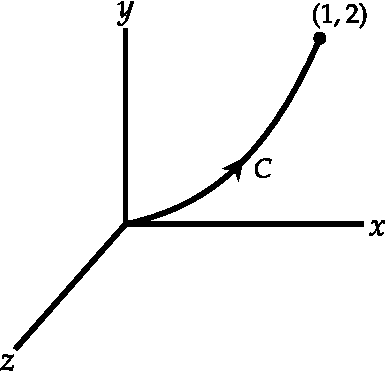
\includegraphics[width=4cm,height=4cm]{VI-Assignment-01}
		\end{center}
	\end{figure}
	\begin{answer}
		The curve lies in $x y$ plane, so, $z=0 . z$ can never be taken as independent variable $z$ is a dependent variable. Now, out of $x$ and $y$, any one variable can be taken as independent.
		Suppose $x$ is taken as independent variable
		\begin{align*}
		 y &=2 x^{2}, d y=4 x d x \\ \vec{F} \cdot d \vec{r} &=3 x y d x-y^{2} d y \\ &=6 x^{3} d x-4 x^{4} \cdot 4 x d x \\ &=\left(6 x^{3}-16 x^{5}\right) d x 
		 \intertext{So, the line integral $\int_{C} \vec{f} \cdot d \vec{r}$ reduces to a definite integral.}
		 \int_{0}^{1}\left(6 x^{3}-16 x^{5}\right) d x&\\
		 &=\left.6 \frac{x^{4}}{4}\right|_{0} ^{1}-\left.16 \frac{x^{6}}{6}\right|_{0} ^{1}\\
		 &=-\frac{7}{6}
		 \intertext{If $y$ is taken as independent variable then $x$ can be expressed in terms of $y$ as}
		 x &=\sqrt{\frac{y}{2}} \\ d x &=\frac{1}{2 \sqrt{2}} \frac{1}{\sqrt{y}} d y \\ \text{So}\quad \vec{f} \cdot d \vec{r} &=3 x y d x-y^{2} d y \\ &=3 y \sqrt{\frac{y}{2}} \cdot \frac{1}{2 \sqrt{2}} \frac{1}{\sqrt{y}} d y-y^{2} d y \\ &=\left(\frac{3}{4} y-y^{2}\right) d y 
		 \intertext{So, the line integral $\int \vec{f} . d \vec{r}$ reduces to a definite integral}
		 \int_{0}^{2}\left(\frac{3}{4} y-y^{2}\right) d y&\\
		 &=\frac{3}{8} y^{2}-\left.\frac{y^{3}}{3}\right|_{0} ^{2}\\
		 &=-\frac{7}{6}\\
		\end{align*}
	\end{answer}
	\item Evaluate $\int_{c} \vec{F} \cdot d \vec{r}$ where $\vec{F}=\left(x^{2}-y^{2}\right) \hat{i}+x y \hat{j}$ and curve $C$ is arc of the curve $y=x^{2}$ from $(0,0)$ to $(2,4)$
	\begin{answer}$\left. \right. $
		\begin{figure}[H]
			\centering
			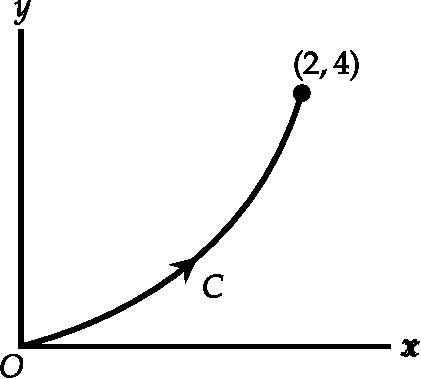
\includegraphics[height=3cm,width=3cm]{VI-Assignment-02}
		\end{figure}
		\begin{align*}
		\vec{F} \cdot d \vec{r}&=\left(x^{2}-y^{2}\right) d x+x y d y
	\intertext{	Taking $x$ as independent variable}
		y=x^{2} & d y=2 x d x \\
		\vec{F} \cdot d \vec{r} & =\left(x^{2}-y^{2}\right) d x+x y d y \\
		& =\left(x^{2}-x^{4}\right) d x+x^{3} \cdot 2 x d x \\
		& =\left(x^{2}+x^{4}\right) d x
		\intertext{So, the line integral $\int \vec{F} \cdot d \vec{r}$ reduces to a definite integral}
		\int_{0}^{2}\left(x^{2}+x^{4}\right) d x&=\frac{x^{3}}{3}+\left.\frac{x^{5}}{5}\right|_{0} ^{2}=\frac{136}{15}
		\intertext{Suppose a force acts on a particle and particles is displaced along a given path $C$. Then work done by the force $\vec{F}$ is given by line integral.}
		W&=\int_{C} \vec{F} \cdot d \vec{r}
		\intertext{The integration is being carried in the sense of displacement.}
		\end{align*}
	\end{answer}
	\item Find the work done when a force
	$$
	\vec{F}=\left(x^{2}-y^{2}+x\right) \hat{i}-(2 x y+y) \hat{j}
	$$
	moves a particle in $x y$ plane from $(0,0)$ to $(1,1)$ along the parabola $y^{2}=x$
	\begin{answer}$\left. \right. $
		\begin{figure}[H]
			\centering
			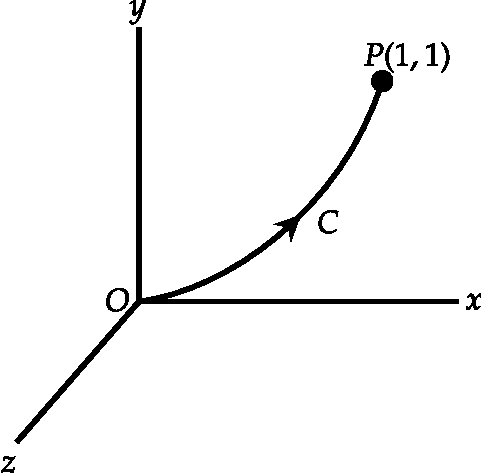
\includegraphics[height=3.5cm,width=3.5cm]{VI-Assignment-03}
		\end{figure}
		\begin{align*}
		\intertext{Here, on the curve $C, y$ can be taken as independent variable and}
	x&=y^{2}, d x=2 y d y
	\intertext{workdone in moving a particle by displacement $d \vec{r}$}
	d W &=\vec{F} \cdot d \vec{r} \\ &=\left(x^{2}-y^{2}+x\right) d x-(2 x y+y) d y \\ &=\left(y^{4}-y^{2}+y^{2}\right) \cdot 2 y d y-\left(2 y^{2} \cdot y+y\right) d y \\ &=\left(2 y^{5}-2 y^{3}-y\right) d y 
	\intertext{Hence, work done is moving a particle from $O$ to $P$ is given by}
	W&=\int_{0}^{1}\left(2 y^{5}-2 y^{3}-y\right) d y=2 \frac{y^{6}}{6}-2 \frac{y^{4}}{4}-\left.\frac{y^{2}}{2}\right|_{0} ^{1}=-\frac{2}{3}
		\end{align*}
	\end{answer}
	\item Evaluate $\oint x d y-y d x$ around a circle $x^{2}+y^{2}=r^{2}$
	\begin{answer}$\left. \right. $
		\begin{figure}[H]
			\centering
			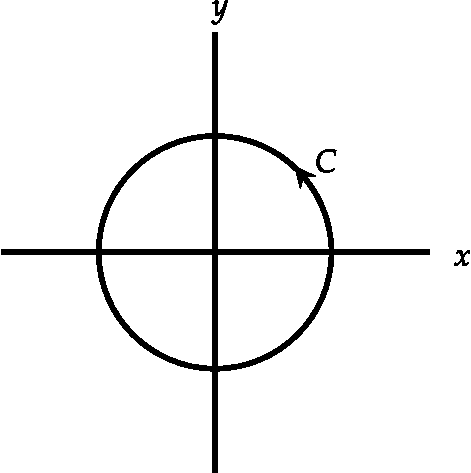
\includegraphics[height=4cm,width=4cm]{VI-Assignment-04}
		\end{figure}
		\begin{align*}
	\intertext{	Let $C$ denotes the circle. The parametric equations of circle is}
		&x=r \cos \theta \\
		&y=r \sin \theta
		\intertext{Here, $x$ and $y$ have been expressed in terms of parameter which varies from 0 to $2 \pi$ as one traverses the circle.}
		x&=r \cos \theta \Rightarrow d x=-r \sin \theta d \theta\\
		y&=r \sin \theta \Rightarrow d y=r \cos \theta d \theta\\
		 x d y-y d x &=r \cos \theta r \cos \theta d \theta-r \sin \theta(-r \sin \theta) d \theta \\ &=r^{2} d \theta \\
		\text{ So,}\quad
		 \oint_{c} x d y-y d x&=r^{2} \oint d \theta \\
		 &=2 \pi r^{2}
		 \intertext{Here, $r$ is a constant, because integral is carried over a circle.}
		\end{align*}
	\end{answer}
	\item  Calculate the work done when a force $\vec{F}=x y \hat{i}+\left(x^{2}+y^{2}\right) \hat{j}$ moves a particle in $x y$ plane from $(1,0)$ to $(3,8)$ along the curve $C, y=x^{2}-1$.
	\begin{answer}$\left. \right. $
		\begin{figure}[H]
			\centering
			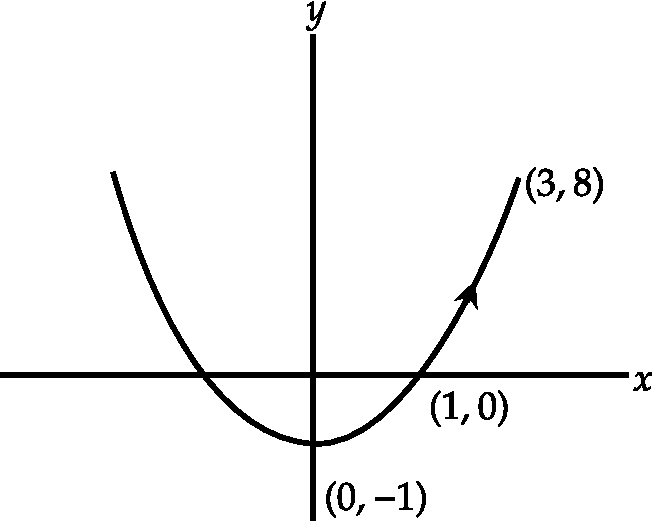
\includegraphics[height=4cm,width=5cm]{VI-Assignment-05}
		\end{figure}
		The curve $C$ is $y=x^{2}-1$. Since, this is quadratic in $x$ and linear in $y$ with no $x y$ terms. This is a parabola. Let us put this parabola in the form
		\begin{align*}
		(x-\alpha)^{2} &=4 a(y-\beta) \\ C:(x-0)^{2} &=(y+1) 
		\intertext{This is a parabola with vertex at $(0,-1)$ and axis parallel to $y$ axis.}
		\intertext{On curve $C$, let us take $x$ as indepedent variable. The dependent variable $y$ can be written in terms of $x$ as}
		 y &=x^{2}-1 \\ d y &=2 x d x 
		 \intertext{work done is moving a particle by displacement $d \vec{r}$}
		  d W &=\vec{F} \cdot d \vec{r} \\ &=x y d x+\left(x^{2}+y^{2}\right) d y \\ &=x\left(x^{2}-1\right) d x+\left(x^{2}+\left(x^{2}-1\right)^{2}\right) 2 x d x \\ &=\left(2 x^{5}-x^{3}+x\right) d x 
		  \intertext{So, work done is moving a particle from $(1,0)$ to $(3,8)$ along a curve $C$.}
		   W &=\int_{c} \vec{F} \cdot d \vec{r}=\int_{1}^{3}\left(2 x^{5}-x^{3}+x\right) d x \\ &=\left.\left(2 \cdot \frac{x^{6}}{6}-\frac{x^{4}}{4}+\frac{x^{2}}{2}\right)\right|_{1} ^{3}=227 
		\end{align*}
	\end{answer}
	\item Evaluate the line integral $\int_{c} \vec{F} \cdot d \vec{r}$ where $\vec{F}=(x+2 y) \hat{i}+(2 y-x) \hat{j}$ and $C$ is curve in $x y$ plane consisting of the straight lines from $(0,0)$ to $(1,0)$ and then to $(3,4)$.
	\begin{answer}
		The curve $C$ consists of two pieces of smooth curves $C_{1}$ and\\ $C_{2}$. $C_{1}$ is straight line from $(0,0)$ to $(1,0)$ ie. $y=0$\\
		$C_{2}$ is straight line from $(1,0)$ to $(3,4)$
		\begin{figure}[H]
			\centering
			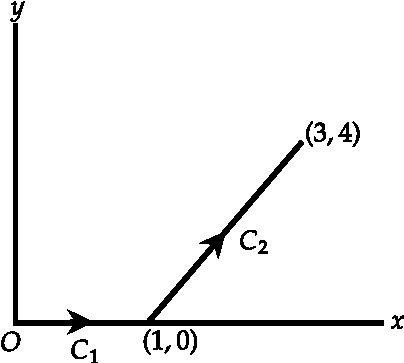
\includegraphics[height=3.5cm,width=3.5cm]{VI-Assignment-06}
		\end{figure}
		\begin{align*}
		\text{i.e}.\qquad \quad y-0&=\left(\frac{4-0}{3-1}\right) \cdot(x-1)\\
		\text{or, }\qquad y&=2 x-2\\
		\text{So, along }C_{1}, y&=0, d y=0 \text{( $x$ is an independent variable )}\\
		\vec{F} \cdot d \vec{r}&=x d x\\
	\text{	Along }C_{2} ; y&=2 x-2, d y=2 d x\text{ (let us take $x$ as independent variables).}\\
		\vec{F} \cdot d \vec{r}&=(x+2 y) d x+(2 y-x) d y\\
	\text{	on }\quad C_{2}, \quad \vec{F} \cdot d \vec{r} &=(x+2(2 x-2)) d x+(2(2 x-2)-x) \cdot 2 d x \\ &=(11 x-12) d x \\
	\text{So,}\quad
	\int_{c} \vec{F} \cdot d \vec{r}&=\int_{c_{1}} \vec{F} \cdot d \vec{r}+\int_{C_{2}} \vec{F} \cdot d \vec{r}\\
	&=\int_{0}^{1} x d x+\int_{1}^{3}(11 x-12) d x\\
	&=\left.\frac{x^{2}}{2}\right|_{0} ^{1}+\left.\left(\frac{11}{2} x^{2}-12 x\right)\right|_{1} ^{3}\\
	&=20.5
		\end{align*}
	\end{answer}
	\item Evaluate $\oint_{C} \vec{F} \cdot d \vec{r}$ where $\vec{F}=\left(x^{2}+y^{2}\right) \hat{i}-2 x y \hat{j}$, where curve $C$ is a rectangle in the $x y$ plane bounded by $y=0, x=a, y=b, x=0$.
	\begin{answer}$\left. \right. $
			\begin{figure}[H]
			\centering
			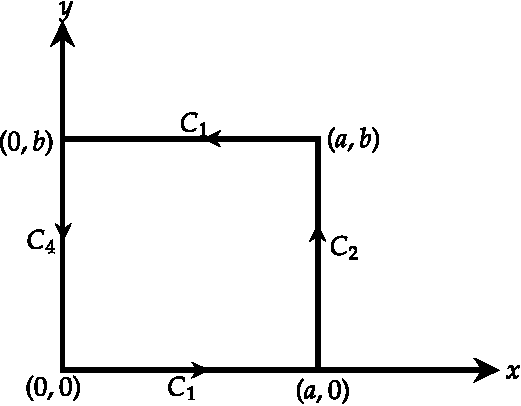
\includegraphics[height=4cm,width=4.6cm]{VI-Assignment-07}
		\end{figure}
		\begin{align*}
		\intertext{The curve $C$ as shown in figure $8.11$ consists of four pieces of smooth curves $C_{1}, C_{2}, C_{3} \& C_{4}$. }
		\vec{F} \cdot d \vec{r}&=\left(x^{2}+y^{2}\right) d x-2 x y d y\\
		\text{On }C_{1}, y&=0, d y=0, \vec{F} . d \vec{r}=x^{2} d x\\
	\text{	On }C_{2}, x&=a, d x=0, \vec{F} \cdot d \vec{r}=-2 a y d y\\
		\text{On }C_{3}, y&=b, d y=0, \vec{F} \cdot d \vec{r}=\left(x^{2}+b^{2}\right) d x\\
		\text{On }C_{4}, x&=0, d x=0, \vec{F} . d \vec{r}=0\\
		\oint \vec{F} \cdot d \vec{r}&=\int_{C_{1}} \vec{F} \cdot d \vec{r}+\int_{C_{2}} \vec{F} \cdot d \vec{r}+\int_{C_{3}} \vec{F} \cdot d \vec{r}+\int_{C_{4}} \vec{F} \cdot d \vec{r}\\
		&=\int_{0}^{a} x^{2} d x+\int_{0}^{b}-2 a y d y+\int_{a}^{0}\left(x^{2}+b^{2}\right) d x+\int_{b}^{0} 0 . d y\\
		&=\left.\frac{x^{3}}{3}\right|_{0} ^{a}+\left[-a y^{2}\right]_{0}^{b}+\left[\frac{x^{3}}{3}+b^{2} x\right]_{a}^{0}\\
		&=\frac{a^{3}}{3}-a b^{2}-\frac{a^{3}}{3}-a b^{2}\\
		&=-2 a b^{2}
		\end{align*}
	\end{answer}
	\item Find the total work done in moving a particles in a force field given by $\vec{F}=3 x y \hat{i}-5 z \hat{j}+10 x \hat{k}$ along the curve $x=t^{2}+1, y=2 t^{2}, z=t^{3}$ from $t=1$ to $t=2$.
	\begin{answer}
		\begin{align*}
		\intertext{On curve $C$, the coordinates $x, y, z$ are expressed in terms of parameter $t$.}
		&x=t^{2}+1, d x=2 t d t \\
		&y=2 t^{2}, d y=4 t d t \\
		&z=t^{3}, d z=3 t^{2} d t\\
		t\text{ varies from }t&=1\text{ to }t=2.\\
		 \vec{F} \cdot d \vec{r} &=3 x y d x-5 z d y+10 x d z \\ &=3\left(t^{2}+1\right) \cdot 2 t^{2} \cdot 2 t d t-5 t^{3} 4 t d t+10\left(t^{2}+1\right) \cdot 3 t^{2} d t \\ &=\left(12 t^{5}+10 t^{4}+12 t^{3}+30 t^{2}\right) d t \\
		 \text{So, total}&\text{ work done,}\\
		  W &=\int_{C} \vec{F} \cdot d \vec{r} \\ &=\int_{1}^{2}\left(12 t^{5}+10 t^{4}+12 t^{3}+30 t^{2}\right) d t \\ &=\left.\left(12 \frac{t^{6}}{6}+10 \frac{t^{5}}{5}+12 \frac{t^{4}}{4}+30 \frac{t^{3}}{3}\right)\right|_{1} ^{2} \\ &=303 
		\end{align*}
	\end{answer}
	\item 
	Find the work done in moving a particle once around a circle $C$ in the $x y$ plane if the circle has a centre at the origin and radius 2 and if the force field $\vec{F}$ is given by
	$$\vec{F}=(2 x-y+2 z) \hat{i}+(x+y-z) \hat{j}+(3 x-2 y-5 z) \hat{k}$$
	\begin{answer}	Equation of circle as shown in figure $8.12$ is written in parametric form as
		\begin{figure}[H]
			\centering
			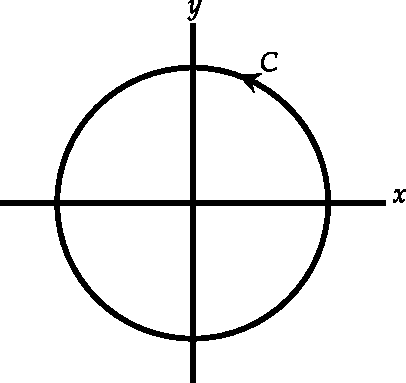
\includegraphics[height=3.8cm,width=4cm]{VI-Assignment-08}
		\end{figure}
		\begin{align*}
		x&=2 \cos \theta \Rightarrow d x=-2 \sin \theta d \theta\\
		y&=2 \sin \theta  \Rightarrow d y=2 \cos \theta d \theta \\ z&=0  \Rightarrow d z=0
		\intertext{$x, y, z$ are expressed in terms of parameter $\theta$.}
	 \vec{F} \cdot d \vec{r}=&(2 x-y+2 z) d x+(x+y-z) d y+(3 x-2 y-5 z) d z \\=&(4 \cos \theta-2 \sin \theta)(-2 \sin \theta) d \theta \\ & \quad+(2 \cos \theta+2 \sin \theta)(6 \cos \theta-4 \sin \theta) .0 \\=&(4-4 \sin \theta \cos \theta) d \theta \\
	 \text{$\theta$ varies from 0 to $2 \pi$}&\\
	 \text{So, total work done}&\\
	  W &=\int_{0}^{2 \pi}(4-4 \sin \theta \cos \theta) d \theta \\ &=4 \theta-\left.2 \sin ^{2} \theta\right|_{0} ^{2 \pi} \\ &=8 \pi 
		\end{align*}
	\end{answer}
	\item If $\vec{F}=\left(3 x^{2}+6 y\right) \hat{i}-14 y z \hat{j}+20 x z^{2} \hat{k}$. Evaluate $\int \vec{F} \cdot d \vec{r}$ where $C$ is a straight line joining $(0,0,0)$ to $(1,1,1)$.
	\begin{answer}
		Equation of straight line joining $(0,0,0)$ to $(1,1,1)$ is given by $\frac{x-0}{1-0}=\frac{y-0}{1-0}=\frac{z-0}{1-0}=t$, where $t$ is parameter.
		\begin{align*}
		\intertext{In parametric form, equation of curve is given by}
		x&=t \Rightarrow d x=d t\\
		y&=t \Rightarrow d y=d t\\
		z&=t \Rightarrow d z=d t
		\intertext{$t$ varies from 0 to 1 .}
		 \vec{F} \cdot d \vec{r} &=\left(3 x^{2}+6 y\right) d x-14 y z d y+20 x z^{2} d z \\ &=\left(20 t^{3}-11 t^{2}+6 t\right) d t \\ \int_{C} \vec{F} \cdot d \vec{r} &=\int_{0}^{1}\left(20 t^{3}-11 t^{2}+6 t\right) d t \\ &=\left.\left(5 t^{4}-\frac{11}{3} t^{3}+3 t^{2}\right)\right|_{0} ^{1} \\ &=\frac{13}{3} 
		\end{align*}
	\end{answer}
	\item  Integrate the function $\vec{F}=x^{2} \hat{i}-x y \hat{j}$ from the point $(0,0)$ to $(1,1)$ along the parabola $y^{2}=x$.
	\begin{answer}
		Here the curve $C$ is parabola $y^{2}=x$ as shown in figure 8.13. On $C, y$ can be taken as independent variable.
		\begin{figure}[H]
			\centering
			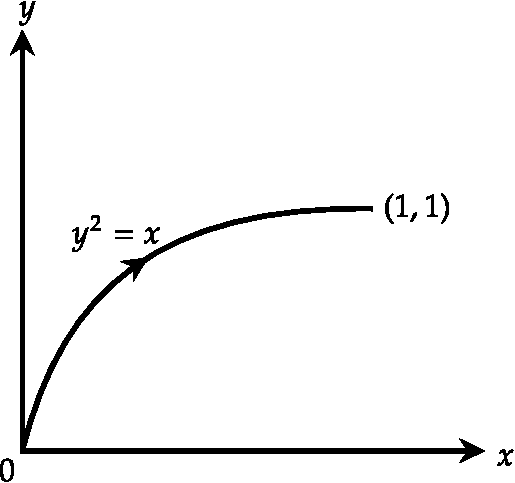
\includegraphics[height=4cm,width=4cm]{VI-Assignment-09}
		\end{figure}
		\begin{align*}
		\intertext{The dependent variable $x$ can be written in terms of $y$ as}
		x&=y^{2}\\
		d x&=2 y d y\\
		 \vec{F} \cdot d \vec{r} &=x^{2} d x-x y d y \\ &=y^{4} \cdot 2 y d y-y^{2} \cdot y d y \\ &=\left(2 y^{5}-y^{3}\right) d y 
		 \text{So, the line integral}\\
		 \int_{C} \vec{F} \cdot d \vec{r} &=\int_{0}^{1}\left(2 y^{5}-y^{3}\right) d y \\ &=\frac{1}{3} y^{6}-\left.\frac{1}{4} y^{4}\right|_{0} ^{1}=\frac{1}{12} 
		\end{align*}
	\end{answer}
\item Find the value of $\int_{C}\left[\left(x+y^{2}\right) d x+\left(x^{2}-y\right) d y\right]$ taken in the counter-clockwise sense along the closed curve $C$ formed by $y^{3}=x^{2}$ and the straight line $y=x$.
\begin{answer}
	The curve $C$ consists of chord $O A$ and curved part $A O$ as shown in figure 8.14.\\
	Equation of $O A$ is $y=x$ and curved part is $y^{3}=x^{2}$.\\
	Along chord $O A, x$ can be taken as independent variable and $y=x$.
	\begin{figure}[H]
		\centering
		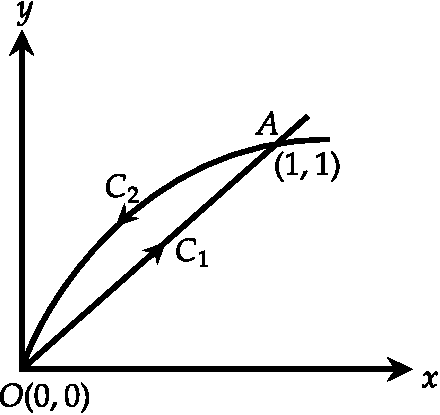
\includegraphics[height=4cm,width=4cm]{VI-Assignment-10}
	\end{figure}
	\begin{align*}
	 \vec{F} \cdot d \vec{r} &=\left(x+y^{2}\right) d x+\left(x^{2}-y\right) d y \\ &=\left(x+x^{2}\right) d x+\left(x^{2}-x\right) d x \\ &=2 x^{2} d x 
	 \intertext{Along $O A, x$ varies from 0 to 1 . On curved part $A O$, let $y$ be taken as independent variable $\&$ dependent variable $x$ can be put as}
	 x&=y^{3 / 2}, d x=\frac{3}{2} y^{1 / 2} d y\\
	  \vec{F} \cdot d \vec{r} &=\left(x+y^{2}\right) d x+\left(x^{2}-y\right) d y \\ &=\left(y^{3 / 2}+y^{2}\right) \frac{3}{2} y^{1 / 2} d y+\left(y^{3}-y\right) d y \\ &=\left(y^{3}+\frac{3}{2} y^{5 / 2}+\frac{3}{2} y^{2}-y\right) d y \\
	  \text{$y$ varies from 1 to $0 .$}\\
	  \oint_{C} \vec{F} \cdot d \vec{r}&=\int_{C_{1}} \vec{F} \cdot d \vec{r}+\int_{C_{2}} \vec{F} \cdot d \vec{r}\\
	  &=\int_{0}^{1} 2 x^{2} d x+\int_{1}^{0}\left(y^{3}+\frac{3}{2} y^{5 / 2}+\frac{3}{2} y^{2}-y\right) d y\\
	  &=\left.\frac{2}{3} x^{3}\right|_{0} ^{1}+\frac{1}{4} y^{4}+\frac{3}{7} y^{7 / 2}+\frac{1}{2} y^{3}-\left.\frac{1}{2} y^{2}\right|_{1} ^{0}\\
	  &=-\frac{1}{84}
	  \intertext{
	  	Note:- If the integral is carried out in clockwise direction. The answer will differ only in sign. $\oint_{C} \vec{F} \cdot d \vec{r}$ in clockwise direction $=\frac{1}{84}$}
	\end{align*}
\end{answer}
\item Calculate $\int_{C} \vec{F} \cdot d \vec{r}$ where $\vec{F}=\frac{y^{2}}{x^{2}+y^{2}} \hat{i}-\frac{x^{2}}{x^{2}+y^{2}} \hat{j}$, where $C$ is the semi-circle $y=\sqrt{a^{2}-x^{2}}$.
\begin{answer}$\left. \right. $
	\begin{figure}[H]
		\centering
		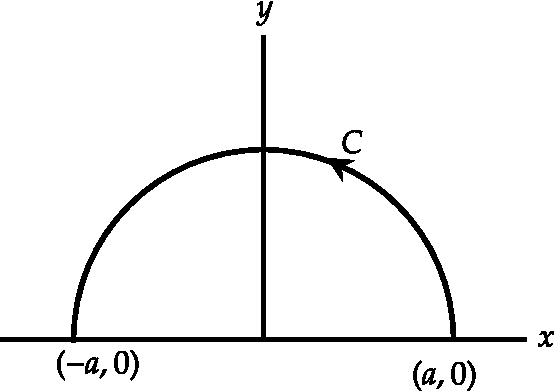
\includegraphics[height=3.5cm,width=5cm]{VI-Assignment-11}
	\end{figure}
	The curve $C$ shown in Figure $8.15$ is the semi-circle
	\begin{align*}
	y&=\sqrt{a^{2}-x^{2}}
	\intertext{The equation can be written in parametric form as}
	x&=a \cos \theta \Rightarrow d x=-a \sin \theta d \theta\\
	y&=a \sin \theta \Rightarrow d y=a \cos \theta d \theta
	\intertext{$\theta$ varies from 0 to $\pi$.}
	\vec{F} \cdot d \vec{r}&=\frac{y^{2} d x-x^{2} d y}{x^{2}+y^{2}}\\
	&=\frac{a^{2} \sin ^{2} \theta(-a \sin \theta) d \theta-\left(a^{2} \cos ^{2} \theta\right) a \cos \theta d \theta}{a^{2}}\\
	&=-a\left(\sin ^{3} \theta+\cos ^{3} \theta\right) d \theta\\
	\int_{C} \vec{F} \cdot d \vec{r}&=-a \int_{0}^{\pi}\left(\sin ^{3} \theta+\cos ^{3} \theta\right) d \theta\\
	&=-a \int_{0}^{\pi} \sin ^{3} \theta d \theta-a \int_{0}^{\pi} \cos ^{3} \theta d \theta\\
	&=-2 a \int_{0}^{\pi / 2} \sin ^{3} \theta d \theta-0\left(\right.
	\text{ Since, }\left.\int_{0}^{\pi} \cos ^{3} \theta d \theta=0\right)\\
	&=-2 a \frac{\sqrt{2} \sqrt{1 / 2}}{2 \cdot \sqrt{5 / 2}}\\
	&=-\frac{4 a}{3}
	\end{align*}
\end{answer}
\item Evaluate $\int_{C} \frac{d x}{x+y}$ where $C$ is the curve $y^{2}=4 a x$ from $(0,0)$ to $(4 a, 4 a)$.
\begin{answer}
	The equation of curve (as shown in the figure 8.16) can be written in parametric form as
	\begin{figure}[H]
		\centering
		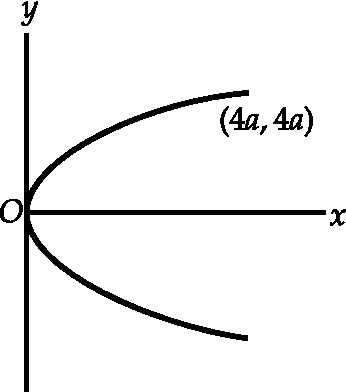
\includegraphics[height=3.7cm,width=3.5cm]{VI-Assignment-12}
	\end{figure}
	\begin{align*}
	x&=a t^{2} \Rightarrow d x=2 a t d t\\
	y&=2 a t \Rightarrow d y=2 a d t
	\intertext{Parameter, $t$ varies from 0 to 2 .}\\
	\text{The integral}\\
	 \int_{0} \frac{d x}{x+y} &=\int_{0}^{2} \frac{2 a t d t}{a t^{2}+2 a t}=2 \int_{0}^{2} \frac{d t}{t+2}=\left.2 \log (t+2)\right|_{0} ^{2} \\ &=2 \log 2 
	\end{align*}
\end{answer}
\item Evaluate $\int_{C}(y d x-x d y)$, where $C$ is arc of cycloid $x=2(\theta-\sin \theta), y=2(1-\cos \theta)$ joining the points $(0,0)$ and $(4 \pi, 0)$.
\begin{answer}
		The parametric equation of curve $C$ as shown in figure $8.17$ is given as
		\begin{figure}[H]
			\centering
			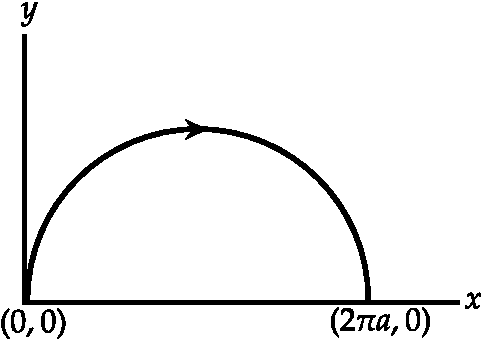
\includegraphics[height=3.5cm,width=5cm]{VI-Assignment-13}
		\end{figure}
	\begin{align*}
	x&=2(\theta-\sin \theta) \Rightarrow d x=2(1-\cos \theta) d \theta \\
	y&=2(1-\cos \theta) \Rightarrow d y=2 \sin \theta d \theta
	\intertext{$\theta$ is the parameter since $(x, y)$ varies from $(0,0)$ to $(4 \pi, 0)$. So, $\theta$ will vary from 0 to $2 \pi$.
		The integrand $y d x-x d y$}
	&=2(1-\cos \theta) \cdot 2(1-\cos \theta) d \theta-2(\theta-\sin \theta) \cdot 2 \sin \theta d \theta\\
	&=4(2-2 \cos \theta-\theta \sin \theta)\\
\text{	So,}\quad
	\int_{C} y d x-x d y&=4 \int_{0}^{2 \pi}(2-2 \cos \theta-\theta \sin \theta) d \theta\\
	&=8 \int_{0}^{2 \pi} d \theta-8 \int_{0}^{2 \pi} \cos \theta d \theta-4 \int_{0}^{2 \pi} \theta \sin \theta d \theta\\
	&=16 \pi-8[\sin \theta]_{0}^{2 \pi}-4[-\theta \cos \theta+\sin \theta]_{0}^{2 \pi}\\
	&=24 \pi
	\end{align*}
\end{answer}
\item Evaluate $\int_{C} \vec{F} \cdot d \vec{r}$ where $\vec{F}=(2 a-y) \hat{i}-(a-y) \hat{j}$ where $C$ is the arc of the cycloid $x=a(\theta-\sin \theta)$, $y=a(1-\cos \theta)$ from $(0,0)$ to $(2 \pi a, 0)$.
\begin{answer}
	The equation of cycloid is written in parametric form as
	\begin{align*}
	x&=a(\theta-\sin \theta) \Rightarrow d x=a(1-\cos \theta) d \theta\\
	y&=a(1-\cos \theta) \Rightarrow d y=a \sin \theta d \theta
	\intertext{where $\theta$ is the parameter varying from 0 to $2 \pi$.}
\text{	On $C:$}
	\vec{F} \cdot d \vec{r} &=(2 a-y) d x-(a-y) d y \\
	&=a(1+\cos \theta) \cdot a(1-\cos \theta) d \theta-a \cos \theta \cdot a \sin \theta d \theta \\
	&=a^{2}\left(1-\cos ^{2} \theta-\sin \theta \cos \theta\right) d \theta
	\intertext{So, the line integral}
	 \int_{C} \vec{F} \cdot d \vec{r} &=a^{2} \int_{0}^{2 \pi}\left(1-\cos ^{2} \theta-\sin \theta \cos \theta\right) d \theta \\ &=a^{2} \int_{0}^{2 \pi} d \theta-a^{2} \int_{0}^{2 \pi} \cos ^{2} \theta d \theta-a^{2} \int_{0}^{2 \pi} \sin \theta \cos \theta d \theta \\ &=\pi a^{2} 
	\end{align*}
\end{answer}
\item Evaluate $\int_{C} \frac{x^{2} d y-y^{2} d x}{x^{5 / 3}+y^{5 / 3}}$
where $C$ is the quarter of the astroid $x=a \cos ^{3} t, y=a \sin ^{3} t$ from the point $(a, 0)$ to the point $(0, a)$.
\begin{answer}
	The parametric equation of the astroid as shown in figure $8.18$ is given as
	\begin{figure}[H]
		\centering
		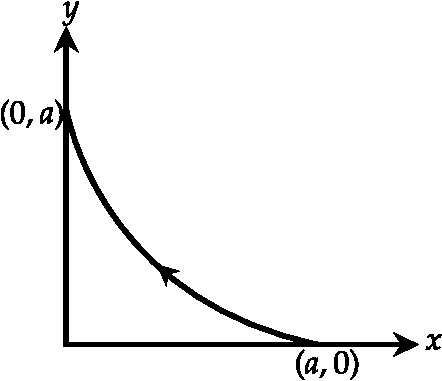
\includegraphics[height=3.5cm,width=4cm]{VI-Assignment-14}
	\end{figure}
	\begin{align*}
	x&=a \cos ^{3} t \Rightarrow d x=-3 a \cos ^{2} t \sin t d t\\
	y&=a \sin ^{3} t \Rightarrow d y=3 a \sin ^{2} t \cos t d t
	\intertext{$(x, y)$ varies from $(a, 0)$ to $(0, a)$.}
	\intertext{So, $t$ varies from 0 to $\pi / 2$.}
	\text{The integrand }&\frac{x^{2} d y-y^{2} d x}{x^{5 / 3}+y^{5 / 3}}\\
	&=\frac{a^{2} \cos ^{6} t\left(3 a \sin ^{2} t \cos t\right) d t-\left(a^{2} \sin ^{6} t\right) \cdot\left(-3 a \cos ^{2} t \sin t\right) d t}{a^{5 / 3}\left(\cos ^{5} t+\sin ^{5} t\right)}\\
	&=3 a^{4 / 3} \sin ^{2} t \cos ^{2} t d t
	\intertext{The line integral reduces to}
	3 a^{4 / 3} \int_{0}^{\pi / 2} \sin ^{2} t \cos ^{2} t d t&=3 a^{4 / 3} \frac{\sqrt{3 / 2 / 3 / 2}}{2 \sqrt{3}}=\frac{3 \pi a^{4 / 3}}{16}
	\end{align*}
\end{answer}
\item Find the value of $\int_{c}\left(x^{2}+y^{2}\right) d y$ taken in the counter clockwise sense along the quadrilateral with vertices $(0,0),(2,0),(4,4),(0,4)$.
\begin{answer}
	The quadirlateral as shown in Figure $8.19$ consists of four pieces of smooth curves $A B, B C, C D $\&$ D A$.
	\begin{figure}[H]
		\centering
		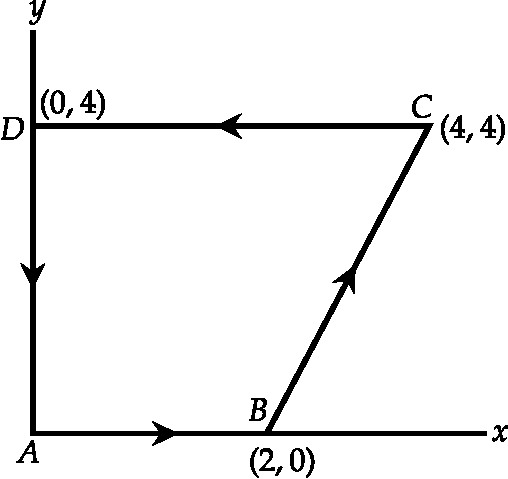
\includegraphics[height=4cm,width=4cm]{VI-Assignment-15}
	\end{figure}
	\begin{align*}
	\text{On }A B, y&=0, d y=0,\left(x^{2}+y^{2}\right) d y=0\\
	 y &=2 x-4, d y=2 d x \\\left(x^{2}+y^{2}\right) d y &=\left(x^{2}+(2 x-4)^{2}\right) 2 d x \\ &=\left(10 x^{2}-32 x+32\right) d x \\
	 \text{$x$ varies from 2 to 4}\\
	 \text{On CD, }y&=4, d y=0\\
	 \left(x^{2}+y^{2}\right) d y=0\\
	 \text { On  D A, }x&=0, d x=0\\
	 \left(x^{2}+y^{2}\right) d y&=y^{2} d y\\
	 \text{$y$ varies from 4 to 0}\\
	\text{ So, the line integral}\\
	 \int_{C}\left(x^{2}+y^{2}\right) d y &=\int_{A B}\left(x^{2}+y^{2}\right) d y+\int_{B C}\left(x^{2}+y^{2}\right) d y+\int_{C D}\left(x^{2}+y^{2}\right) d y+\int_{D A}\left(x^{2}+y^{2}\right) d y \\ &=0+\int_{2}^{4}\left(10 x^{2}-32 x+32\right) d x+0+\int_{4}^{0} y^{2} d y \\ &=\left.\left(\frac{10}{3} x^{3}-16 x^{2}+32 x\right)\right|_{2} ^{4}+\left.\frac{y^{3}}{3}\right|_{4} ^{0} \\ &=\frac{112}{3} 
	\end{align*}
\end{answer}
\item  Evaluate $\int_{C} x y^{2} d y-x^{2} y d x$ taken in the counter clockwise sense along the cardioid $r=a(1+\cos \theta)$
\begin{answer}
	The curve $C$ as shown in figure $8.20$ cardiod whose equation is
	\begin{figure}[H]
		\centering
		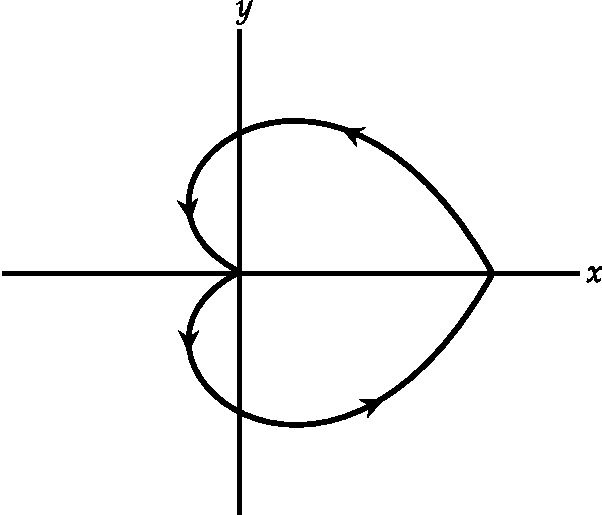
\includegraphics[height=4cm,width=5cm]{VI-Assignment-16}
	\end{figure}
	\begin{align*}
	r&=a(1+\cos \theta)\\
	x&=r \cos \theta=a(1+\cos \theta) \cos \theta=a\left(\cos \theta+\cos ^{2} \theta\right)\\
	d x&=a(-\sin \theta-2 \cos \theta \sin \theta) d \theta\\
	y &=r \sin \theta=a(1+\cos \theta) \sin \theta=a(\sin \theta+\sin \theta \cos \theta) \\ d y &=a\left(\cos \theta+\cos ^{2} \theta-\sin ^{2} \theta\right) d \theta \\
	\text{The integrand}&\\
	\left(x y^{2} d y-x^{2} y d x\right)&\\
	&=r^{3} \cos \theta \sin ^{2} \theta a\left(\cos \theta+\cos ^{2} \theta-\sin ^{2} \theta\right) d \theta\\
	&\quad \quad-r^{3} \cos ^{2} \theta \sin \theta a(\sin \theta-2 \cos \theta \sin \theta) d \theta\\
	&=a r^{2} \cos \theta \sin ^{2} \theta\left(\cos \theta+\cos ^{2} \theta-\sin ^{2} \theta+\cos \theta+2 \cos ^{2} \theta\right) d \theta\\
	&=a^{4}(1+\cos \theta)^{3} \cos \theta \sin ^{2} \theta\left(4 \cos ^{2} \theta+2 \cos \theta-1\right) d \theta\\
	&=a^{4}\left[\cos ^{6} \theta \sin ^{2} \theta+14 \cos ^{5} \theta \sin ^{2} \theta+17 \cos ^{4} \theta \sin ^{2} \theta\right.\\
	&\left.\quad+7 \cos ^{3} \theta \sin ^{2} \theta-\cos ^{2} \theta \sin ^{2} \theta-\cos \theta \sin ^{2} \theta\right]\\
	\text{The line integral}&\\
	\oint\left(x y^{2} d y-x^{2} y d x\right)&\\
	&=a^{4} \int_{0}^{2 \pi}\left(\cos ^{6} \theta \sin ^{2} \theta+14 \cos ^{5} \theta \sin ^{2} \theta+17 \cos ^{4} \theta \sin ^{2} \theta+7 \cos ^{3} \theta \sin ^{2} \theta\right.\\
	&\quad \left.-\cos ^{2} \theta \sin ^{2} \theta-\cos \theta \sin ^{2} \theta\right) d \theta\\
	&=\frac{35}{16} a^{4} \pi
	\end{align*}
\end{answer}
\item A particle moves counterclockwise along the curve $3 x^{2}+y^{2}=3$ from $(1,0)$ to a point $P$, under the action of the force
$$
\vec{F}(x, y)=\frac{x}{y} \hat{i}+\frac{y}{x} \hat{j} .
$$
Prove that there are two possible locations of $P$ such that the work done by $\vec{F}$ is 1 .
\begin{answer}$\left. \right. $
	\begin{figure}[H]
		\centering
		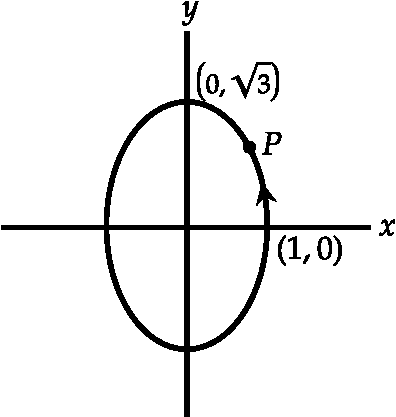
\includegraphics[height=4.5cm,width=4cm]{VI-Assignment-17}
	\end{figure}
	\begin{align*}
	\frac{x^{2}}{1}+\frac{y^{2}}{3}&=1
	\intertext{Point on ellipse is represented as}
	(\cos \theta, \sqrt{3} \sin \theta)&\\
	 \int \vec{F} \cdot d \vec{r} &=\int\left(\frac{x}{y} \hat{i}+\frac{y}{x} \hat{j}\right) \cdot(d x \hat{i}+d y \hat{j}) \\ &=\int \frac{x}{y} d x+\frac{y}{x} d y \\ &=\int_{0}^{\theta} \frac{\cos \theta}{\sqrt{3} \sin \theta}(-\sin \theta) d \theta+\frac{\sqrt{3} \sin \theta}{\cos \theta} \cdot \sqrt{3} \cos \theta d \theta \\ &=\int_{0}^{\theta}\left(-\frac{1}{\sqrt{3}} \cos \theta+3 \sin \theta\right) d \theta \\ &=-\frac{1}{\sqrt{3}} \sin \theta-\left.3 \cos \theta\right|_{0} ^{\theta} \\ &=-\frac{1}{\sqrt{3}} \sin \theta-3 \cos \theta+3 
	 \intertext{Work done in equal to 1}
	 \mathrm{So},&-\frac{1}{\sqrt{3}} \sin \theta-3 \cos \theta+3=1\\
	 \Rightarrow &\quad \frac{1}{\sqrt{3}} \sin \theta+3 \cos \theta=2\\
	 \Rightarrow &\quad\left(\frac{1}{\sqrt{3}} \sin \theta\right)^{2}=(2-3 \cos \theta)^{2}\\
	 \Rightarrow &\quad \frac{1}{3} \sin ^{2} \theta=4+9 \cos ^{2} \theta-12 \cos \theta\\
	 \Rightarrow &\quad 28 \cos ^{2} \theta-36 \cos \theta+11=0\\
	 \Rightarrow &\quad(2 \cos \theta-1)(14 \cos \theta-11)=0\\
	 \quad \cos \theta&=\frac{1}{2}, \frac{11}{14}
	 \intertext{So, there are two value of $\theta$ i.e., two possible location of $P$ such that the work done by $\vec{F}$ is 1 .}
	\end{align*}
\end{answer}
\item Find the circulation of the field
$$
\vec{F}=-x^{2} y \hat{i}+x y^{2} \hat{j}+\left(y^{3}-x^{3}\right) \hat{k}
$$
around the curve $C$, where $C$ is the intersection of the sphere $x^{2}+y^{2}+z^{2}=25$ and the plane $z=3$. The orientation of the curve $C$ is counterclockwise when viewed from above.
\begin{answer}$\left. \right. $
	\begin{figure}[H]
		\centering
		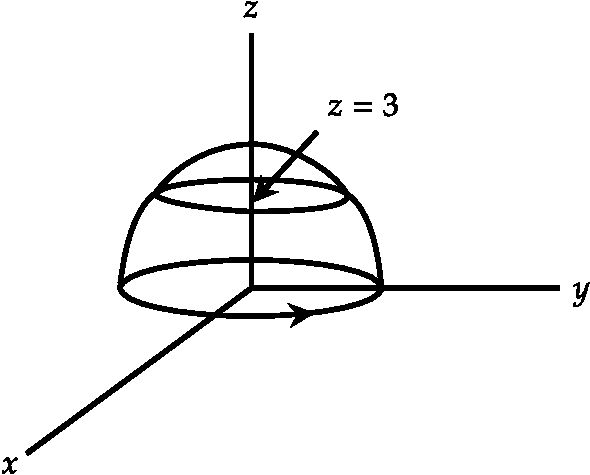
\includegraphics[height=4cm,width=5.2cm]{VI-Assignment-18}
	\end{figure}
	\begin{align*}
	\vec{F}&=-x^{2} y \hat{i}+x y^{2} \hat{j}+\left(y^{3}-x^{3}\right) \hat{k}
\intertext{	$C$ is the curve of intersection of surfaces}
	x^{2}+y^{2}+z^{2}&=25, z=3\\
	\text{So, }\quad x^{2}+y^{2}&=16\\
	\vec{F} \cdot d \vec{r}&=x^{2} y d x+x y^{2} d y+\left(y^{3}-x^{3}\right) d z\\
	\text{For curve }C, z&=3, d z=0\\
	\oint \vec{F} \cdot d \vec{r}&=\int-x^{2} y d x+x y^{2} d y\\
	\text{Let }x&=4 \cos \theta, y=4 \sin \theta\\
	 \oint \vec{F} \cdot d \vec{r} &=\int_{0}^{2 \pi}\left(256 \cos ^{2} \theta \sin ^{2} \theta d \theta+256 \cos ^{2} \theta \sin ^{2} \theta\right) d \theta \\ &=512 \int_{0}^{2 \pi} \sin ^{2} \theta \cos ^{2} \theta d \theta \\ &=512 \times 4 \int_{0}^{\pi / 2} \sin ^{2} \theta \cos ^{2} \theta d \theta \\ &=2048 \frac{\sqrt{3 / 2} \sqrt{3 / 2}}{2 \sqrt{3}}=128 \pi 
	\end{align*}
\end{answer}
\item If $\phi=2 x^{2} y z, \vec{F}=x y \hat{i}-z^{2} y \hat{j}+x^{2} \hat{k}$ and $C$ is the curve $x=2 t, y=t^{2}, z=t^{3}$ from $t=0$ and $t=1$. Evaluate the line integrals (a) $\int_{C} \phi d \vec{r}$ (b) $\int_{C} \vec{F} \times d \vec{r}$.
\begin{answer}
	\begin{align*}
\text{	(a)\quad Along }C, \phi&=2 x^{2} y z=2(2 t)^{2} \cdot t^{2} \cdot t^{3}=8 t^{7}\\
	\vec{r} &=x \hat{i}+y \hat{j}+z \hat{k} \\
	&=2 t \hat{i}+t^{2} \hat{j}+t^{3} \hat{k} \\
	d \vec{r} &=\left(2 \hat{i}+2 \hat{j}+3 t^{2} \hat{k}\right) d t \\
	\int_{C} \phi d \vec{r} &=\int_{0}^{1} 8 t^{7}\left(2 \hat{i}+2 t \hat{j}+3 t^{2} \hat{k}\right) d t \\
	&=\hat{i}_{0}^{1} 16 t^{7} d t+\hat{j}_{0}^{1} 16 t^{8} d t+\hat{k} \int_{0}^{1} 24 t^{9} d t \\
	&=2 \hat{i}+\frac{16}{9} \hat{j}+\frac{12}{5} \hat{k}\\\\
	\text{(b)\quad Along }C, \vec{F}&=x y \hat{i}-z^{2} y \hat{j}+x^{2} \hat{k}\\
	&=2 t^{3} \hat{i}-t^{8} \hat{j}+4 t^{2} \hat{k} \\
	\vec{F} \times d \vec{r} &=\left(2 t^{3} \hat{i}-t^{8} \hat{j}+4 t^{2} \hat{k}\right) \times\left(2 \hat{i}+2 t \hat{j}+3 t^{2} \hat{k}\right) \\
	&=\left|\begin{array}{ccc}
	\hat{i} & \hat{j} & \hat{k} \\
	2 t^{3} & -t^{8} & 4 t^{2} \\
	2 & 2 t & 3 t^{2}
	\end{array}\right| \\
	&=\left(-3 t^{10}-8 t^{3}\right) \hat{i}+\left(8 t^{2}-6 t^{5}\right) \hat{j}+\left(4 t^{4}+2 t^{8}\right) \hat{k} \\
	\int_{C} \vec{F} \times d \vec{r} &=\hat{i}_{0}^{1}\left(-3 t^{10}-8 t^{3}\right) d t+\hat{j} \int_{0}^{1}\left(8 t^{2}-6 t^{5}\right) d t+\hat{k} \int_{0}^{1}\left(4 t^{4}+2 t^{8}\right) d t \\
	&=-\frac{47}{11} \hat{i}+\frac{5}{3} \hat{j}+\frac{46}{45} \hat{k}
	\end{align*}
\end{answer}
\item Find the work done in moving the particle once round the ellipse $\frac{x^{2}}{25}+\frac{y^{2}}{16}=1, z=0$ under the field of force given by $\vec{F}=(2 x+y+z) \hat{i}+\left(x+y-z^{2}\right) \hat{j}+(3 x-2 y+4 z) \hat{k}$.
\begin{answer}
		Work done moving the particle by distance $d r$
		\begin{figure}[H]
			\centering
			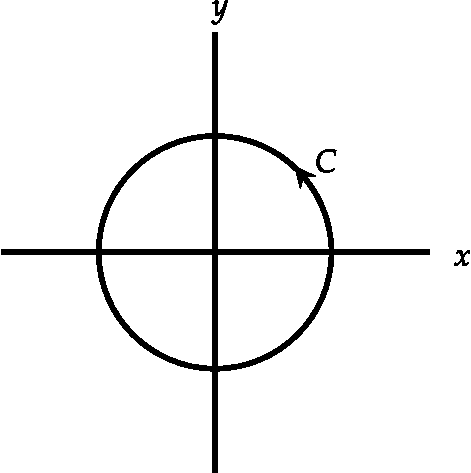
\includegraphics[height=3.5cm,width=3.5cm]{VI-Assignment-19}
		\end{figure}
	\begin{align*}
	\vec{F} \cdot d \vec{r}&=(2 x+y+z) d x+\left(x+y-z^{2}\right) d y+(3 x-2 y+4 z) d z\\
	\text{The curve $C$ is ellipse }&\frac{x^{2}}{25}+\frac{y^{2}}{16}=1\\
\text{	The equation  }&\text{of ellipse is given by}x=5 \cos \theta, y=4 \sin \theta, z=0\\
d x &=-5 \sin \theta d \theta \\ d y &=4 \cos \theta d \theta \\ d z &=0 \\ \vec{F} \cdot d \vec{r} &=(10 \cos \theta+4 \sin \theta)(-5 \sin \theta) d \theta+(5 \cos \theta+4 \sin \theta) 4 \cos \theta d \theta \\ &=\left(-34 \sin \theta \cos \theta+20 \cos ^{2} \theta-20 \sin ^{2} \theta\right) d \theta 
\intertext{On $C, \theta$ varies from 0 to $2 \pi$}
\intertext{So, work done in moving a particle around the ellipse}
\text{So, }\quad W&=\oint \vec{F} \cdot d \vec{r}\\
&=\int_{0}^{2 \pi}\left(-34 \sin \theta \cos \theta+20 \cos ^{2} \theta-20 \sin ^{2} \theta\right) d \theta\\
&=-34 \int_{0}^{2 \pi} \sin \theta \cos \theta d \theta+20 \int_{0}^{2 \pi} \cos ^{2} \theta d \theta-20 \int_{0}^{2 \pi} \sin ^{2} \theta d \theta \\
&=0
	\end{align*}
\end{answer}
\item Evaluate $\int_{C} \vec{F} \cdot d \vec{r}$ where $\vec{F}=c\left[-3 a \sin ^{2} \theta \cos \theta \hat{i}+a\left(2 \sin \theta-3 \sin ^{2} \theta\right) \hat{j}+b \sin 2 \theta \hat{k}\right]$ and the curve $C$ is given by $\vec{r}=a \cos \theta \hat{i}+a \sin \theta \hat{j}+b \theta \hat{k}, \theta$ varying from $\frac{\pi}{4}$ to $\frac{\pi}{2}$.
\begin{answer}
	\begin{align*}
	 \vec{r} &=a \cos \theta \hat{i}+a \sin \theta \hat{j}+b \theta \hat{k} \\ d \vec{r} &=(-a \sin \theta \hat{i}+a \cos \theta \hat{j}+b \hat{k}) d \theta \\ \vec{F} \cdot d \vec{r} &=c\left[3 a^{2} \sin ^{3} \theta \cos \theta+a^{2}\left(2 \sin \theta-3 \sin ^{2} \theta\right) \cos \theta+b^{2} \sin 2 \theta\right] d \theta 
	 \intertext{The line integral}
	  \int_{C} \vec{F} \cdot d \vec{r} &=3 a^{2} c \int_{\pi / 4}^{\pi / 2} \sin ^{3} \theta \cos \theta d \theta+a^{2} c \int_{\pi / 4}^{\pi / 2}\left(2 \sin \theta-3 \sin ^{2} \theta\right) \cos \theta d \theta+b^{2} c \int_{\pi / 4}^{\pi / 2} \sin 2 \theta d \theta \\ &=3 a^{2} c\left[\frac{\sin ^{4} \theta}{4}\right]_{\pi / 4}^{\pi / 2}+a^{2} c\left[\sin ^{2} \theta-\sin ^{3} \theta\right]_{\pi / 4}^{\pi / 2}-\frac{b^{2} c}{2}[\cos 2 \theta]_{\pi / 4}^{\pi / 2} \\ &=\frac{9}{16} a^{2} c+a^{2} c\left[\frac{1}{2}-\frac{1}{2 \sqrt{2}}\right]+\frac{b^{2} c}{2} \\ &=\left(\frac{17}{16}-\frac{1}{2 \sqrt{2}}\right) a^{2} c+\frac{b^{2} c}{2} 
	\end{align*}
\end{answer}
\end{enumerate}
\section{Green's Theorem}
\begin{enumerate}
	\item Verify Green's theorem in the place for $\oint_{C}\left(x y+x^{2}\right) d x+x^{2} d y$ where $C$ is the closed curve of the region 
	bounded by $y=x$ and $x^{2}=4 a y$.
	\begin{figure}[H]
		\centering
		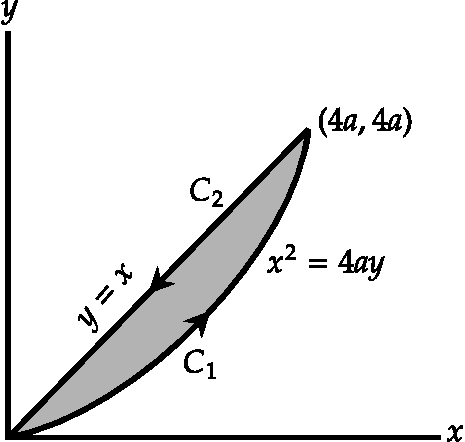
\includegraphics[height=4cm,width=4.5cm]{GT-Assignment-01}
	\end{figure}
	\begin{answer}
		\begin{align*}
	\text{	Here }M d x&+N d y\\
		&=\left(x y+x^{2}\right) d x+x^{2} d y \\
		M&=x y+x^{2} \Rightarrow \frac{\partial M}{\partial y}=x \\
		N&=x^{2} \quad \Rightarrow \frac{\partial N}{\partial x}=2 x
		\intertext{Let us first evaluate the double integral over Region $R$ bounded by $x^{2}=4 a y$ (curve $\left.C_{1}\right) \& y=x$ (curve $C_{2}$ ) as}
	 \iint\left(\frac{\partial N}{\partial x}-\frac{\partial M}{\partial y}\right) d x d y &=\int_{0}^{4 a} \int_{x^{2} / 4 a}^{x} x d y d x \\ &=\int_{0}^{4 a} x\left(x-\frac{x^{2}}{4 a}\right) d x=\frac{x^{3}}{3}-\left.\frac{x^{4}}{16 a}\right|_{0} ^{4 a}=\frac{16 a^{3}}{3} 
	 \intertext{Now let us evaluate the line integral $\oint M d x+N d y$ on closed curve $C$. The curve $C$ is a piecewise smooth curve consisting of $C_{1}$ and $C_{2}$.}
	\text{ On }C_{1}, y&=\frac{x^{2}}{4 a}\quad 
	 d y=\frac{x}{2 a} d x\\
	 M d x+N d y &=\left(x y+x^{2}\right) d x+x^{2} d y \\ &=\left(\frac{x^{3}}{4 a}+x^{2}\right) d x+x^{2} \frac{x}{2 a} d x \\ &=\left(\frac{3}{4} \cdot \frac{x^{3}}{a}+x^{2}\right) d x 
	 \intertext{$x$ varies from 0 to $4 a$ on $C_{1}$}
	\text{ So,}
	 \int_{C_{1}} M d x+N d y&=\int_{0}^{4 a}\left(\frac{3 x^{3}}{4 a}+x^{2}\right) d x\\
	 &=\frac{3}{16 a} x^{4}+\left.\frac{x^{3}}{3}\right|_{0} ^{4 a}\\
	 &=8 a^{3}+\frac{64 a^{3}}{3}=\frac{208 a^{3}}{3}\\
	 \text{On }C_{2}, \quad y&=x, d y=d x\\
	 M d x+N d y &=\left(x y+x^{2}\right) d x+x^{2} d y \\ &=3 x^{2} d x 
	 \intertext{$x$ varies from $4 a$ to 0 .}
	\text{ So,}
	 \int_{C_{2}} M d x+N d y&=\int_{4 a}^{0} 3 x^{2} d x\\
	 &=\left.x^{3}\right|_{4 a} ^{0}=-64 a^{3}\\
	  \text{so, }\int_{C} M d x+N d y &=\int_{C_{1}} M d x+N d y+\int_{C_{2}} M d x+N d y \\ &=\frac{208}{3} a^{3}-64 a^{3}=\frac{16}{3} a^{3} \\
	 \text{ Since, }
	  \iint_{R}\left(\frac{\partial N}{\partial x}-\frac{\partial M}{\partial y}\right) d x d y&=\oint_{C} M d x+N d y
	 \intertext{ So, Green's theorem is verified.}
		\end{align*}
	\end{answer}
	\item 	Apply Green's theorem in the plane to evaluate $\oint\{(y-\sin x) d x+\cos x d y\}$ where $C$ is the triangle enclosed by the lines $y=0, x=\pi, \pi y=2 x$.
	\begin{answer}$\left. \right. $
		\begin{figure}[H]
			\centering
			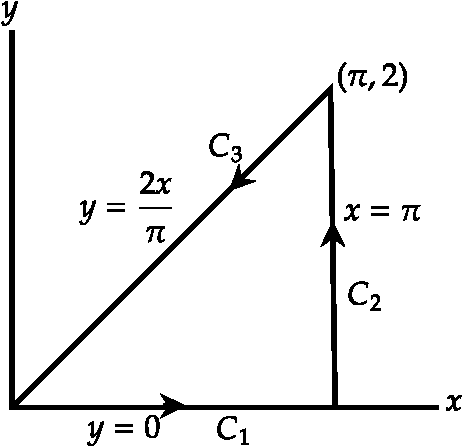
\includegraphics[height=4cm,width=4cm]{GT-Assignment-06}
		\end{figure}
		\begin{align*}
	\text{	Here, }\quad M d x+N d y&=(y-\sin x) d x+\cos x d y\\
	\text{So, }\quad M&=y-\sin x, \quad \frac{\partial M}{\partial y}=1\\
	N&=\cos x, \quad \frac{\partial N}{\partial x}=-\sin x
	\intertext{According to Green's theorem}
	\oint_{C} M d x+N d y&=\iint_{R}\left(\frac{\partial N}{\partial x}-\frac{\partial M}{\partial y}\right) d x d y
	\intertext{where $R$ is the region enclosed by the piecewise smooth curve $C$ consisting of curve $C_{1}(y=0)$, curve $C_{2}(x=\pi)$ curve $C_{3}(\pi y=2 x)$ as shown in Figure 9.4.}
	\text{So, }\quad \iint\left(\frac{\partial N}{\partial x}-\frac{\partial M}{\partial y}\right) d x d y&=\int_{0}^{2} \int_{\pi y / 2}^{\pi}(-\sin x-1) d x d y\\
	&=\int_{0}^{2}[\cos x-x]_{\pi y / 2}^{\pi} d y\\
	&=\int_{0}^{2}\left(-1-\pi-\cos \frac{\pi y}{2}+\frac{\pi y}{2}\right) d y\\
	&=-(1+\pi) y-\frac{2}{\pi} \sin \frac{\pi y}{2}+\left.\frac{\pi y^{2}}{4}\right|_{0} ^{2}=-2-\pi
		\end{align*}
	\end{answer}
	\item If $\vec{F}=\left(x^{2}-y^{2}\right) \hat{i}+2 x y \hat{j}$ and $\vec{r}=x \hat{i}+y \hat{j}$, find the value of $\oint\left(x^{2}-y^{2}\right) d x+2 x y d y$ around the rectangular boundary $x=0, x=a, y=0$ and $y=b$.
	\begin{answer}
		Here, the curve $C$ is a piecewise smooth curve consisting of $C_{1}(y=0), C_{2}(x=a), C_{3}(y=b) \& C_{4}$ $(x=0)$.\\
		The region bounded by $C$ is shown in figure $9.5$.
		\begin{figure}[H]
			\centering
			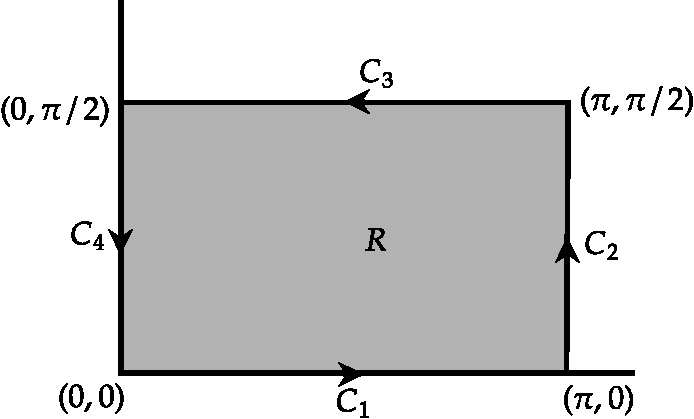
\includegraphics[height=3cm,width=5cm]{GT-Assignment-02}
		\end{figure}
		\begin{align*}
		\oint \vec{F} \cdot d \vec{r}&=\oint\left(x^{2}-y^{2}\right) d x+2 x y d y=\oint M d x+N d y\\
		\text{Here, }M&=x^{2}-y^{2}, \quad \frac{\partial M}{\partial y}=-2 y\\
		N&=2 x y, \quad \frac{\partial N}{\partial x}=2 y
		\intertext{Applying Green's theorem}
		 \oint M d x+N d y &=\iint\left(\frac{\partial N}{\partial x}-\frac{\partial M}{\partial y}\right) d x d y \\ &=4 \int_{0}^{b} \int_{0}^{a} y d x d y=4 a \int_{0}^{b} y d y \\ &=2 a b^{2} 
		\end{align*}
	\end{answer}
	
	
	
	
	
	
	
	
	
	
	
	
	
	
	
	
	
	
	
	
	
	
	
	
	
	
	
\end{enumerate}




%----------------------------------------------------------------------------------------
%	INDEX
%----------------------------------------------------------------------------------------

\cleardoublepage % Make sure the index starts on an odd (right side) page
\phantomsection
\setlength{\columnsep}{0.75cm} % Space between the 2 columns of the index
\addcontentsline{toc}{chapter}{\textcolor{ocre}{Index}} % Add an Index heading to the table of contents


%----------------------------------------------------------------------------------------

\end{document}
